\documentclass[11pt,a4paper,onecolumn,openright,oneside]{report}
\usepackage[square,sort&compress,comma,numbers]{natbib}
\usepackage[sectionbib]{chapterbib}
\usepackage[printonlyused,withpage]{acronym}
\usepackage[utf8]{inputenc}
\usepackage[T1]{fontenc}
\usepackage[top=2cm, bottom=2cm]{geometry}
\usepackage{float}%positionner les images
\usepackage{graphicx}%pour les images
\usepackage{soul}
\usepackage{enumitem}
\usepackage{makecell}
\usepackage{url}
\usepackage{tablefootnote}
\usepackage[colorlinks = true,
linkcolor = blue,
urlcolor  = blue,
citecolor = blue,
anchorcolor = blue
hyperfootnotes=false]{hyperref}

 \newcommand{\HRule}{\rule{\linewidth}{0.5mm}} %------- Faire les trai Dans La Page De Garde

%---- Begin Tableau Considérations pour les systèmes relationnels vs NoSQL
\usepackage{array,multirow,makecell} 
\newcolumntype{C}[1]{>{\centering\arraybackslash }b{#1}}
\newcolumntype{F}[1]{>{ \centering \vspace{1.mm} \arraybackslash}m{#1}<{ \vspace{1.mm}\arraybackslash }}
\newcolumntype{R}[1]{>{  \vspace{1.mm} \arraybackslash}m{#1}<{ \vspace{1.mm}\arraybackslash }}
\newcolumntype{G}[1]{>{ \centering \vspace{2.mm} \arraybackslash}m{#1}<{ \vspace{2.mm}\arraybackslash }}
%---- End Tableau Considérations pour les systèmes relationnels vs NoSQL

%------- Begin Ajouter les subsubsection à la table des matiere--------
\addtocounter{tocdepth}{3}
\setcounter{secnumdepth}{3}
%------- end Ajouter les subsubsection à la table des matiere--------

\usepackage{footnote} %------ Pur ressortir les note des élèment du tableau

\usepackage[french]{babel}

\usepackage{fancyhdr}

\usepackage{adjustbox}% pour orionté le tab 90°
\usepackage{amssymb}% pour chekmark dans le tableau
\makesavenoteenv{tabular}

\begin{document}
	\setcellgapes{3pt}
	
	\begin{titlepage}
		
		\begin{center}
			
			\textsc{\LARGE République Algérienne Démocratique et Populaire}\\
			\textsc{\LARGE Ministère de l’Enseignement Supérieur et de la Recherche Scientifique}\\
			\textsc{\LARGE Université Mouloud Mammeri de Tizi-Ouzou}\\
			
			\begin{figure}[H]
				\centering
				
\includegraphics[scale=1.5]{ummto.PNG}
			\end{figure}
			
			\textsc{\Large En vue de l’obtention du diplôme de Master Academique}\\
			\textsc{\Large Spécialité : Informatique}\\
			\textsc{\Large Options : Systèmes Informatiques et Ingénierie Des Systèmes d’information}\\[1cm]
			
			
			\textsc{\Large Thème}\\
			\HRule \\[0.5cm]
			% { \huge \bfseries Mise en place d'une solution web ERP \\
			% 	Cas: Œuvres Universitaires \\[0.4cm] }
            { \huge \bfseries Implémentation d'une solution web ERP \\
				Cas: Œuvres Universitaires \\[0.4cm] }
			
			\HRule \\[0.5cm]
			
			
			\emph{Présenté par :}\\
			
			Yanis \textsc{OUERDANE}\\
			Mohand \textsc{OURAD}\\[1.5cm]
			
			\emph{Devant le jury composé de :}\\
			
			\leftskip=4.5cm
			Président(e) : M$^{me}$ / M$^{elle}$ / M$^{r}$ JOHN Doe \\
			Examinateur(trice) : M$^{me}$ / M$^{elle}$ / M$^{r}$ DOE John\\
			Promoteur(trice) : M$^{me}$ \textsc{Goumeziane} Lynda \\ [1.5cm]
			
			
			\vfill
            {\large Année universitaire: 2020/2021}
			
		\end{center}
		
	\end{titlepage}

	\chapter*{\huge Remerciements}
	
	\begin{center}
		\it \Large
		D’abord, nous remercions le bon \textbf{DIEU} de nous avoir donné santé et courage pour réaliser ce travail.\\
		
		Nous tenons à exprimer notre profonde gratitude à notre encadreur \textbf{Mme GOUMEZIANE Lynda}, pour nous avoir encadré et guidé et surtout pour ses judicieux conseils qui ont contribué à alimenter notre réflexion.\\
		
		Nous remercions chaleureusement les membres de jury pour l’honneur qu’ils nous ont fait en acceptant de juger notre travail.\\
		
		Nos sincères sentiments vont à nos parents qui ont sacrifié jusqu’aujourd’hui et leurs encouragements tout le long de notre parcours.\\
		
		\leftskip=10cm 
		
		Yanis, Mohand.
		
		\leftskip=0cm
		
	\end{center}
	%------------------- End Remerciement ----------------------------
	
	\chapter*{\huge Dédicaces}
	
	\begin{center}
		\it \Large
		Je dédie ce modeste travail :
		A mes très chers parents que dieu les
		protègent, pour leur aide et leur soutien tout au long
		de mes études,\\
		
		A toute ma famille, à mes chers amis,\\
		
		Enfin à tous ceux qui ont contribué de près
		ou de loin pour la réalisation de ce travail.\\
		
		\leftskip=12cm
		
		Yanis.
		
		\leftskip=0cm
		
	\end{center}
    \chapter*{\huge Dédicaces}
	
	\begin{center}
		\it \Large
		Je dédie ce modeste travail :
		A mes très chers parents que dieu les
		protègent, pour leur aide et leur soutien tout au long
		de mes études,\\
		
		A toute ma famille, à mes chers amis,\\
		
		Enfin à tous ceux qui ont contribué de près
		ou de loin pour la réalisation de ce travail.\\
		
		\leftskip=12cm
		
		Mohand.
		
		\leftskip=0cm
		
	\end{center}
	
	\tableofcontents
	\listoffigures
	\addcontentsline{toc}{chapter}{Table des figures}
	\listoftables
	\addcontentsline{toc}{chapter}{Liste des tableaux}

	\section*{\Huge{Liste des Abréviations}}

\vspace{2em}

    \begin{acronym}
        \leftskip=1.5em

        \acro{ERP}{Enterprise Ressource Planning}
        \acro{PGI}{Progiciel de Gestion Intégré}
        \acro{MRP}{Manufacturing Resource Planning}
        
        \acro{D.O.U}{Diréction des Œuvres Universitaires}
        \acro{TIC}{Les Technologies de l’Information et de la Communication}
        
        \acro{PERN}{PostgreSQL, ExpressJS, React et NodeJS}
        \acro{MERN}{MongoDB, ExpressJS, React et NodeJS}
        \acro{CRUD}{Create, Read, Update, Delete}
    \end{acronym}

	\pagestyle{fancy}
	\fancyhead{}
	
	\renewcommand{\chaptermark}[1]{\markboth{\bsc{\chaptername~\thechapter{} :} #1}{}}
	
	% \rhead[\textsl{\leftmark}]{\textsl{\rightmark}}
	\lhead[\textsl{\rightmark}]{\textsl{\leftmark}}
	
	\renewcommand{\headrulewidth}{1.2pt}
	
	\newcommand\blfootnote[1]{
		\begingroup
		\renewcommand\thefootnote{}\footnote{#1}
		\addtocounter{footnote}{-1}
		\endgroup
	}

	\part*{Introduction Générale}
	\addcontentsline{toc}{part}{Introduction Générale}
		% \-\hspace{0.5cm} My internship within the department of roaming and international at Orange SA is a very important phase of my higher education. It is the transition point from university to start my professional career in the field of engineering. The field of mobile networks, roaming and the international environment gives me high motivation to learn as much as possible on my internship period in order to get my first position within this domain as an international roaming manager.\\

\section{Presentation and history of Orange}

\-\hspace{0.5cm} Orange is one of the world's leading telecommunications operators, with revenues of €42 billion and 147,000 employees on December 31, 2019, including 87,000 in France. The Group served 266 million customers as of December 31, 2019, including 207 million mobile customers and 21 million fixed broadband customers. The Group is present in 26 countries. Orange is also one of the world's leading providers of telecommunication services to multinational companies under the Orange Business Services brand \cite{pres-orange} (See annex 1 \cite{annex-one}).\\

\section{Roaming and International Department \acs{DRI} }
\-\hspace{0.5cm} The challenges of the Roaming and International department of Orange France are diverse, particularly because it is responsible for the Wholesale revenue generated by the entire Roaming activity. Among other things, it is responsible for defining the strategy and managing the entire Roaming activity for all Orange France entities (Business Markets, Consumer Markets, Finance, Legal, Technical), as well as expanding international coverage for Orange France customers for as many services as possible (\acs{2G}, \acs{SMS}, \acs{MMS}, \acs{CAMEL}, \acs{GPRS}, \acs{3G}, \acs{4G}, \acs{5G}, \acs{VOLTE}, etc.). The department has a staff of approximately 20 people and is divided into 3 departments (see annex 2) \\

	
	\part{Définitions Générales}
		% \chapter{Les Progiciels de Gestion Internes}

\section{Introduction}
Le but de ce chapitre est de présenter globalement le progiciel de gestion interne aussi appeler \acs{ERP}.\\

Dans un premier temps, nous définirons le concept d'\acs{ERP} et son évolution dans le temps.\\

Par la suite, nous aborderons les avantages liés a l'intégration d'un tel système dans les deux aspects administratif et opérationnel ainsi que ses inconvénients.\\

Nous finirons avec les multiples fonctionnalités de l'\acs{ERP}.\\

\section{Définition}
L'acronyme \acs{ERP} signifie Entreprise Resource Planning\cite{def-erp}, et sa similitude en français est Progiciel de Gestion Intégré abrévié \acs{PGI}.\\

Contrairement au \acs{MRP} (Manufacturing Resource Planning) qui se contente de la planification des besoins, l'\acs{ERP} est un logiciel qui permet la gestion de tous les sous-systèmes de l'entreprise et la coordination de ces sous-systèmes.\\

Pour y parvenir l’\acs{ERP} intègre toutes les fonctions utiles de l'entreprise sous forme de modules qui partagent une seule base de données, ce qui permet l'échange d'informations entre modules, dans ce cas, on parle de moteurs de workflow\footnote{"the sequence of steps involved in moving from the beginning to the end of a working process" - \href{https://www.merriam-webster.com/dictionary/workflow}{merriam-webster.com/dictionary - Definition of workflow}}.\\

\section{Historique}
Joseph Orlicky a été à l'origine de la création de l'\acs{ERP}.\cite{hist-erp} Il a créé l'acronyme de \acs{MRP} dans les années 1960, qui est l'ancêtre de la planification de la demande matérielle d'\acs{ERP}. \acs{MRP} répond principalement aux besoins de planification de l'entreprise.\\

Le concept d'\acs{ERP} tel que nous le connaissons est apparu pour la première fois dans les années 1990, mais avec l'avènement d'internet, il n'a commencé à se développer que dans les années 2000. L'utilisation de l'\acs{ERP} s'est généralisée et a évolué vers l'\acs{ERP} tel que nous le connaissons aujourd'hui.

\section{Avantages liés à l’intégration d’un \acs{ERP}}
Plusieurs études ont démontré les bénéfices de la mise en place d'un \acs{ERP}, dont l'une a été menée par Aberdeen Group,\cite{avantages} qui a quantifié et publié les résultats suivants :\\

\begin{itemize}
    \item Réduction des coûts d’opérations de 22\%
    \item Réduction des coûts d’administration de 20\%
    \item Réduction d’inventaires de 17\%
    \item Amélioration du temps de livraison de 19\%
    \item Amélioration du respect des délais et des budgets de 17\%\\
\end{itemize}

Même les entreprises en difficulté ont réalisé des avantages en intégrant l'\acs{ERP}, et le résultat est :\\

\begin{itemize}
    \item Réduction des coûts d’opérations de 7\%
    \item Réduction des coûts d’administration de 4\%
    \item Réduction d’inventaires de 9\%
    \item Amélioration du temps de livraison de 11\%
    \item Amélioration du respect des délais et des budgets de 6\%\\
\end{itemize}

Comme le souligne la recherche, les avantages en pourcentage ne semblent pas impressionnants, mais pour chaque million de dollars dépensé en coûts d'exploitation, des économies de 70 000 \$ sont réalisées.\\

En effet, on peut constater l'amélioration de la productivité et de la maturité des entreprises. Pour y parvenir, l'\acs{ERP} a été amélioré sous plusieurs aspects\cite{aspects} : \\

\subsection{Aspect administratif}
En consolidant tous les systèmes de l'entreprise en une seule application, l'installation de l'\acs{ERP} peut réduire les coûts d'exploitation et de maintenance, et parce que l'\acs{ERP} a une architecture modulaire, il fournit une infrastructure qui peut assurer la flexibilité à l'avenir lorsque des changements se produisent.\\

Une seule application, donc une seule base de données, cette seule base de données permet de gagner du temps. Réduire la quantité d'informations inutiles et évitez les saisies multiples. L'installation de l'\acs{ERP} résout le problème des informations incohérentes et fiabilise les données enregistrées.\\

De plus les activités manuelles de traitement, de comparaison et de recherche réalisée par les employés dans le cadre de l'interface des différents services sont évitées. Cela conduit à un gain de croissance, de temps et de productivité administrative.\\ 

\subsection{Aspect opérationnel}
L'utilisation de l'\acs{ERP} permet d'éliminer les risques opérationnels et les risques de pertes liés aux erreurs humaines ou aux défaillances du contrôle interne, et les fraudes qui peuvent être provoquées par les défaillances du système d'information existant. Les coûts supplémentaires inutiles dus aux dysfonctionnements sont réduits et une pertinence des informations partagées est gagnée.\\

L'\acs{ERP} permet également un suivi au niveau de l'achat jusqu'à la vente. En effet, dès la création de la commande, des données telles que la marge et le crédit sont générés automatiquement de manière dynamique pour réaliser l'intégration financière. Avec cette fonction, l'\acs{ERP} aide les managers dans le processus de planification et de prise de décision, et leur permet d'améliorer la gestion des ressources, ainsi améliorer la prise de décision opérationnelle.\\

De plus, les services de finances bénéficient de la centralisation. Cette centralisation permet de réunir les taches dans un seul endroit, ce qui a son tour permet l'amélioration de la productivité en réduisant le nombre d'employés nécessaires qui travaille sur la même tâche, cela permet d'augmenter les économies d’échelles notamment en matière de facturation.\\

\section{Inconvénients}
L'\acs{ERP} offre des avantages importants, mais une telle solution doit présenter certains inconvénients.\\

Les projets \acs{ERP} entraînent généralement des coûts lors de la configuration et de la maintenance. De plus, la complexité des programmes utilisés nécessite l'utilisation et la maintenance de serveurs puissants. Cela signifie que comme le montre l'étude CXP 2017\cite{cxp-2017}, les coûts sont souvent dépassés.\\

\begin{figure}[H]
    \centering
    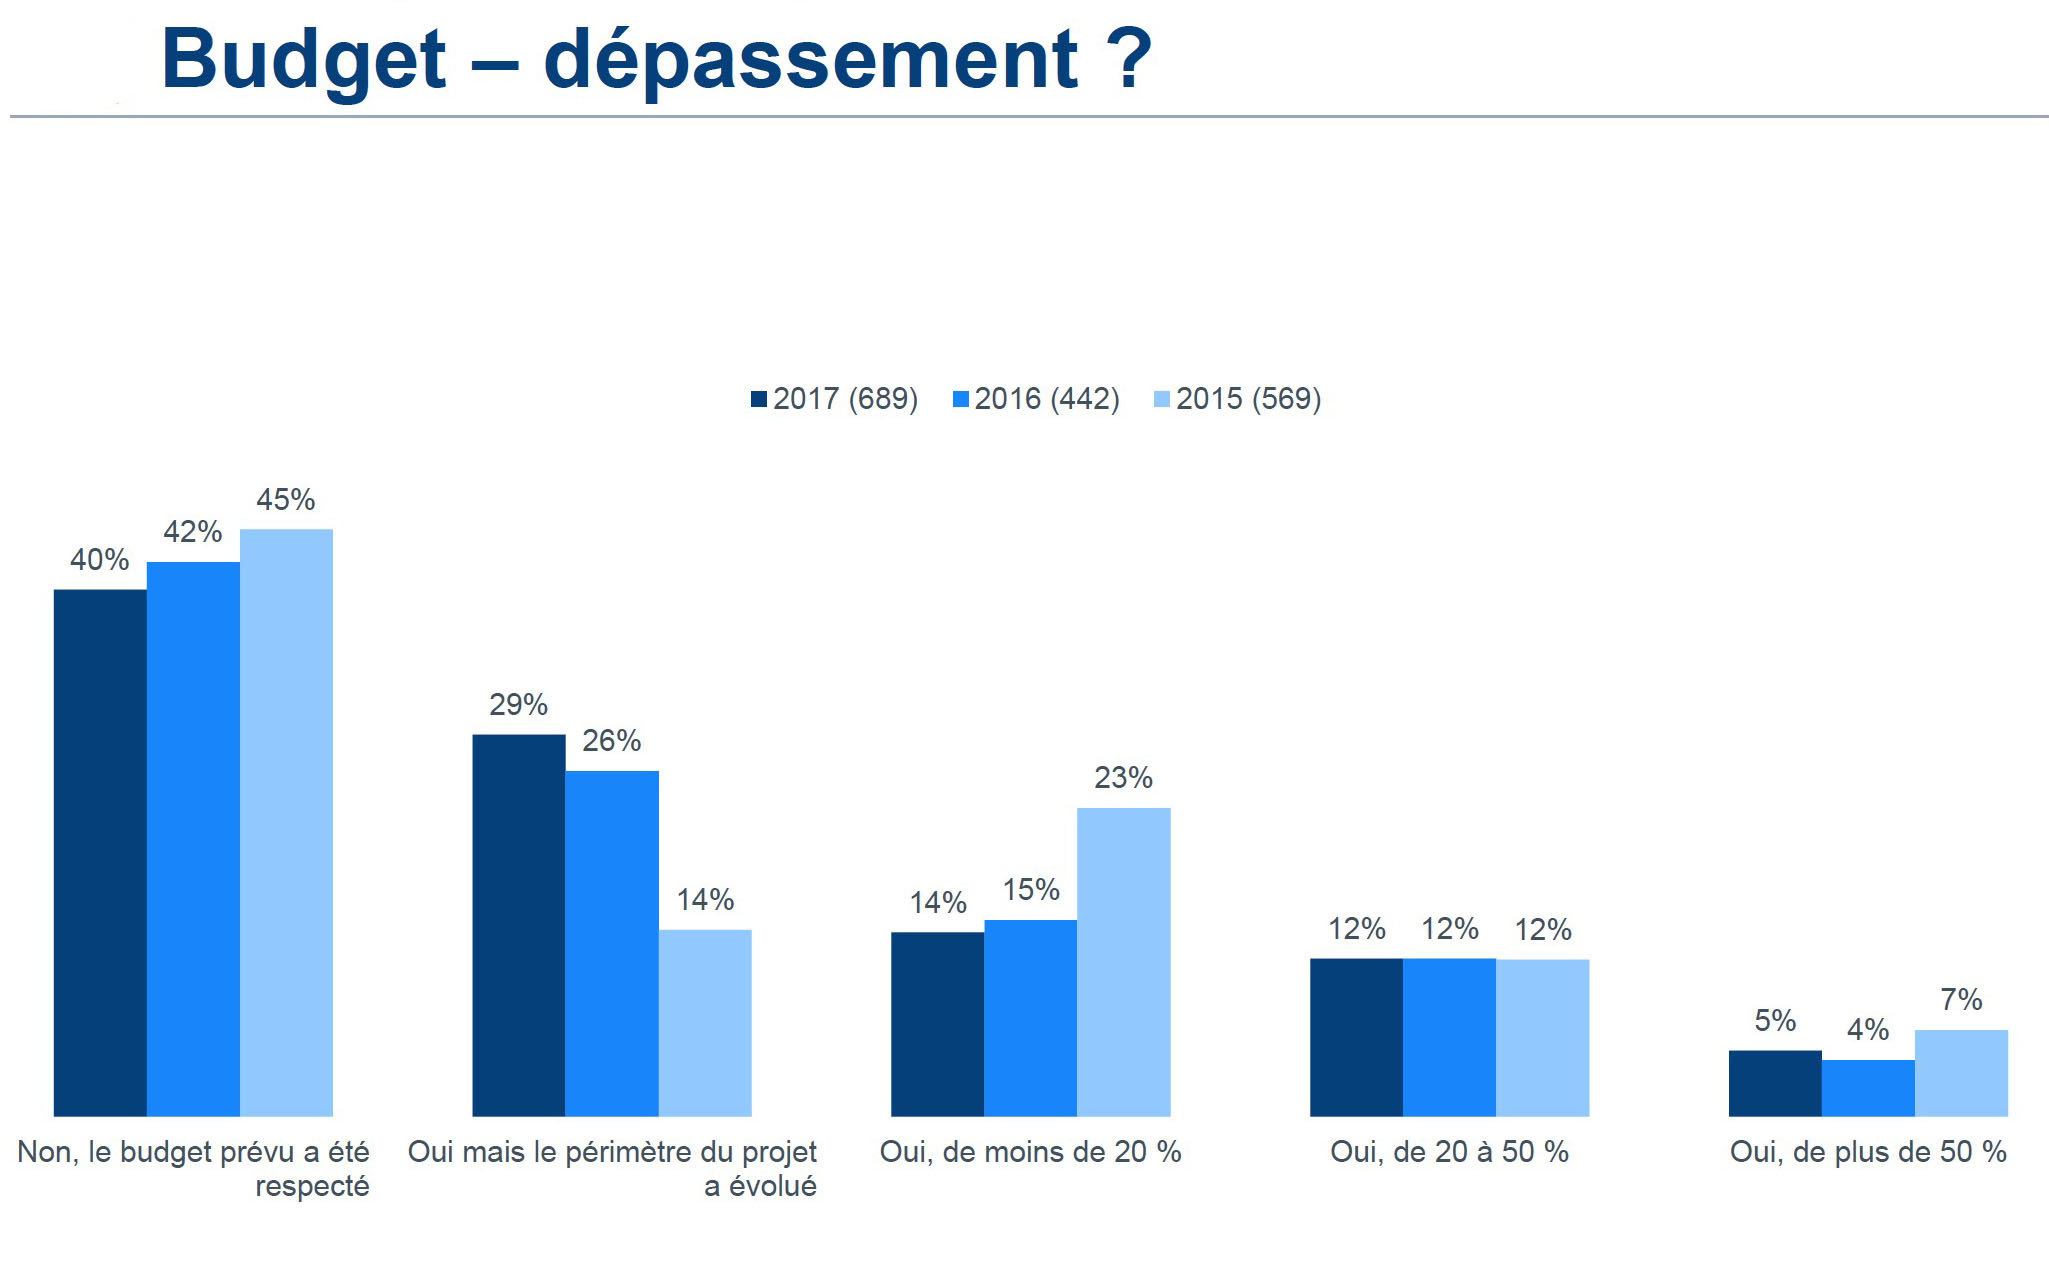
\includegraphics[scale=0.4]{ERP/graph-depassement-budget.jpg}
    \caption{Taux du dépassement de budget lors de l’implémentation d’un ERP}
\end{figure} 

On peut constater qu’en 2017 plus de 60\% des entreprises qui ont implémenté un \acs{ERP} ont dépassé le budget prévu, 58\% en 2016 et 55\% en 2015.\\

En plus du coût, comme le montre l'étude 2010 du rapport \acs{ERP} du cabinet de conseil Panorama Consulting\cite{panorama-consulting}, un projet d'une telle envergure peut nécessiter plus de temps et de ressources que prévu.\\

\begin{figure}[H]
    \centering
    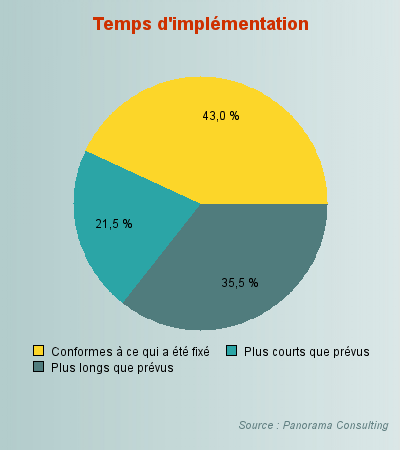
\includegraphics[scale=0.65]{ERP/graph-taux-implementation.png}
    \caption{Taux des dépassements des délais lors de l’implémentation d’un ERP}
\end{figure} 

Cette étude montre que plus de 35,5\% des entreprises ont mis en place un \acs{ERP} et constatent que le délai de mise en place a dépassé le délai autorisé. Il faut également noter que la durée moyenne de mise en place de l'\acs{ERP} est de 18 ou 4 mois, d'un éditeur à l'autre.\\

\section{Fonctionnalités}
Un \acs{ERP} est donc composé de modules\cite{modules}, ces modules son interconnecté et coexistent dans le système centralisé. Ce système centralisé est connecté à une seule base de données, ce qui donne l'avantage d'avoir tout un système et toutes les données requissent dans un seul endroit.\\

\begin{figure}[H]
    \centering
    
\includegraphics[scale=0.3]{ERP/erp-modules.png}
    \caption{Les modules d'un ERP}
\end{figure} 

Les besoins de chaque entreprise varient considérablement l'une de l'autre, mais l'\acs{ERP} donnent à celles-ci le pouvoir de choisir les modules dont elles ont vraiment besoin. Une entreprise orientée produite peut vouloir centraliser son inventaire et donc implémenter un module de gestion de stock, tandis qu'une entreprise orientée services pourront envisager l'implémentation d'un module de gestion de la relation clients.\\

Malgré leurs différences, ces deux types d'entreprise auront surement besoin de coordonner et gérer leurs employés ce qui les pousserait à envisager l'implementer d'un module de gestion des ressources humaine.\\

L'\acs{ERP} gère et organise automatiquement et dynamiquement les informations des différents services de l'entreprise, de l'approvisionnement des ressources aux ventes en passant par la production, ces fonctions\cite{funcs} sont nombreuses. Les modules les plus couramment utilisés sont :\\

\begin{itemize}
    \item Gestion de production
    \item Gestion de stock et d’inventaire
    \item Gestion des ressources humaines 
    \item Gestion de projet
    \item Gestion comptabilité
    \item Gestion commerciale
    \item Gestion d’achats
    \item CRM : Gestion des relations clients\\
\end{itemize}

Chaque module couvre ses propres fonctions, et le tableau suivant résume certains des modules et les fonctions qu'ils fournissent.

\begin{table}[H]
    \begin{center}
        
        \begin{tabular}{|F{4cm}|R{10cm}|}
            \hline
            \textbf{Modules}  & \makecell[c]{\textbf{Fonctionnalités}} \\
            \hline
            Achats
            &
            Gestion de toutes les transactions comptables, telle que les bons de commande pour l’approvisionnement. Etc.\\
            
            \hline
            Stock
            &
            Gestion des mouvements du stock, état du stock, entreposage.\\
            
            \hline
            Production
            &
            La gestion de la production, permet de réguler l’offre et les besoins en
            ressources par apport à la demande, impliquent la planification des ordres
            de fabrication et le contrôle de qualité.\\
            
            \hline
            Gestion de projet
            &
            Gestion de l’ensemble des projets de l’entreprise, de ces tâches et de ces plannings.\\
            
            \hline
            Ressources humaines
            &
            Gestion des ressources humaines et l’organisation de la rémunération des employés ainsi que des plannings de travail de ceux-ci.\\
            
            
            \hline
            Comptabilité
            &
            Gestion des obligations comptable auxquelles l’entreprise est soumise et suivie en temps réel de la santé financière de celle-ci, ainsi que de la gestion de facturation et des multidevises.\\
            
            \hline
            Commerciale
            &
            Gestion de l’aspect commerciale de l’entreprise, permet la gestion de l’ensemble des commandes clients et de leur facturation, permet aussi la réalisation de devis rapide et précise.\\
            
            \hline
            CRM
            &
            Gestion des relations clients, permet de réaliser de meilleurs suivis de
            l’environnement : clients, fournisseurs, prospects. etc.\\
            
            
            \hline
        \end{tabular}	
        \caption{Les Modules d'un \acs{ERP} et leurs fonctionnalités}
    \end{center}
\end{table}

\section{le marché des \acs{ERP}s}
Les \acs{ERP} en marché peuvent etre divisé en deux catégories: les \acs{ERP} open source et les \acs{ERP} propriétaires.

    \subsection{Les \acs{ERP} open source}
    Les \acs{ERP} open source sont ceux qui ont leurs code source est libre d'acces. Il est donc téléchargeable gratuitement et modifiable pour ajouter les fonctions nécessaires pour répondre aux besoins d'une entreprise ou la suppression des modules non nécessaire ou inutilisable déja existant.\\

    L'un des principaux leaders des \acs{ERP} open sources est nommée Odoo:

    \begin{figure}[H]
        \centering
        
\includegraphics[scale=0.1]{ERP/Odoo_logo.png}
        \caption{Logo Odoo}
    \end{figure} 

    Odoo\cite{odoo} est l'un des principaux logiciels \acs{ERP} open source, également connu sous le nom d'OpenERP\footnote{Open source \acs{ERP} - \acs{ERP} libre}. Il est composé de diverses applications et modules tels que le CRM, les ventes, la fabrication, la gestion de projet, les achats et la gestion des ressources humaines.\\

    Le développement et la mise en œuvre d'Odoo vous permet de choisir parmi des milliers de modules disponibles dans la boutique. Le logiciels \acs{ERP} Odoo fournit des services de bout en bout tels que la personnalisation, la mise en œuvre, l'intégration et l'assistance à la formation.\\

    \subsection{Les \acs{ERP} propriétaires}
    Les \acs{ERP} propriétaires sont les \acs{ERP} conçus par des entreprises qui ont une grande expertise dans la conception de logiciels et de systèmes informatiques. Comme tout \acs{ERP}, il contient différents modules qui répondent aux besoins des entreprises sauf que le système est fourni avec une licence payante, des limitations d'utilisation et des obligations et responsabilités dont le client doit suivre.\\
    
    L'avantage de ce type d'\acs{ERP} est de pouvoir profiter d'un savoir-faire reconnu, d'un accompagnement pendant toutes les étapes du projet d'ERP, d'un service personnalisé et dédié assurant la maintenance et le service après-vente.\\

    Parmi les leaders des \acs{ERP} propriétaires on peut citer SAP\cite{sap}, Microsoft Dynamics\cite{ms-dynamics} ou même Oracle \acs{ERP} Cloud\cite{oracle}.

    \begin{figure}[H]
        \centering
        
\includegraphics[scale=0.03]{ERP/SAP_logo.png}
        
\includegraphics[scale=0.3]{ERP/MS-Dynamics-Logopng.png}
        
\includegraphics[scale=0.2]{ERP/Oracle_Cloud_logo.jpg}
        \caption{Logo SAP, Microsoft Dynamics \& Oracle \acs{ERP} Cloud}
    \end{figure}

    Chacun de ces leaders propose sa propre solution que nous allons décrire dans le tableau suivant:

    \begin{table}[H]
        \begin{center}
            
            \begin{tabular}{|F{2.3cm}|R{3.5cm}|R{3.5cm}|R{3.5cm}|}
                \hline
                \textbf{ } & SAP & Microsoft & Oracle \\
                \hline
                Cible & \acs{PME}, \acs{ETI}, Grandes entreprises & \acs{PME}, \acs{ETI}, Grandes entreprises & \acs{PME}, \acs{ETI}, Grandes entreprises\\
                
                \hline
                Solution & SAP ERP, S/4 HANNA, S/4 Cloud, SAP Business One, SAP Business By Design & Oracle \acs{ERP} Cloud & Microsoft Dynamics 365\\
                
                \hline
                Modules
                &
                23 modules compris dans  3 catégories: Logistique, Comptabilité et RH
                &
                \begin{itemize}
                    \item Ventes
                    \item Marketing
                    \item Service
                    \item Finances
                    \item Opérations
                    \item Commerce
                    \item RH
                \end{itemize}
                &
                \begin{itemize}
                    \item Finances
                    \item Gestion de projets
                    \item Gestion de l'approvisionnement
                    \item Gestion des risques et conformité
                    \item Gestion des performances d'entreprise
                    \item Gestion de la chaîne d'approvisionnement et fabrication
                    \item Analytique 
                \end{itemize}
                \\

                \hline
                SGBD
                &
                SAP HANNA, Microsoft SQL Server, Oracle, My
                SQL.
                &
                Oracle Cloud
                &
                SQL Server
                \\
                
                \hline
            \end{tabular}	
            \caption{Description des solution \acs{ERP} propriétaires: SAP, Microsoft Dynamics et Oracle \acs{ERP} Cloud}
        \end{center}
    \end{table}    

\section{Conclusion}
Nous avons présenté l'\acs{ERP}, sa définition, son histoire au cours des années en plus des avantages, que ce sois dans l'aspect administratif ou opérationnel, et des inconvénients qu'il peut apporter.\\

Nous avons aussi montré qu'un \acs{ERP} peut être construit de plusieurs manières différentes et cela grâce à ses multiples fonctionnalités modulaires.\\

Dans le chapitre suivant, nous allons approfondir nos recherches et étudier le concept d'entreprise et la direction des œuvres universitaires.\\
		% \chapter{L'Entreprise et les Œuvres Universitaires}

\section{Introduction}
Dans ce chapitre nous commencerons par aborder le concept d'entreprise, une définition générale de celle-ci, son environnement économique et l'evolution des technologies de l'information et de la communication.\\

Nous passerons par la suite à la présentaion de l'organisme d'accueil qu'est la direction des œuvres universitaires (D.O.U) en général, son affiliation à l'office National des œuvres universitaires, ses missions et ses activités et son organisation administrative. 


Notre projet comprend la conception et la réalisation d'une application d'aide à la gestion des ressources de la direction des œuvres universitaires (D.O.U) en général. Celle-ci offre des services de transport, de restauration, de bourse, d'hébergement et d'activités scientifiques, culturelles et sportives. Ces mêmes services lui ont été délégués par l'Office National des œuvres universitaires en fonction de la wilaya où est siégée cette même \acs{D.O.U}.\\

À cet effet, il est nécessaire de définir un concept général d'une entreprise et de  présenter les services, en plus des missions, de la \acs{D.O.U} en tant qu'organisme d'accueil afin de comprendre leur principale activité.\\

\section{Concept d’Entreprise}
\subsection{Définition de l’entreprise \cite{def-entreprise}}
Une entreprise est un groupe d'unités légales qui se combinent pour créer une unité organisationnelle dont le but est de produire des biens ou des services. Il jouit d'une autonomie de décision dans l'affectation et l'utilisation de ses ressources disponibles.\\

Selon l'aspect économique, une entreprise est une unité qui produit des biens matériaux de consommation, de la matière première ou des services. Selon l'aspect sociologique cette unité est une structure avec des dirigeants, des salariés et des investisseurs.\\ 

Comme tout ensemble, chaque entité de cette unité à des intérêts qui peuvent différer des autres membres de l'entreprise. D'un côté, les investisseurs ses conscentre plus sur le rendement financier et des marges bénéficiaires sur le retour de leurs investissements, d'un autre côté, les dirigeants ont tendance à favoriser la performance, la croissance et la productivité de l'entreprise tout en s'assurant du bon contrôle et de la bonne gestion des salariés en pensant à minimisant les couts et les dépenses, tandis que les salariés, se focalisent sur leurs objectifs de réussite personnelle et professionnelle tout en s'assurant de bien accomplir leurs missions respectives.\\

Une entreprise publique, est une entreprise dont l'État dispose une part majoritaire du capital ou des voix attachées aux parts émises. L'État a donc le pouvoir d'exercer un contrôle direct ou indirect avec une influence dominante sur les décisions de cette dernière\cite{def-entreprise-pub}, par définition les \acs{D.O.U} prennent partie dans cette forme d'entreprise.\\

\subsection{Environnement Économique \cite{env-entreprise}}
L'environnement économoque d'une entreprise est un concept très large, il rassemble toutes les facteurs externes à celle-ci qui rentrent en rapport explicitement ou implicitement avec elle de manière a influencer les decisions de l'entreprise elle même. Les facteurs en question:\\

\begin{itemize}
    \item Le facteur démographique.
    \item le facteur économique.
    \item le facteur sociologique.
    \item le facteur technologique.
    \item le facteur politique et légale.
    \item le facteur écologique.
    \item le facteur de la concurrence et des produits de substitution.\\
\end{itemize}

Tous ces facteurs, participent donc, de près ou de loin, à la performance de l'entreprise dans son environnement\cite{perf-entreprise}. Les entreprises concurrentes voulant optimiser leurs processus et minimiser leurs dépenses se sont tourné vers les nouvelles technologies dont les systèmes d'informations, de gestion et de la communication.\\

\subsection{L’évolution des \acs{TIC} dans les entreprises}
Les technologies de l’information et de la communication ( \acs{TIC} ), sont un groupe de technologies qui permettent de transmettre, enregistrer, supprimer, modifier, crée et partager des informations sous forme numérique.\\ 

Les premières études sur les effets des \acs{TIC} sur la performance et la productivité avaient fait leur apparition en 1986 avec Robert Solow qui nota en premier le paradoxe qu’en pratique les \acs{TIC} n’avait pas d’effet positif sur la productivité contrairement à la théorie qui affirme le contraire.\\

Une autre analyse menée en 2002 sur l’utilisation des \acs{TIC} en entreprise, cette fois si à partir de données récentes indique une corrélation forte entre la performance, et la sophistication des équipements.\\

Ainsi avec l’évolution fulgurante des technologies grâce à la convergence de l’informatique, de la télécommunication et de l’internet. Les \acs{TIC} ont pris une nouvelle dimension et avec eux la montée en puissance des logiciels de gestion d’entreprises tels que les progiciels de gestion intégrée abrégée PGI ou en anglais ERP.\\

\section{La Direction des Œuvres Universitaires}
\subsection{Présentation de la \acs{D.O.U} \cite{dou}}
Les directions des œuvres Universitaires ont été créé conformément à l'arrêté interministériel du 22 décembre 2004 comportant la fixation de leurs sièges en plus de la liste constituant les résidences universitaires qui leur sont rattachées. Elles sont placées sous la tutelle de l'Office National des œuvres universitaires.\\

Elles sont chargées de veiller à la gestion des ressources financières et humaines, du bon déroulement et du contrôle des résidences universitaires dont elles sont responsables, de la gestion du transport entre les résidences et les différents établissements de l'enseignement supérieur et de la restauration, de la wilaya dont elles font partie.\\

\subsection{Missions et activités de la \acs{D.O.U} \cite{onou-arrete}}
Sa mission est de prendre en charge les différentes activités qui lui sont déléguées par l'Office National des œuvres universitaires qui est lui-même sous la tutelle du ministère de l'enseignement supérieur et de la recherche scientifique.\\

Principalement organiser et gérer les services d'hébergement, de restauration, de bourse, de transport et activités scientifique, culturelles et sportives, de manière à assurer la satisfaction des besoins de l’étudiants.\\

Plus précisément :

\begin{itemize}\renewcommand{\labelitemi}{$\bullet$}
    \item Veiller à la gestion des moyens matériels et financiers qui lui sont affectés.
    \item Prendre les mesures nécessaires au bon fonctionnement des structures placées sous son autorité.
    \item Veiller à la gestion de son personnel et du personnel des résidences universitaires sous son autorité.
    \item Veiller au bon contrôle rationnelle des moyens mis a la disposition des résidences universitaires sous son autorité.
    \item S'assurer, avec les structures et organismes concernés, du suivi des opérations d'investissement et d'équipement des résidences universitaires sous son autorité.
    \item Soumettre périodiquement des rapports sur le fonctionnement des résidences universitaires sous son autorité.
    \item Participer à la création et au bon suivi de l'application du règlement intérieur des résidences universitaires sous son autorité.
    \item Approuver et suivre le bon déroulement des programmes d'activités scientifiques, culturelles et de loisirs des résidences universitaires sous son autorité.
    \item Passez tout marché et contrat en relation avec la restauration et le transport assuré par les résidences universitaires sous son autorité.
    \item Exercer l'autorité hiérarchique sur son personnel.
    \item Nommer les personnels dont le mode de nomination n'est pas prévu.
    \item Ordonner les crédits qui lui sont délégués.
\end{itemize}

\subsection{L’organisation de la \acs{D.O.U} \cite{onou-arrete}}
La direction des œuvres universitaires est composée de 04 départements selon le diagramme suivant :

\begin{figure}[H]
    \centering
    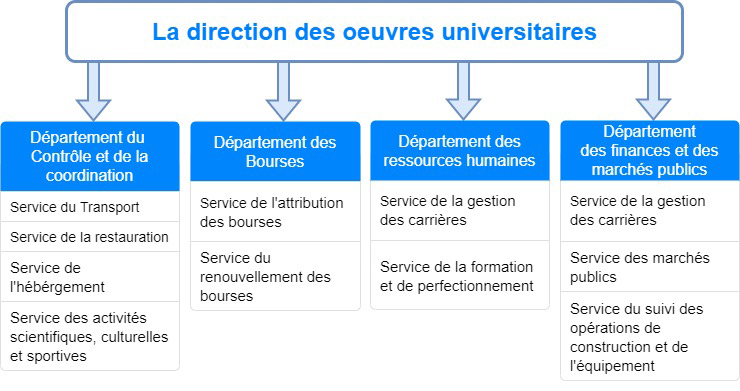
\includegraphics[scale=0.6]{DOU/direction-org.jpg}
    \caption{Organigramme de La Direction des Œuvres Universitaires}
\end{figure}

Chaque département regroupe plusieurs services qui sont chargé d'assurer différentes fonctions :

\subsubsection{Le département du controle et de la coordination}
\begin{itemize}
    \item Service du transport.
    \item Service de la restauration.
    \item Service de l'hébergement.
    \item Service des activités scientifiques, culturelles et sportives.\\
\end{itemize}

Ces différents services ont plusieurs taches différentes dont ils sont chargés d'exécuter et de veiller sur leur bonne exécution:

\paragraph{Hébérgement}
Le service d'hébergement comprend deux sections, la section de l'attribution de l'hébergement et la section de la gestion. À se fait, ce service a pour tâches :

\begin{itemize}
    \item Inscription des nouveaux bacheliers, et réinscription des anciens étudiants, ceci ce fait au niveau de chaque résidence.
    \item Contrôler les dossiers.
    \item Établir des statistiques sur l'état des résidences en rédigeant des listes globales de tous les étudiants et leurs répartitions par résidence et par bloc en tenant compte des nombres de places libres, les abandons, ... etc.
\end{itemize}

\paragraph{Transport}
\begin{itemize}
    \item Assurer le transport des étudiants des résidences universitaires vers les campus pédagogiques en tenant compte du trajet inverse.
\end{itemize}

\paragraph{Réstauration}
\begin{itemize}
    \item Assurer les repas au étudiants internes et externes.
\end{itemize}

\paragraph{Bourse}
\begin{itemize}
    \item Assurer le traitement et le suivi des dossiers des étudiants bénéficiaires de bourses.
    \item Assurer le renouvellement des bourses.
    \item Assurer le paiement régulier des bourses.
    \item Assurer le traitement et la prise en charge des bourses des étudiants étrangers.\\
\end{itemize}

Ce département est chargé de :
\begin{itemize}\renewcommand{\labelitemi}{$\bullet$}
    \item Mettre en œuvre les plans de transport universitaire des résidences universitaires rattachées à la \acs{D.O.U} et superviser le processus jusqu'à son aboutissement.
    \item Superviser, surveiller et orchestrer les actes d'œuvre universitaires assurées par les résidences universitaires associées à la \acs{D.O.U}.
    \item Présenter des méthodes rationnelles d'utilisation de tous les moyens dédiés aux activités des œuvres universitaires.
    \item Contrôler, et Assurer la bonne application des programmes d'activités scientifiques, et sportives approuvées par le directeur de la direction.\\
\end{itemize}

\subsubsection{Le département des ressources humaines}
\begin{itemize}
    \item Service de la gestion des carrières.
    \item Service de la formation et de perfectionnement.\\
\end{itemize}

Ce département est chargé de :
\begin{itemize}\renewcommand{\labelitemi}{$\bullet$}
    \item La gestion de la carrière du personnel de la \acs{D.O.U}.
    \item L'implémentation des plans de formation et perfectionnement du personnel de la \acs{D.O.U}.
\end{itemize}

\subsubsection{Le département des bourses}
\begin{itemize}
    \item Service de l'attribution des bourses.
    \item Service du renouvellement des bourses.\\
\end{itemize}

Ce département est chargé de :
\begin{itemize}\renewcommand{\labelitemi}{$\bullet$}
    \item Suivre et garantir le traitement des dossiers des étudiants bénéficiaires de bourses.
    \item Garantir le paiement régulier des bourses.
    \item Prendre en charge et garantir le traitement des bourses des étudiants étrangers.
\end{itemize}

\subsubsection{Le département des finances et des marchés publics}
\begin{itemize}
    \item Service du budget et de la comptabilité.
    \item Service des marchés publics.
    \item Service du suivi des opérations de construction et de l'équipement.\\
\end{itemize}

Ce département est chargé de :
\begin{itemize}\renewcommand{\labelitemi}{$\bullet$}
    \item Gérer les moyens matériels et financiers qui ont été mis à la disponibilité de la \acs{D.O.U}.
    \item Garantir de service de traitements des personnels de la \acs{D.O.U}.
    \item Garantir le contrôle des divers étapes de passation des marchés publics et d'en surveiller l'exécution par les résidences universitaires.
    \item Garantir, en conjonction avec les services concernés, la surveillance des actes de construction et d'équipement des résidences universitaires.\\
\end{itemize}

\section{La Problématique}
Parmi les problèmes qui existent après l’analyse de ce système, on peut citer :
\begin{itemize}
    \item Le transfert de données entre la \acs{D.O.U} et les différentes résidences se fait manuellement.
    \item La répartition des étudiants d’une manière arbitraire, ce qui engendre l’augmentation de l’enveloppe budgétaire alloue au transport.
    \item La perte de temps.
    \item La non disponibilité des informations au bon moment.
    \item La \acs{D.O.U} dispose d'un réseau informatique à haut débit mais très mal exploité. En fait, il n'existe aucune application ou logiciel fonctionnant sous réseau.
    \item La grande difficulté d'accéder aux informations en tant qu'étudiants. Les seules moyens qui existent actuellement sont des pages facebook, des photos de fiches mal prise et des sites internet existant mais qui ne marches pas et/ou ne contient pas les informations pertinente dont l'étudiant a besoin.
    \item La non existence des informations concernant les repas des services de restauration.
    \item L'inconsistance et l'incohérence des informations.\\
\end{itemize}

\section{Présentation de la solution}
Afin de remédier aux problèmes cités ci-dessus. Nous avons proposé de concevoir une application de gestion de ressources en se basant sur les Progiciels de Gestion Intégré \acs{ERP}, ceci pour permettre de :\\

\begin{itemize}
    \item Informatiser l'ajout, la validation et le rejet des dossiers.
    \item Informatiser la liste des résidences et des campus universitaires.
    \item Automatiser la gestion des trajets du service des transports.
    \item Rendre public les informations sur les services de restauration et de transport notamment les menus des restaurants universitaires et les trajets des bus universitaires. 
    \item Informatiser l'affectation des étudiants aux résidences.
    \item Informatiser la gestion de la restauration, notamment les ingrédients, les plats, les menus et le calendrier des menus.
    \item Avoir une plateforme centraliser pour la gestion de tous les services du département du contrôle et de la coordination, voire plus.
    \item Avoir un rapport mensuel des menus, des ingrédients et des plats du service de la restauration.
    \item Avoir un rapport mensuel des trajets et des bus du service des transports.
    \item Normaliser et regrouper les informations concernant les \acs{D.O.U}.\\
\end{itemize}

\section{Conclusion}
Dans ce chapitre nous avons abordé les concepts de base d'entreprise, et l'organisme d'accueil qu'est la direction des œuvres universitaires.\\

Nous avons par la suite présenté les missions et les activités de l'organisme d'accueil tout en détaillant l'organisation départementale de ce dernier, en prenant compte des services et des tâches qui leur sont rattachées.\\

En dernier, nous avons retenu plusieurs problèmes qui sont liés particulièrement à une mauvaise gestion des ressources en plus d’une retenue de l’information et le traitement manuel de l'information, tout en citant une présentation simple d'une solution a ces derniers.\\

Le chapitre suivant sera consacrée à l'analyse plus détailler du système et des ses besoins, et une conception des solutions de notre application.

\newpage

\leftskip=0cm
\renewcommand{\bibname}{Référence bibliographique et webographique du chapitre 2}
\bibliographystyle{ieeetr}	
\bibliography{DOU/dou}

	\part{Analyse, Conception \& Réalisation}
		\chapter{Analyse \& Conception}

\section{Introduction}
Le but de ce chapitre est d'aborder les concepts essentiels a la réalisation du projet.\\

En première partie, nous ferons un rappel sur les généralités d'UML, sa définition et ses diagrammes.\\

Par la suite, nous passerons à l'analyse des principaux utilisateurs du système et les besoins de ces derniers.\\

Nous terminerons par une conception des diagrammes de classes et des diagrammes de séquences ainsi qu'une présentation de la structure de la base de données.\\

\section{Présentation d'\acs{UML}}
\acs{UML}\cite{uml-diag} est un acronym qui signifie Unified Modeling Langage ou Langage de Modélisation Unifié en français, est apparu pour la première fois dans les années 1990. En simple, \acs{UML} est une approche moderne et méthodique de la modélisation et de la documentation des applications. C'est l'une des techniques de modélisation des processus d'entreprise les plus populaires.\\

Son approche est basée sur des représentations schématiques des composants d'un logiciel. Cette représentations visuelles nous donnent la possibilité de mieux mesurer les éventuelles erreurs ou défauts des logiciels.\\

\subsection{Les diagrammes \acs{UML}}
La représentation graphique des composants d'un logiciel\cite{uml-diag} et faites à l'aide de diagrammes. Ces diagrammes sont simples, stricte et contiennent des règles d'utilisations et de syntaxes bien fix.\\

UML nous permet d'établire une représentation du logiciel sous plusieurs angles ou vues:

\begin{itemize}
    \item \textbf{Vue des cas d’utilisation} : vue des acteurs (besoins attendus)
    \item \textbf{Vue logique} : vue de l'intérieur (satisfaction des besoins)
    \item \textbf{Vue d’implantation} : dépendances entre les modules
    \item \textbf{Vue des processus} : dynamique du système
    \item \textbf{Vue de déploiement} : organisation environnementale du logiciel
\end{itemize}

UML est composé de plusieurs diagrammes chacun d'eux sert à des objectifs différent qu'il soit avant ou après la mise en oeuvre.

\section{Analyse}
La phase d’analyse débute par l'identification des acteurs ainsi que leurs différentes tâches dans le système, ensuite, la spécification des besoins fonctionnels et non fonctionelles du système. Ceci nous mène vers une schématisation par un diagramme des cas d’utilisation traduisant la dynamique système qui sera utilisé dans la phase de conception.


\subsection{Spécification des besoins}
\subsubsection{Besoins fonctionnels}
C’est une description des caractéristiques du système et de ses fonctionnalités. En partant de ce principe notre application doit permettre :\\

    \textbf{Visiteurs\\}
        \textbf{Consultation de la page d’accueil}
        \begin{itemize}
            \item Consulter le service d'hébergements
            \item Télécharger le document d'aide à la constitution du dossier d'hébergement
            \item Consulter le service de restauration
            \item Consulter le service des transports
            \item Consulter le service des bourses
            \item Télécharger le document d'aide à la constitution du dossier de bourse
            \item Télécharger le document d'aide au renouvellement du dossier de bourse
            \item Télécharger le document d'aide au transfert du dossier de bourse\\
        \end{itemize}

        \textbf{Consultation du calendrier des menus de chaque restaurant d'un mois défini}
        \begin{itemize}
            \item Changer le mois du calendrier des menus
            \item Changer l'affichage des menus par mois, semaine, jour de travail, jour et par agenda
            \item Voir plus d'informations sur un seul menu\\
        \end{itemize} 
        
        \textbf{Consultation du calendrier de tous les trajets de chaque Campus/Résidence d'un mois défini}
        \begin{itemize}
            \item Changer le mois du calendrier des trajets
            \item Changer l’affichage des trajets par mois, semaine, jour de travail, jour et par agenda
            \item Voir plus de détails sur un seul trajet \\
        \end{itemize}

\textbf{Staff\\}
En plus des fonctionnalités du visiteur le staff peut aussi:\\

    \textbf{Hébergement}
    \begin{itemize}
        \item Consulter la liste des dossiers d'hébergement
        \item Sélectionner un ou plusieurs dossiers d'hébergement
        \item Ajouter un dossier d'hébergement
        \item Supprimer un ou plusieurs dossier(s) d'hébergement
        \item Voir plus d'informations sur un dossier d'hébergement
        \item Valider un dossier d'hébergement
        \item Refuser un dossier d'hébergement \\
    \end{itemize}

    \textbf{Bourse}
    \begin{itemize}
        \item Consulter la liste des dossiers de bourse
        \item Sélectionner un ou plusieurs dossiers de bourse
        \item Ajouter un dossier de bourse
        \item Supprimer un ou plusieurs dossier(s) de bourse
        \item Voir plus d'informations sur un dossier de bourse
        \item Valider un dossier de bourse
        \item Refuser un dossier de bourse
        \item Changer l'ordre d'affichage par attributs \\
    \end{itemize}

    \textbf{Campus \& Résidences}
    \begin{itemize}
        \item Consulter la liste des Campus \& Résidences
        \item Ajouter un campus ou une résidence
        \item Supprimer un campus ou une résidence
        \item Voir plus d'informations sur un campus ou une résidence
        \item Modifier les informations d'un campus ou une résidence
        \item Rechercher un campus ou une résidence
        \item Filtrer par campus seulement résidences seulement ou par campus \& résidences \\
    \end{itemize}

    \textbf{Transport - Calendrier}
    \begin{itemize}
        \item Voir les trajets détaillé de tout le mois
        \item Ajouter un trajet
        \item Modifier un trajet
        \item Supprimer un trajet \\
    \end{itemize}

    \textbf{Transport - Bus}
    \begin{itemize}
        \item Consulter la liste des bus
        \item Sélectionner un ou plusieurs bus
        \item Ajouter un bus
        \item Supprimer un ou plusieurs bus
        \item Voir plus d'informations sur un bus
        \item Modifier les informations d'un bus
        \item Filtrer par attributs \\
    \end{itemize}

    \textbf{Restauration - Calendrier}
    \begin{itemize}
        \item Voir les menus détaillé de tout le mois par semaine
        \item Ajouter un menu
        \item Modifier un menu
        \item Supprimer un menu \\
    \end{itemize}

    \textbf{Restauration - Restaurants}
    \begin{itemize}
        \item Consulter la liste des restaurants
        \item Ajouter un restaurant
        \item Supprimer un restaurant
        \item Voir plus d'informations sur un restaurant
        \item Modifier les informations d'un restaurant
        \item Rechercher un restaurant
        \item Filtrer par les restaurants par établissements ( appartiennent à un campus ou une résidence )\\
    \end{itemize}

    \textbf{Restauration - Plats \& Desserts}
    \begin{itemize}
        \item Consulter la liste des plats \& desserts
        \item Ajouter un plat/dessert
        \item Supprimer un plat/dessert
        \item Voir plus d'informations sur un plat/dessert
        \item Modifier les informations d'un plat/dessert
        \item Rechercher un plat/dessert
        \item Filtrer par plats seulement desserts seulement ou par plats \& desserts\\
    \end{itemize}

    \textbf{Restauration - Ingrédients}
    \begin{itemize}
        \item Consulter la liste des ingrédients
        \item Sélectionner un ou plusieurs ingrédient(s)
        \item Ajouter un ingrédient
        \item Supprimer un ou plusieurs ingrédient(s)
        \item Voir plus d'informations sur un ingrédient
        \item Modifier les informations d'un ingrédient
        \item Filtrer par attribut\\
    \end{itemize}

    \textbf{Administrateur\\}
    En plus des fonctionnalités de l'utilisateur l'administrateur peut aussi: \\
    \textbf{Utilisateurs}
    \begin{itemize}
        \item Consulter la liste des utilisateurs
        \item Sélectionner un ou plusieurs utilisateur(s)
        \item Ajouter un utilisateur
        \item Supprimer un ou plusieurs utilisateur(s)
        \item Voir plus d'informations sur un utilisateur
        \item Modifier les informations d'un utilisateur
        \item Filtrer par attributs\\
    \end{itemize}

\subsubsection{Besoins non fonctionnels}
Ça représente des exigences qui ne concernent pas le comportement du système. Elles identifient les contraintes internes et externes du système. Dans notre cas l’application devra respecter les exigences suivantes :\\

\noindent \textbf{Performance:} temps de réponse petit.\\
\textbf{Maintenabilité:} apporter des corrections facilement.\\
\textbf{Fiabilité:} précise et correcte.\\
\textbf{Intégrabilité:} intégrer de nouvelles fonctionnalités facilement.\\
\textbf{Portabilité:} elle peut fonctionner sur plusieurs plateformes.\\
\textbf{Disponibilité:} réaliser une fonction requise à tout moment.\\
\textbf{Sécurité:} personnaliser les accès selon l’utilisateur.\\

\subsection{Identification des acteurs}
Un acteur est une entité externe qui a la possibilité d'interagir et d'utiliser les multiples fonctionnalités du système.

\subsubsection{Les acteurs qui interviennent dans notre système}
\begin{itemize}
    \item \textbf{L’administrateur :} C’est le cerveau de l’application, il gère toutes les fonctions de l’application ainsi que les utilisateurs et leurs rôles dans le site.
    \item \textbf{L'utilisateur/staff :} Un staff est un gérant, il a un accès global aux fonctions de l'application hormis les fonctions liées aux utilisateurs.
    \item \textbf{Le visiteur :} il peut uniquement consulter le contenu du site.
\end{itemize}

\subsubsection{Diagramme de contexte}
Le diagramme de contexte, comme son nom l'indique, nous permet de bien comprendre de contexte de notre application et des acteurs qui y participent. Il nous permet d'avoir une vue globale sur les utilisateurs du système:

\begin{figure}[H]
    \centering
    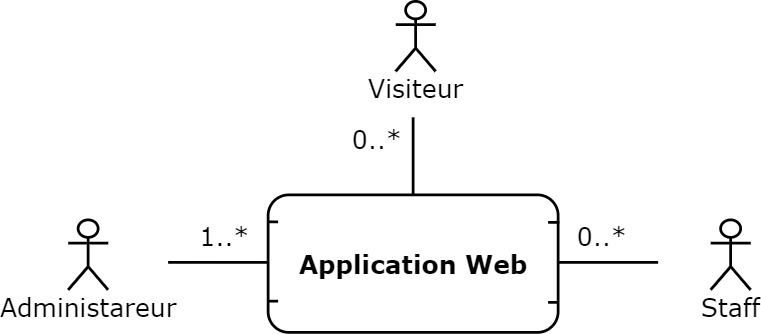
\includegraphics[scale=0.5]{ACR/Diagrammes/contexte.jpg}
    \caption{Diagramme de contexte}
\end{figure}

\subsection{Spécification des tâches}
Dans ce point, nous allons spécifier les tâches de chaque acteur. Le tableau suivant résume ces tâches :

\begin{longtable}{|Z{3cm}|L{10cm}|}
    \caption{Spécification des tâches liées à chaque acteur}\\
    \hline
    \textbf{Acteur} & \textbf{Tâches} \\
    \hline
    \endfirsthead
    \multicolumn{2}{c}%
    {\tablename\ \thetable\ -- \textit{(Suite) Spécification des tâches liées à chaque acteur}} \\
    \hline
    \textbf{Acteur} & \textbf{Tâches} \\
    \hline
    \endhead
    \hline \multicolumn{2}{r}{\textit{(À suivre) Spécification des tâches liées à chaque acteur}} \\
    \endfoot
    \hline
    \endlastfoot
    Visiteurs &
        \textbf{T01 - Consultation de la page d’accueil}
        \begin{itemize}
            \item Consulter le service d'hébergements
            \item Télécharger le document d'aide à la constitution du dossier d'hébergement
            \item Consulter le service de restauration
            \item Consulter le service des transports
            \item Consulter le service des bourses
            \item Télécharger le document d'aide à la constitution du dossier de bourse
            \item Télécharger le document d'aide au renouvellement du dossier de bourse
            \item Télécharger le document d'aide au transfert du dossier de bourse
        \end{itemize} \\
        &
        \textbf{T02 - Consultation du calendrier des menus de chaque restaurant d'un mois défini}
        \begin{itemize}
            \item Changer le mois du calendrier des menus
            \item Changer l'affichage des menus par mois, semaine, jour de travail, jour et par agenda
            \item Voir plus d'informations sur un seul menu
        \end{itemize} \\
        &
        \textbf{T03 - Consultation du calendrier de tous les trajets de chaque Campus/Résidence d'un mois défini}
        \begin{itemize}
            \item Changer le mois du calendrier des trajets
            \item Changer l’affichage des trajets par mois, semaine, jour de travail, jour et par agenda
            \item Voir plus de détails sur un seul trajet
        \end{itemize}
     \\
     \hline
    & \\ &
    En plus des fonctionnalités du visiteur le staff peut aussi:\\
    Staff &
    \textbf{T01 - Hébergement}
    \begin{itemize}
        \item Consulter la liste des dossiers d'hébergement
        \item Sélectionner un ou plusieurs dossiers d'hébergement
        \item Ajouter un dossier d'hébergement
        \item Supprimer un ou plusieurs dossier(s) d'hébergement
    \end{itemize}\\
    &
    \begin{itemize}
        \item Voir plus d'informations sur un dossier d'hébergement
        \item Valider un dossier d'hébergement
        \item Refuser un dossier d'hébergement
    \end{itemize}\\
    &
    \textbf{T02 - Bourse}
    \begin{itemize}
        \item Consulter la liste des dossiers de bourse
        \item Sélectionner un ou plusieurs dossiers de bourse
        \item Ajouter un dossier de bourse
        \item Supprimer un ou plusieurs dossier(s) de bourse
        \item Voir plus d'informations sur un dossier de bourse
        \item Valider un dossier de bourse
        \item Refuser un dossier de bourse
        \item Changer l'ordre d'affichage par attributs
    \end{itemize}\\ &
    \textbf{T03 - Campus \& Résidences}
    \begin{itemize}
        \item Consulter la liste des Campus \& Résidences
        \item Ajouter un campus ou une résidence
        \item Supprimer un campus ou une résidence
        \item Voir plus d'informations sur un campus ou une résidence
        \item Modifier les informations d'un campus ou une résidence
        \item Rechercher un campus ou une résidence
        \item Filtrer par campus seulement résidences seulement ou par campus \& résidences
    \end{itemize}\\
    &
    \textbf{T04 - Transport - Calendrier}
    \begin{itemize}
        \item Voir les trajets détaillé de tout le mois
        \item Ajouter un trajet
        \item Modifier un trajet
        \item Supprimer un trajet
    \end{itemize}\\
    &
    \textbf{T05 - Transport - Bus}
    \begin{itemize}
        \item Consulter la liste des bus
        \item Sélectionner un ou plusieurs bus
        \item Ajouter un bus
        \item Supprimer un ou plusieurs bus
        \item Voir plus d'informations sur un bus
        \item Modifier les informations d'un bus
        \item Filtrer par attributs
    \end{itemize}\\
    &
    \textbf{T06 - Restauration - Calendrier}
    \begin{itemize}
        \item Voir les menus détaillé de tout le mois par semaine
        \item Ajouter un menu
        \item Modifier un menu
        \item Supprimer un menu
    \end{itemize}\\ &
    \textbf{T07 - Restauration - Restaurants}
    \begin{itemize}
        \item Consulter la liste des restaurants
        \item Ajouter un restaurant
        \item Supprimer un restaurant
        \item Voir plus d'informations sur un restaurant
        \item Modifier les informations d'un restaurant
        \item Rechercher un restaurant
        \item Filtrer par les restaurants par établissements ( appartiennent à un campus ou une résidence )
    \end{itemize}\\
    &
    \textbf{T08 - Restauration - Plats \& Desserts}
    \begin{itemize}
        \item Consulter la liste des plats \& desserts
        \item Ajouter un plat/dessert
        \item Supprimer un plat/dessert
        \item Voir plus d'informations sur un plat/dessert
        \item Modifier les informations d'un plat/dessert
        \item Rechercher un plat/dessert
        \item Filtrer par plats seulement desserts seulement ou par plats \& desserts
    \end{itemize}\\
    &
    \textbf{T09 - Restauration - Ingrédients}
    \begin{itemize}
        \item Consulter la liste des ingrédients
        \item Sélectionner un ou plusieurs ingrédient(s)
        \item Ajouter un ingrédient
        \item Supprimer un ou plusieurs ingrédient(s)
        \item Voir plus d'informations sur un ingrédient
        \item Modifier les informations d'un ingrédient
        \item Filtrer par attribut
    \end{itemize} \\
    \hline & \\ Administrateur & 
    En plus des fonctionnalités de l'utilisateur l'administrateur peut aussi:\\
    & \\ &
    \textbf{T01 - Utilisateurs}
    \begin{itemize}
        \item Consulter la liste des utilisateurs
        \item Sélectionner un ou plusieurs utilisateur(s)
        \item Ajouter un utilisateur
        \item Supprimer un ou plusieurs utilisateur(s)
        \item Voir plus d'informations sur un utilisateur
        \item Modifier les informations d'un utilisateur
        \item Filtrer par attributs
    \end{itemize}
\end{longtable}

\subsection{Représentation des diagrammes des cas d'utilisation}
Il répond à la question "Comment les participants au système interagissent-ils avec lui ?". En d'autres termes, le diagramme de cas d'utilisation permet de définir la relation entre le système et les participants.

\subsubsection{Diagramme des cas d’utilisation global}
\paragraph*{Remarque} Les cas d'utilisation de l'acteur "staff" sont nombreux, pour ceux et pour ne pas encombré le diagramme des cas d'utilisation global, nous avons omis les détails de cette acteur puis détaillées, plus bas, les cas d'utilisation spécifiques. \textbf{Les cas dont les détailes son omis sont marqué par un asterics "*"}\\

\begin{figure}[H]
    \centering
    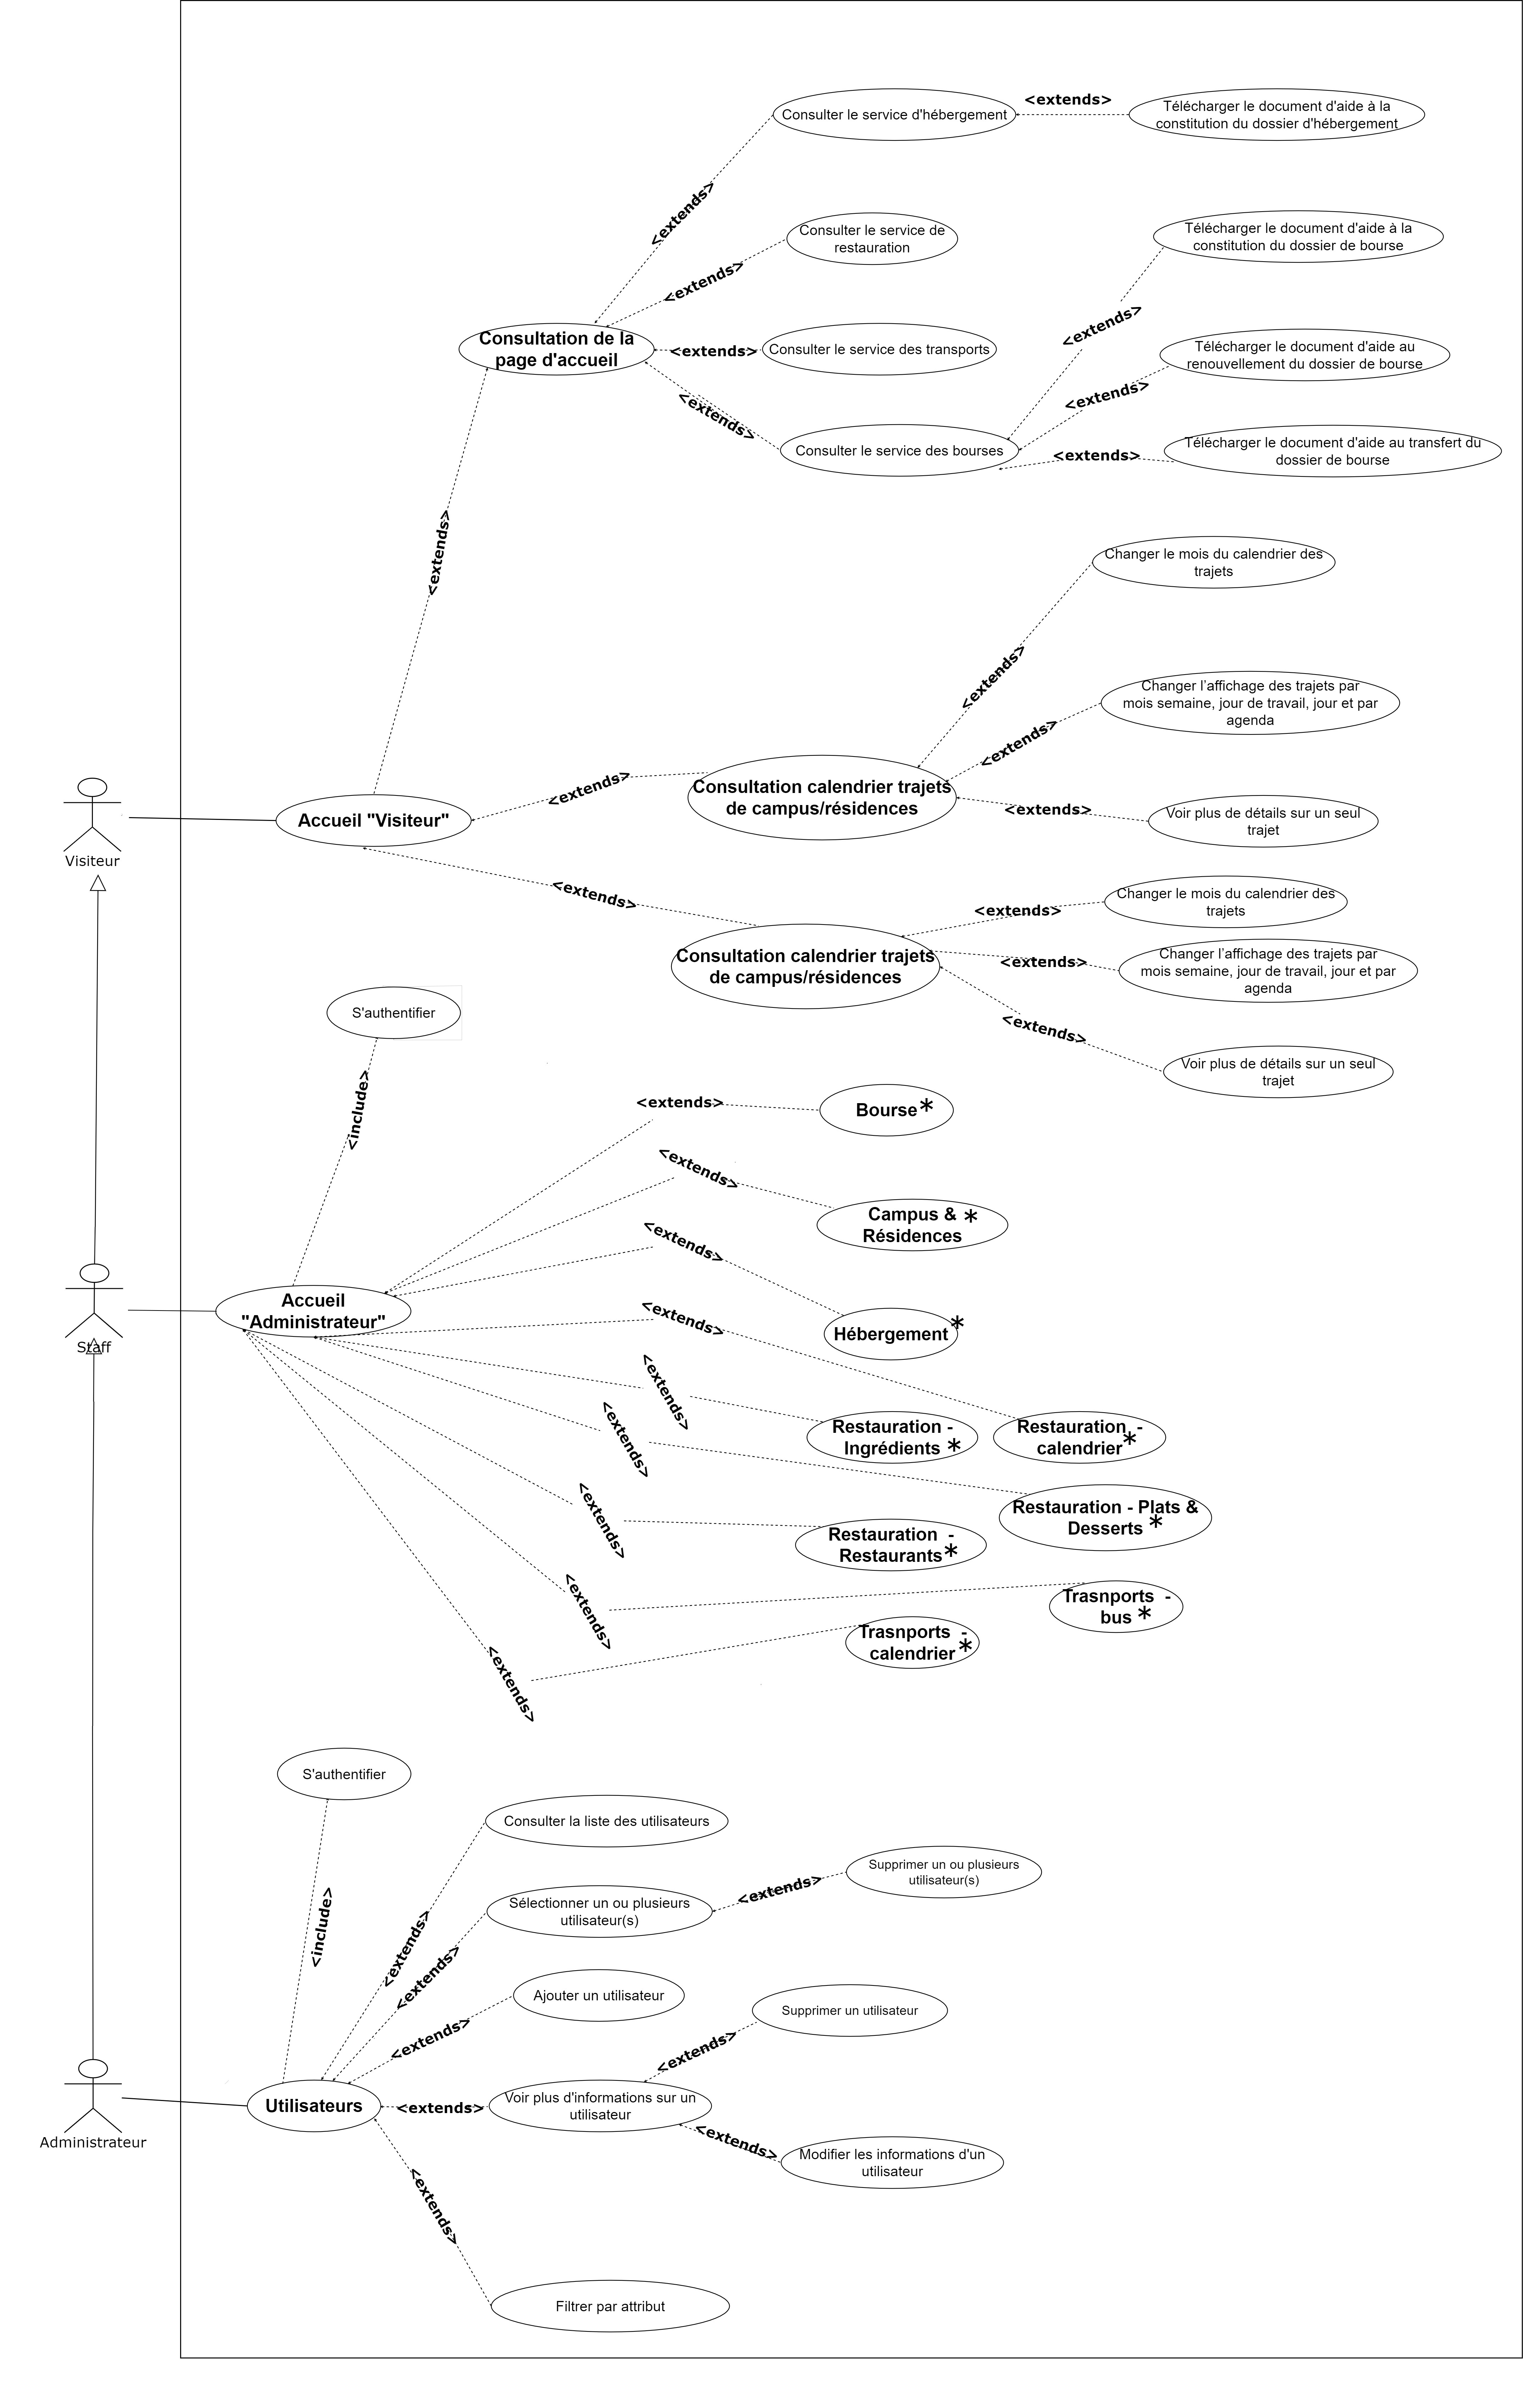
\includegraphics[scale=0.1]{ACR/Diagrammes/Global (1).jpg}
    \caption{Cas d'utilisation global}
\end{figure}

\subsubsection{Diagrammes des cas d’utilisation détaillés}

\subsubsection*{Cas d'utilisation 'Bourses'}
\begin{figure}[H]
    \centering
    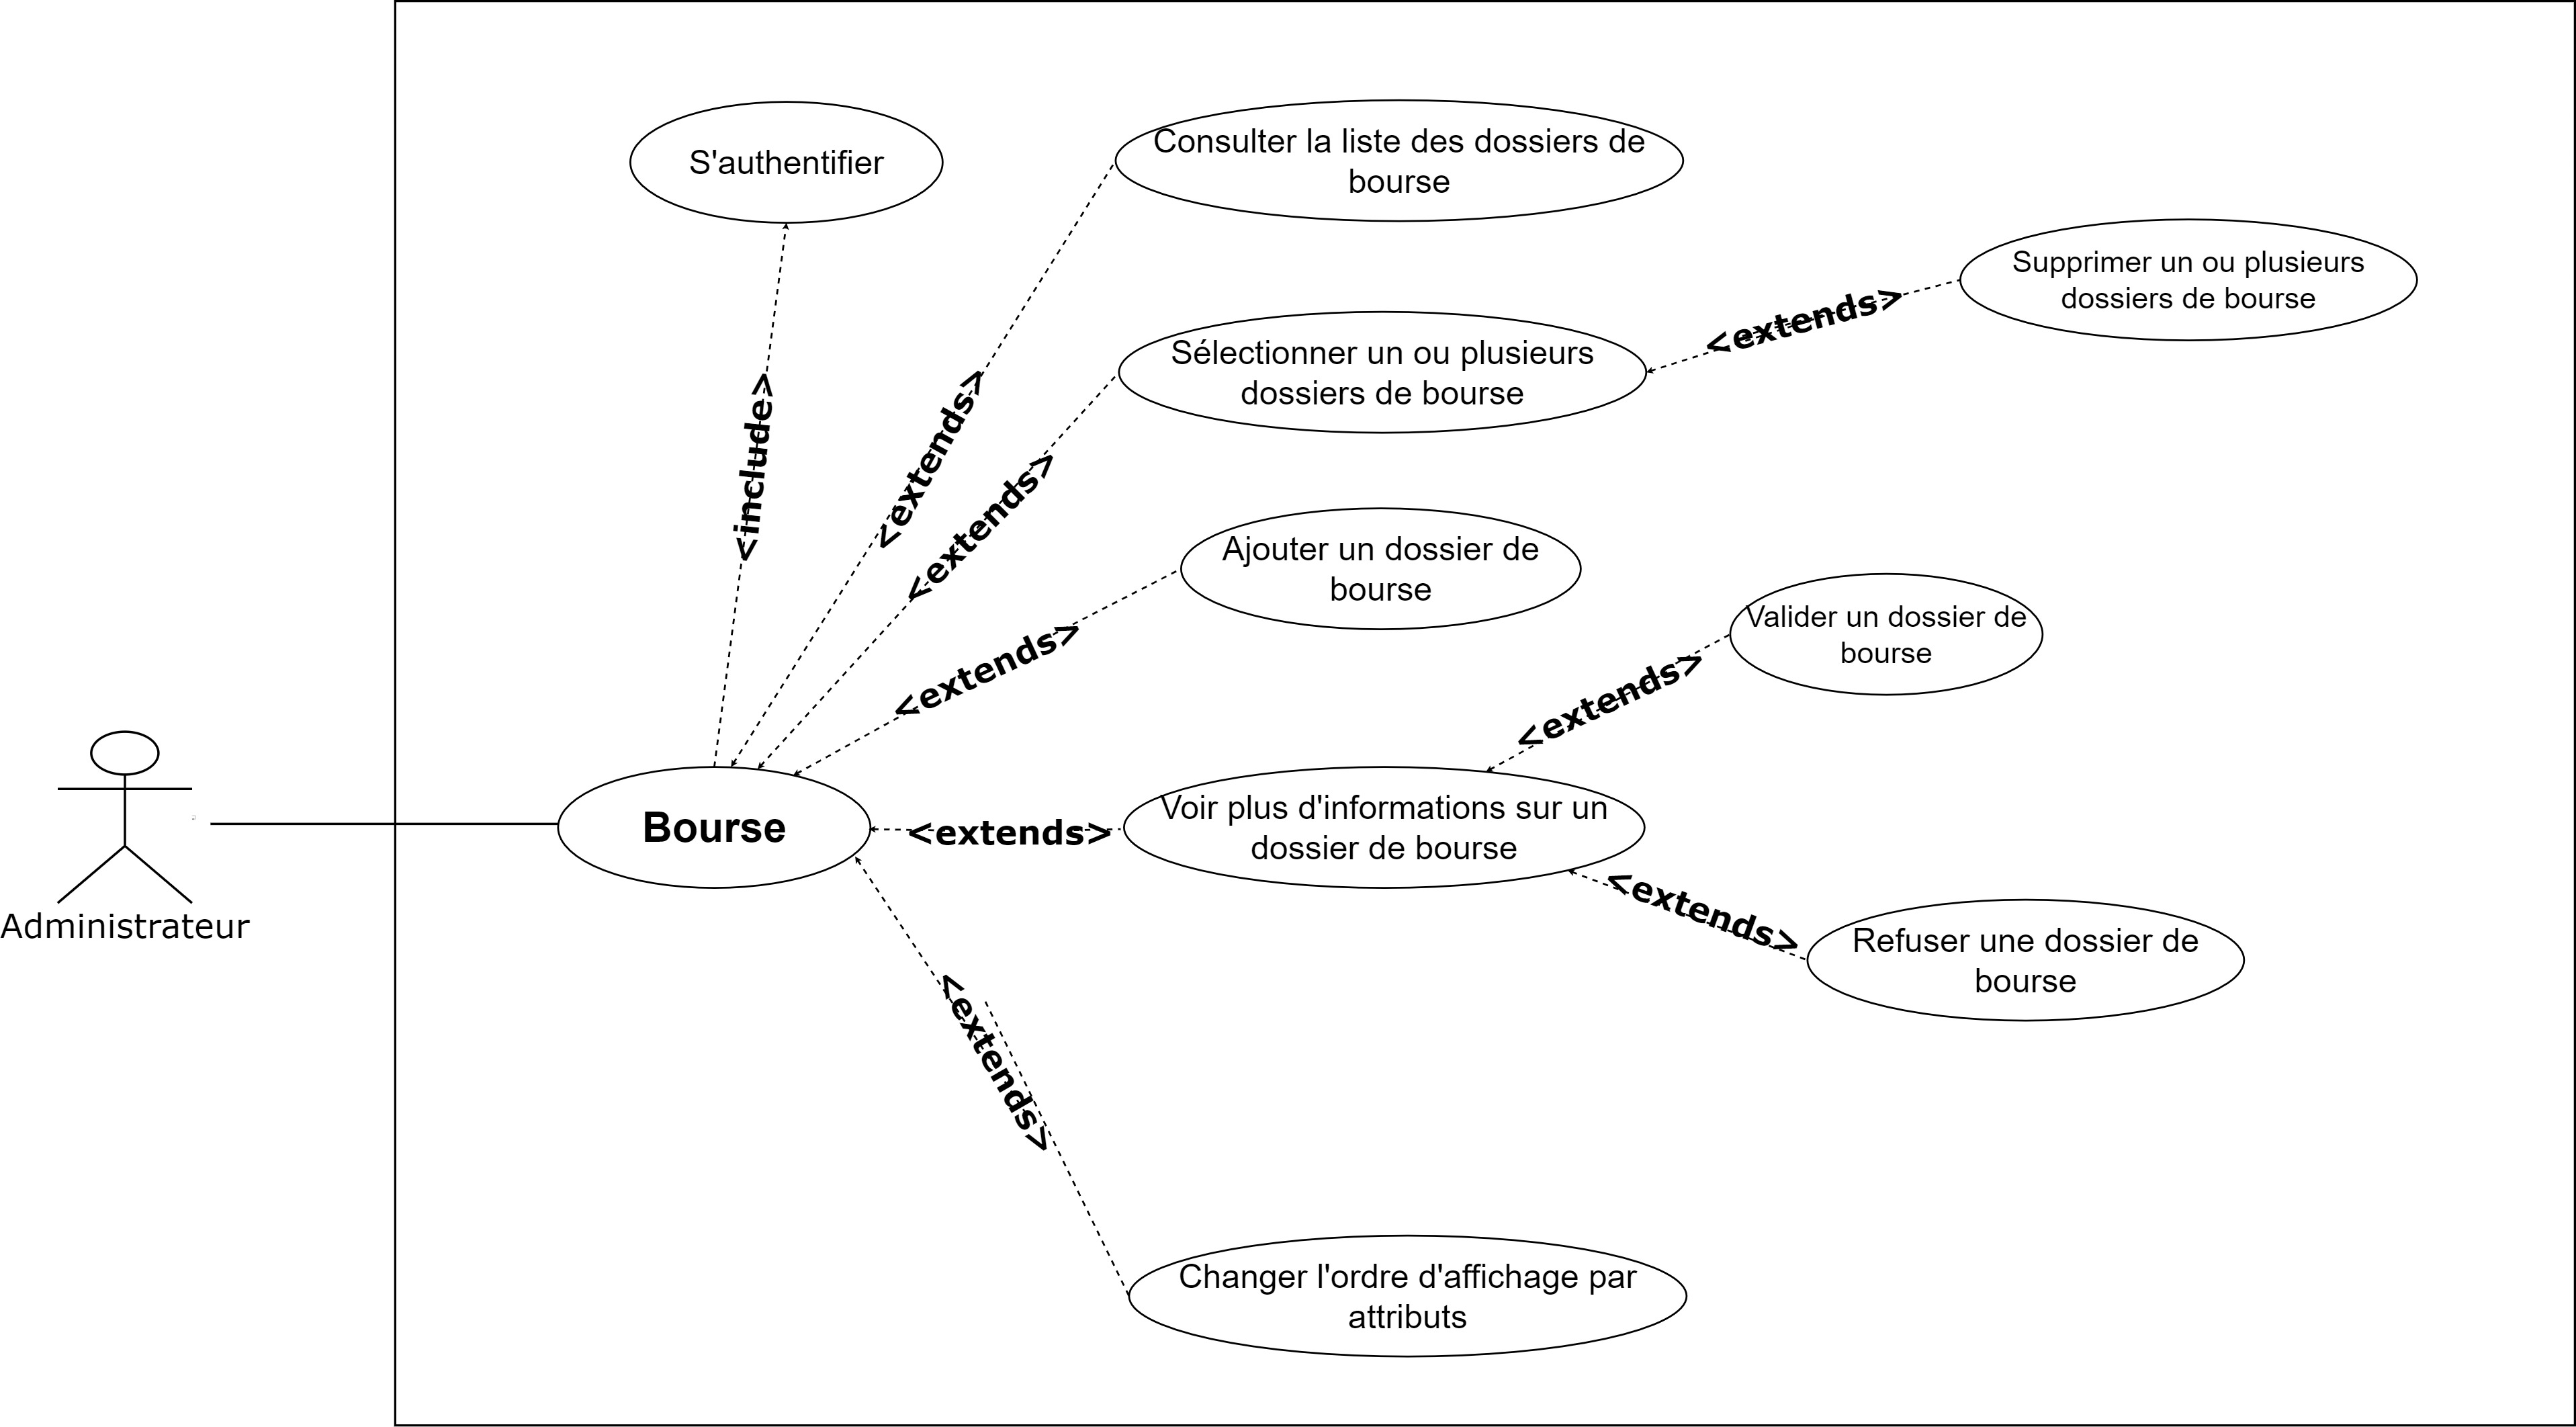
\includegraphics[scale=0.1]{ACR/Diagrammes/Bourse.jpg}
    \caption{Cas d'utilisation 'Bourses'}
\end{figure}

\subsubsection*{Cas d'utilisation 'Campus \& Résidences'}
\begin{figure}[H]
    \centering
    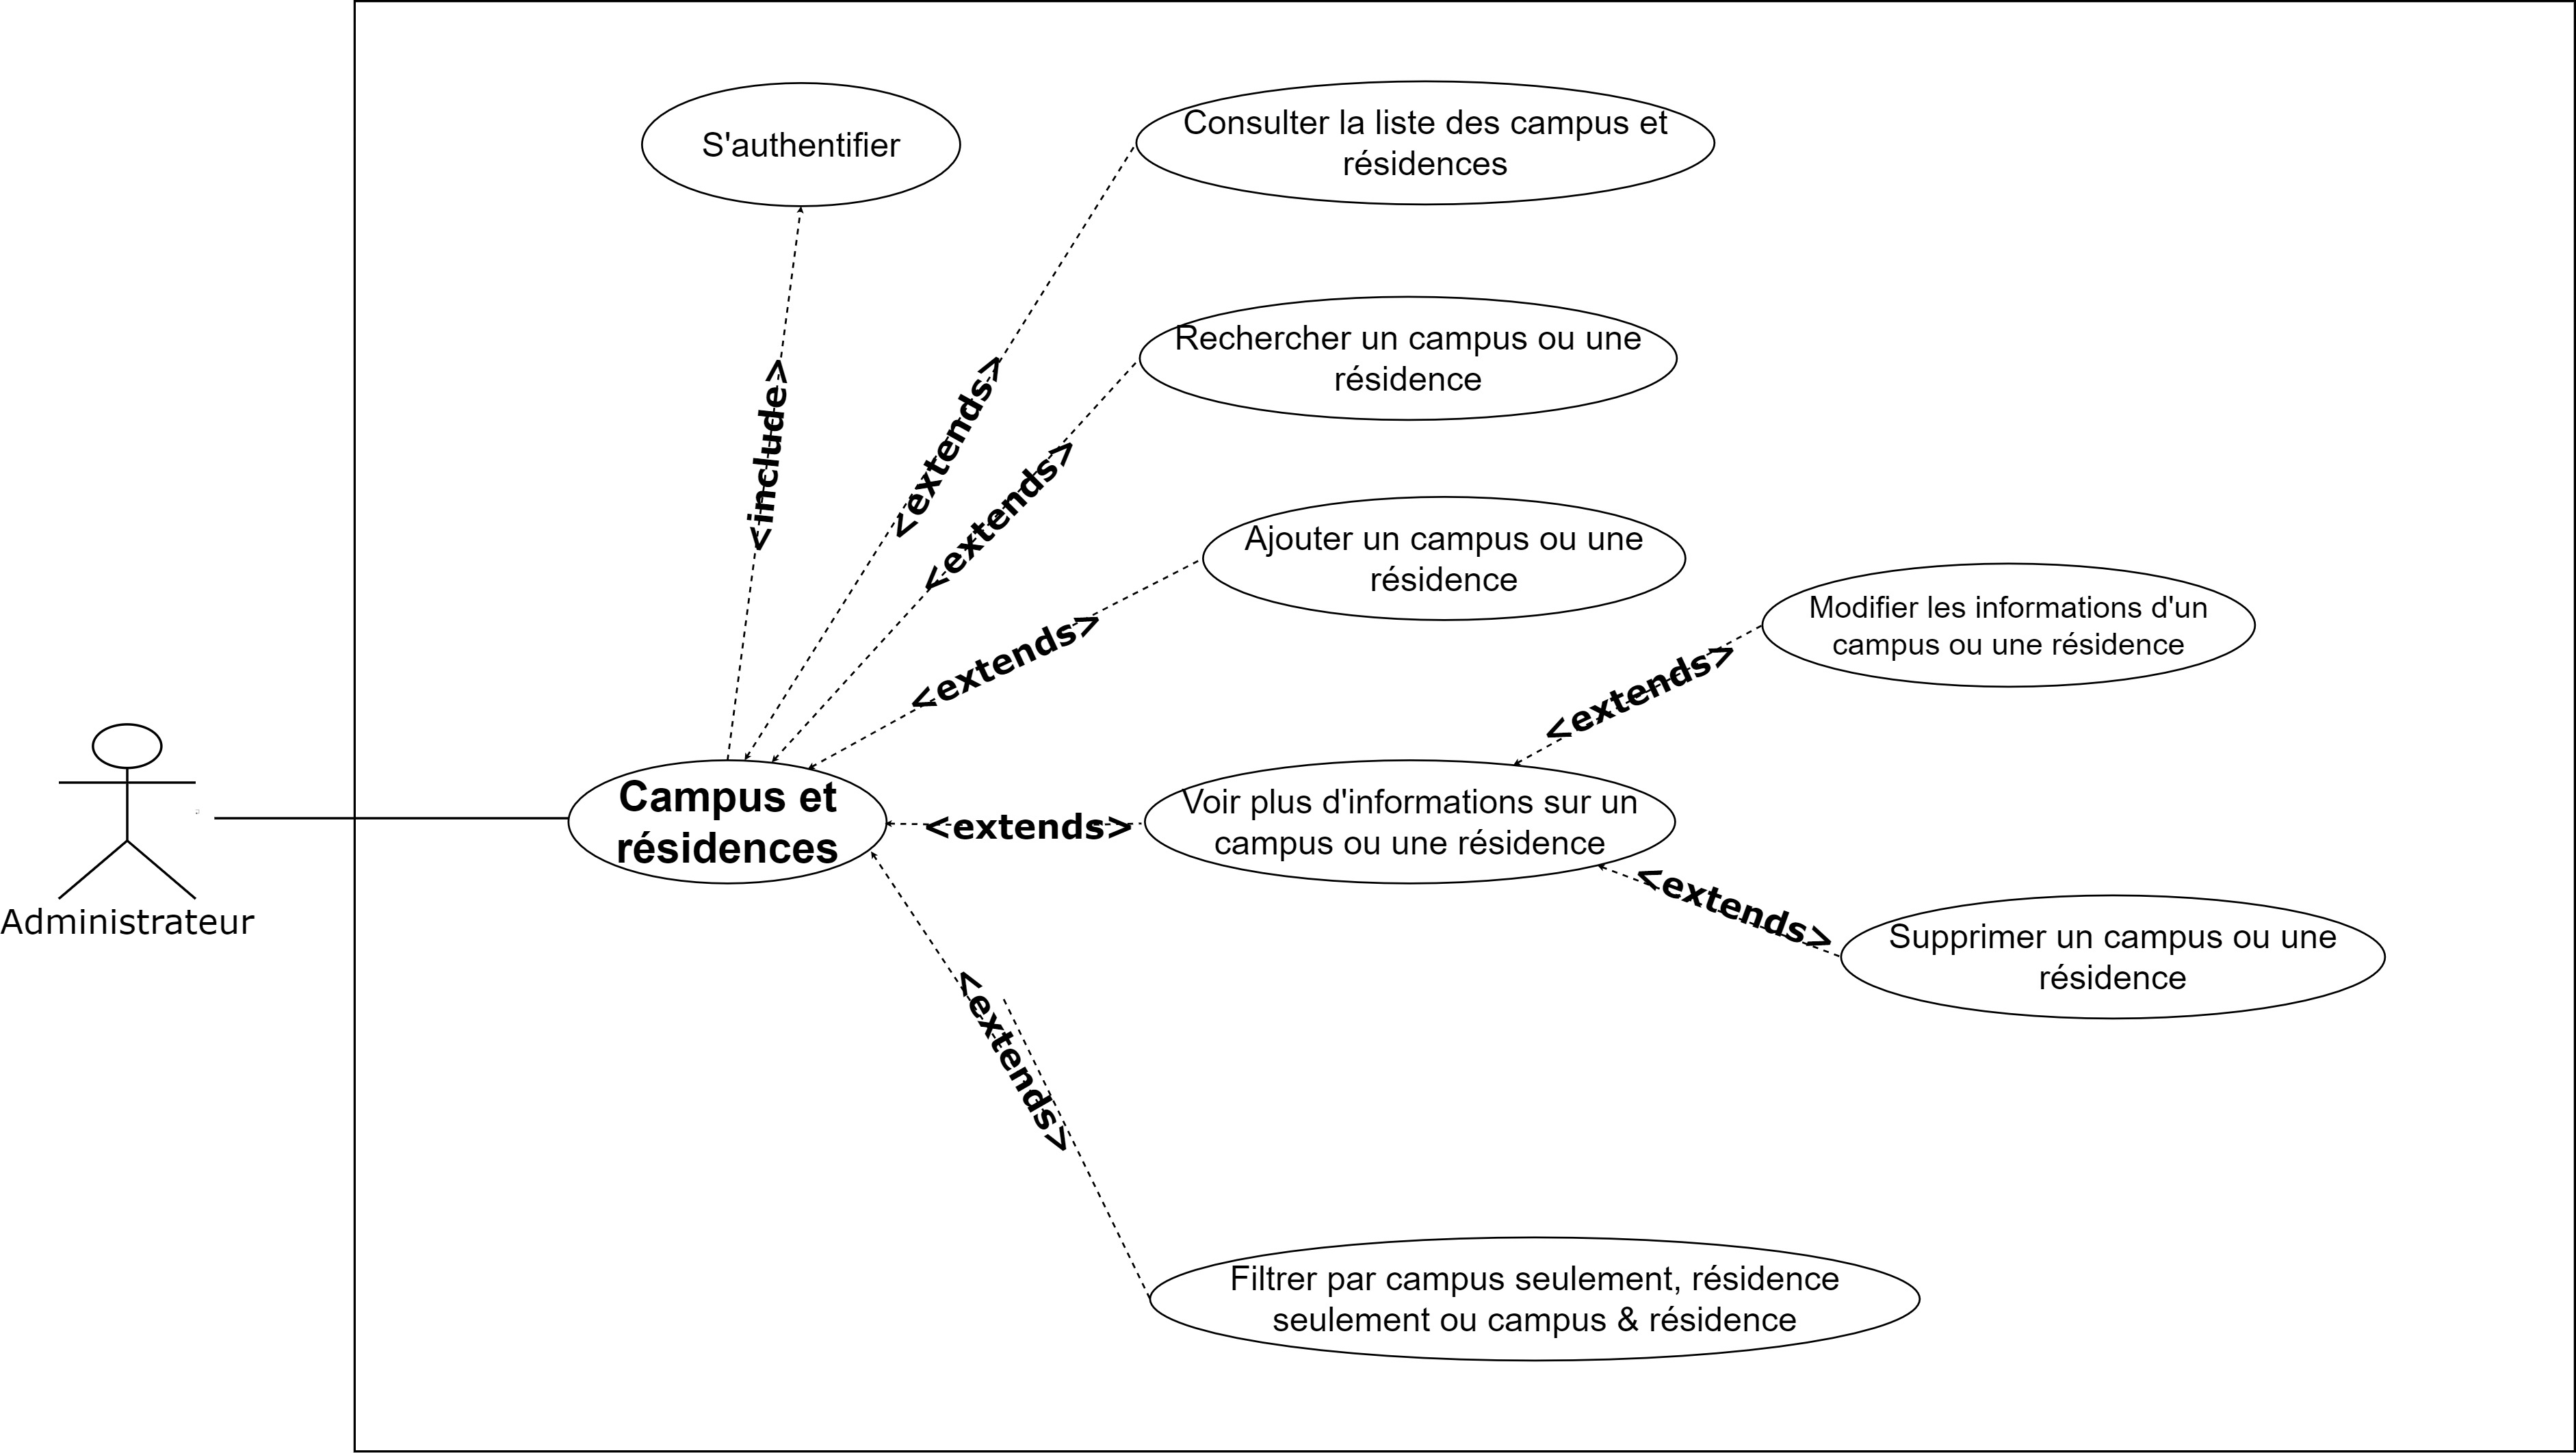
\includegraphics[scale=0.1]{ACR/Diagrammes/Campus-Residences.jpg}
    \caption{Cas d'utilisation 'Campus \& Résidences'}
\end{figure}

\subsubsection*{Cas d'utilisation 'Hébergement'}
\begin{figure}[H]
    \centering
    \includegraphics[scale=0.1]{ACR/Diagrammes/Hébergement.jpg}
    \caption{Cas d'utilisation 'Hébergement'}
\end{figure}

\subsubsection*{Cas d'utilisation 'Page d'accueil'}
\begin{figure}[H]
    \centering
    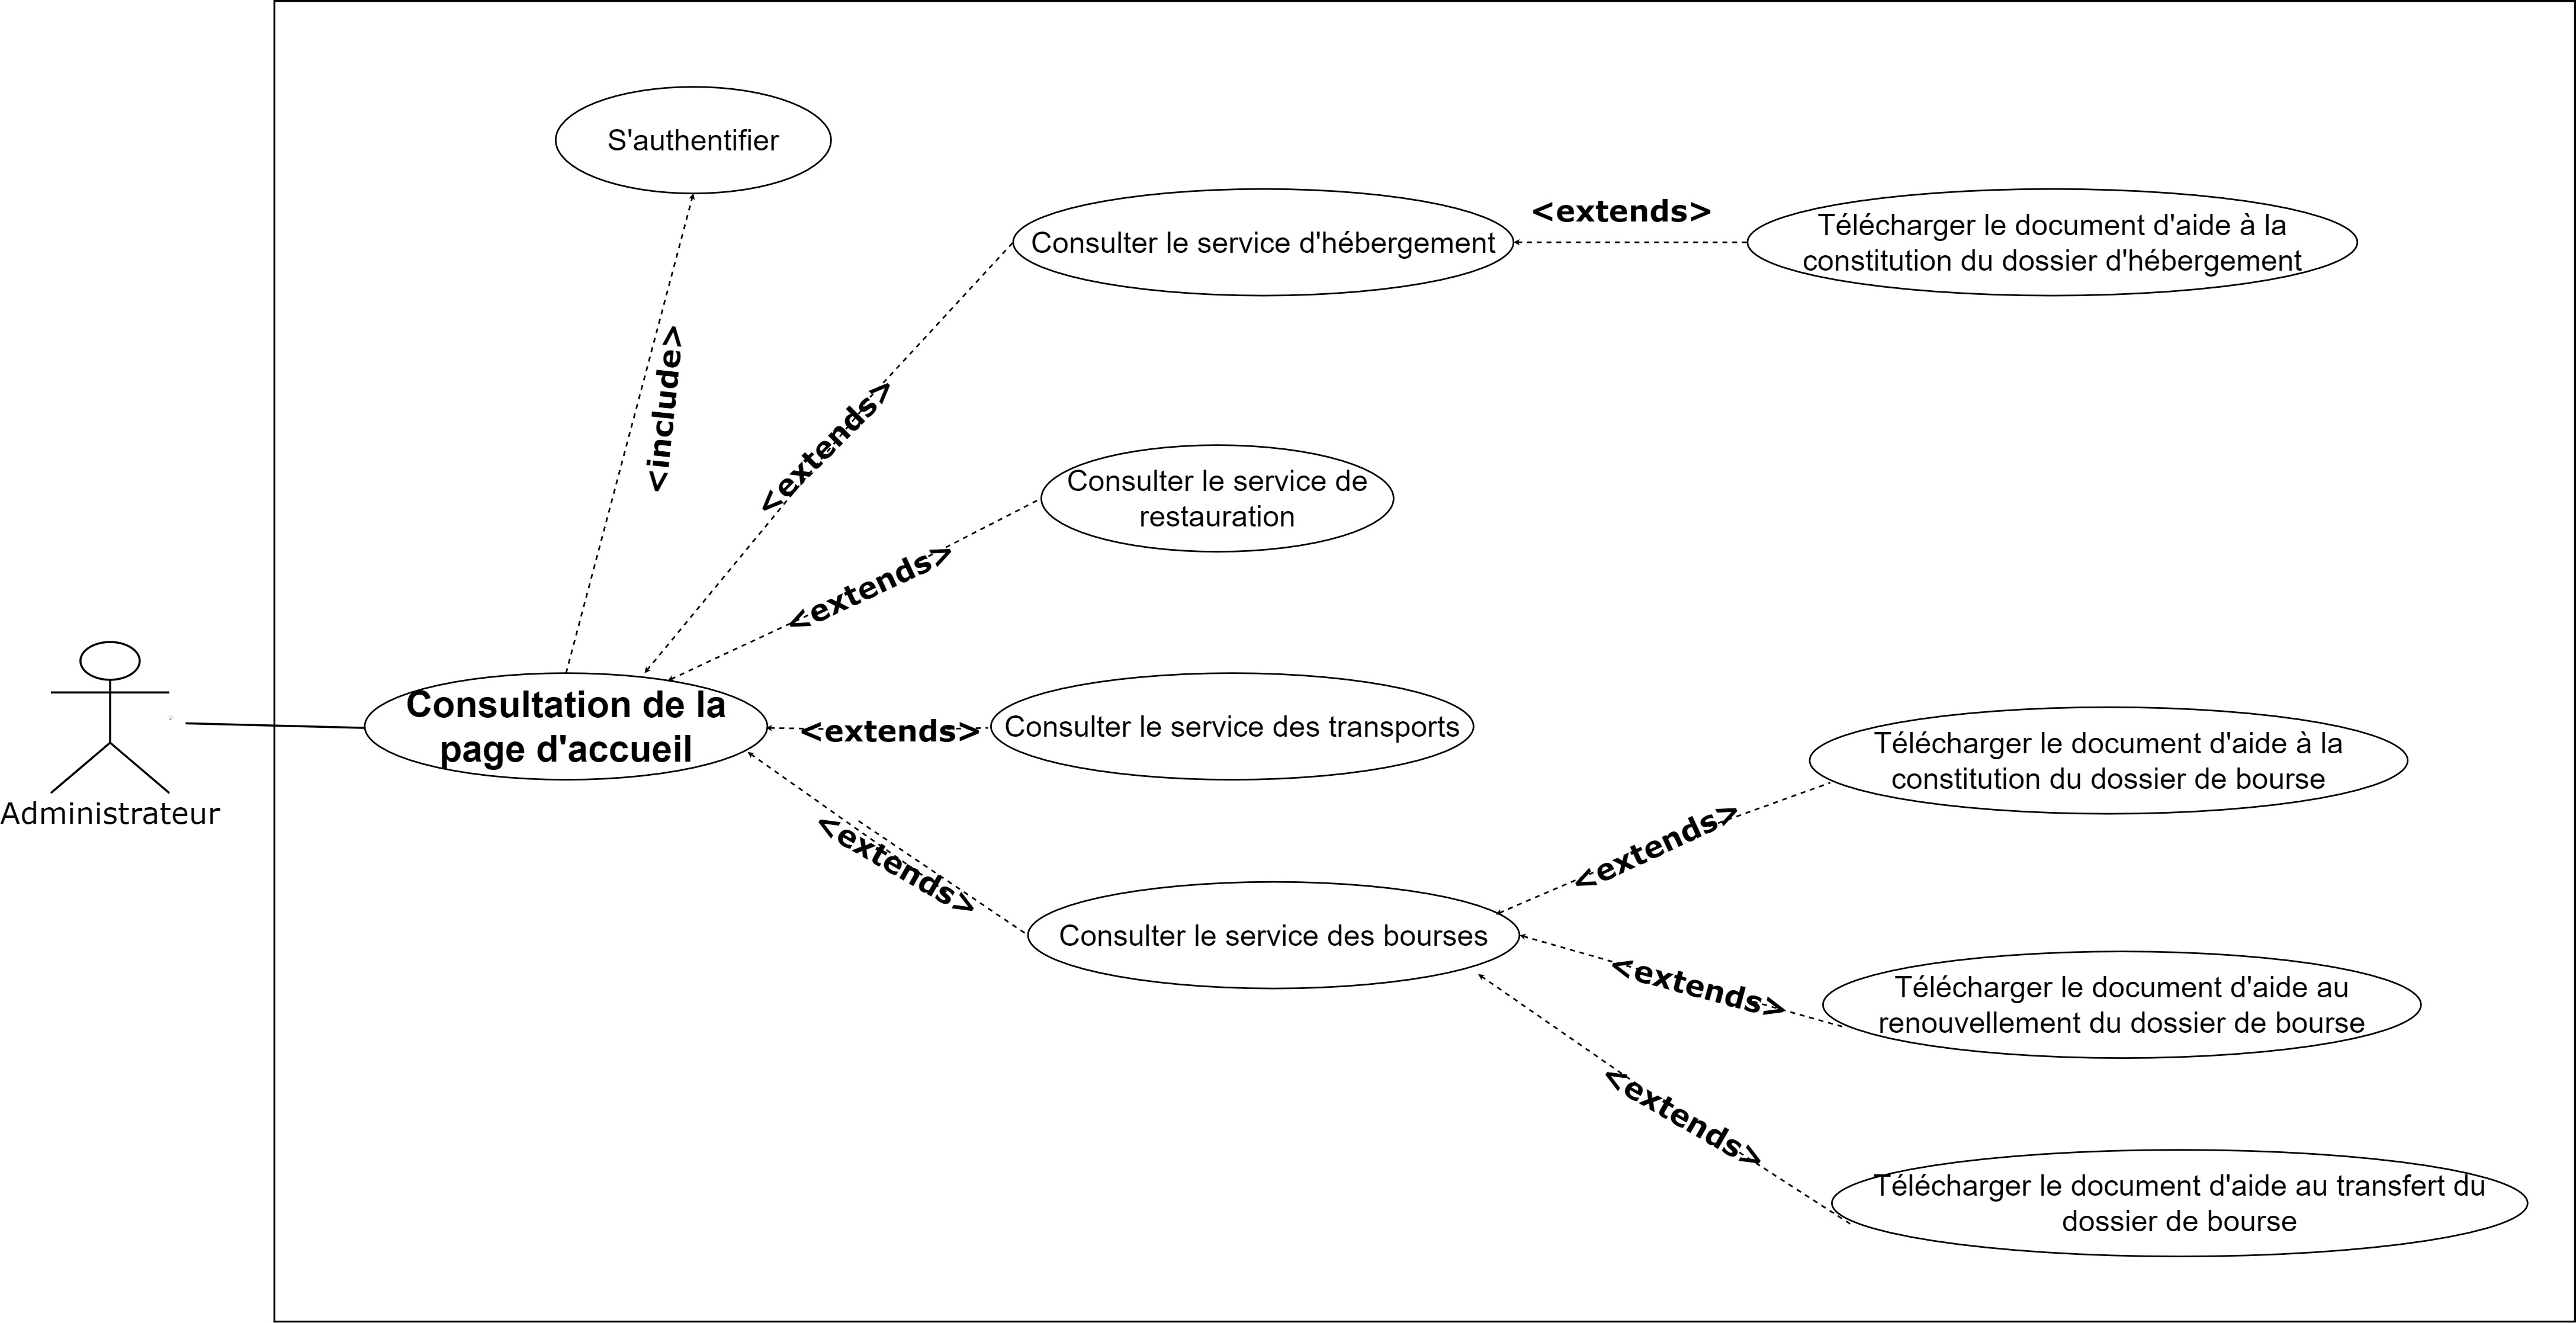
\includegraphics[scale=0.09]{ACR/Diagrammes/accueil.jpg}
    \caption{Cas d'utilisation 'Page d'accueil'}
\end{figure}

\subsubsection*{Cas d'utilisation 'Restauration - Calendrier'}
\begin{figure}[H]
    \centering
    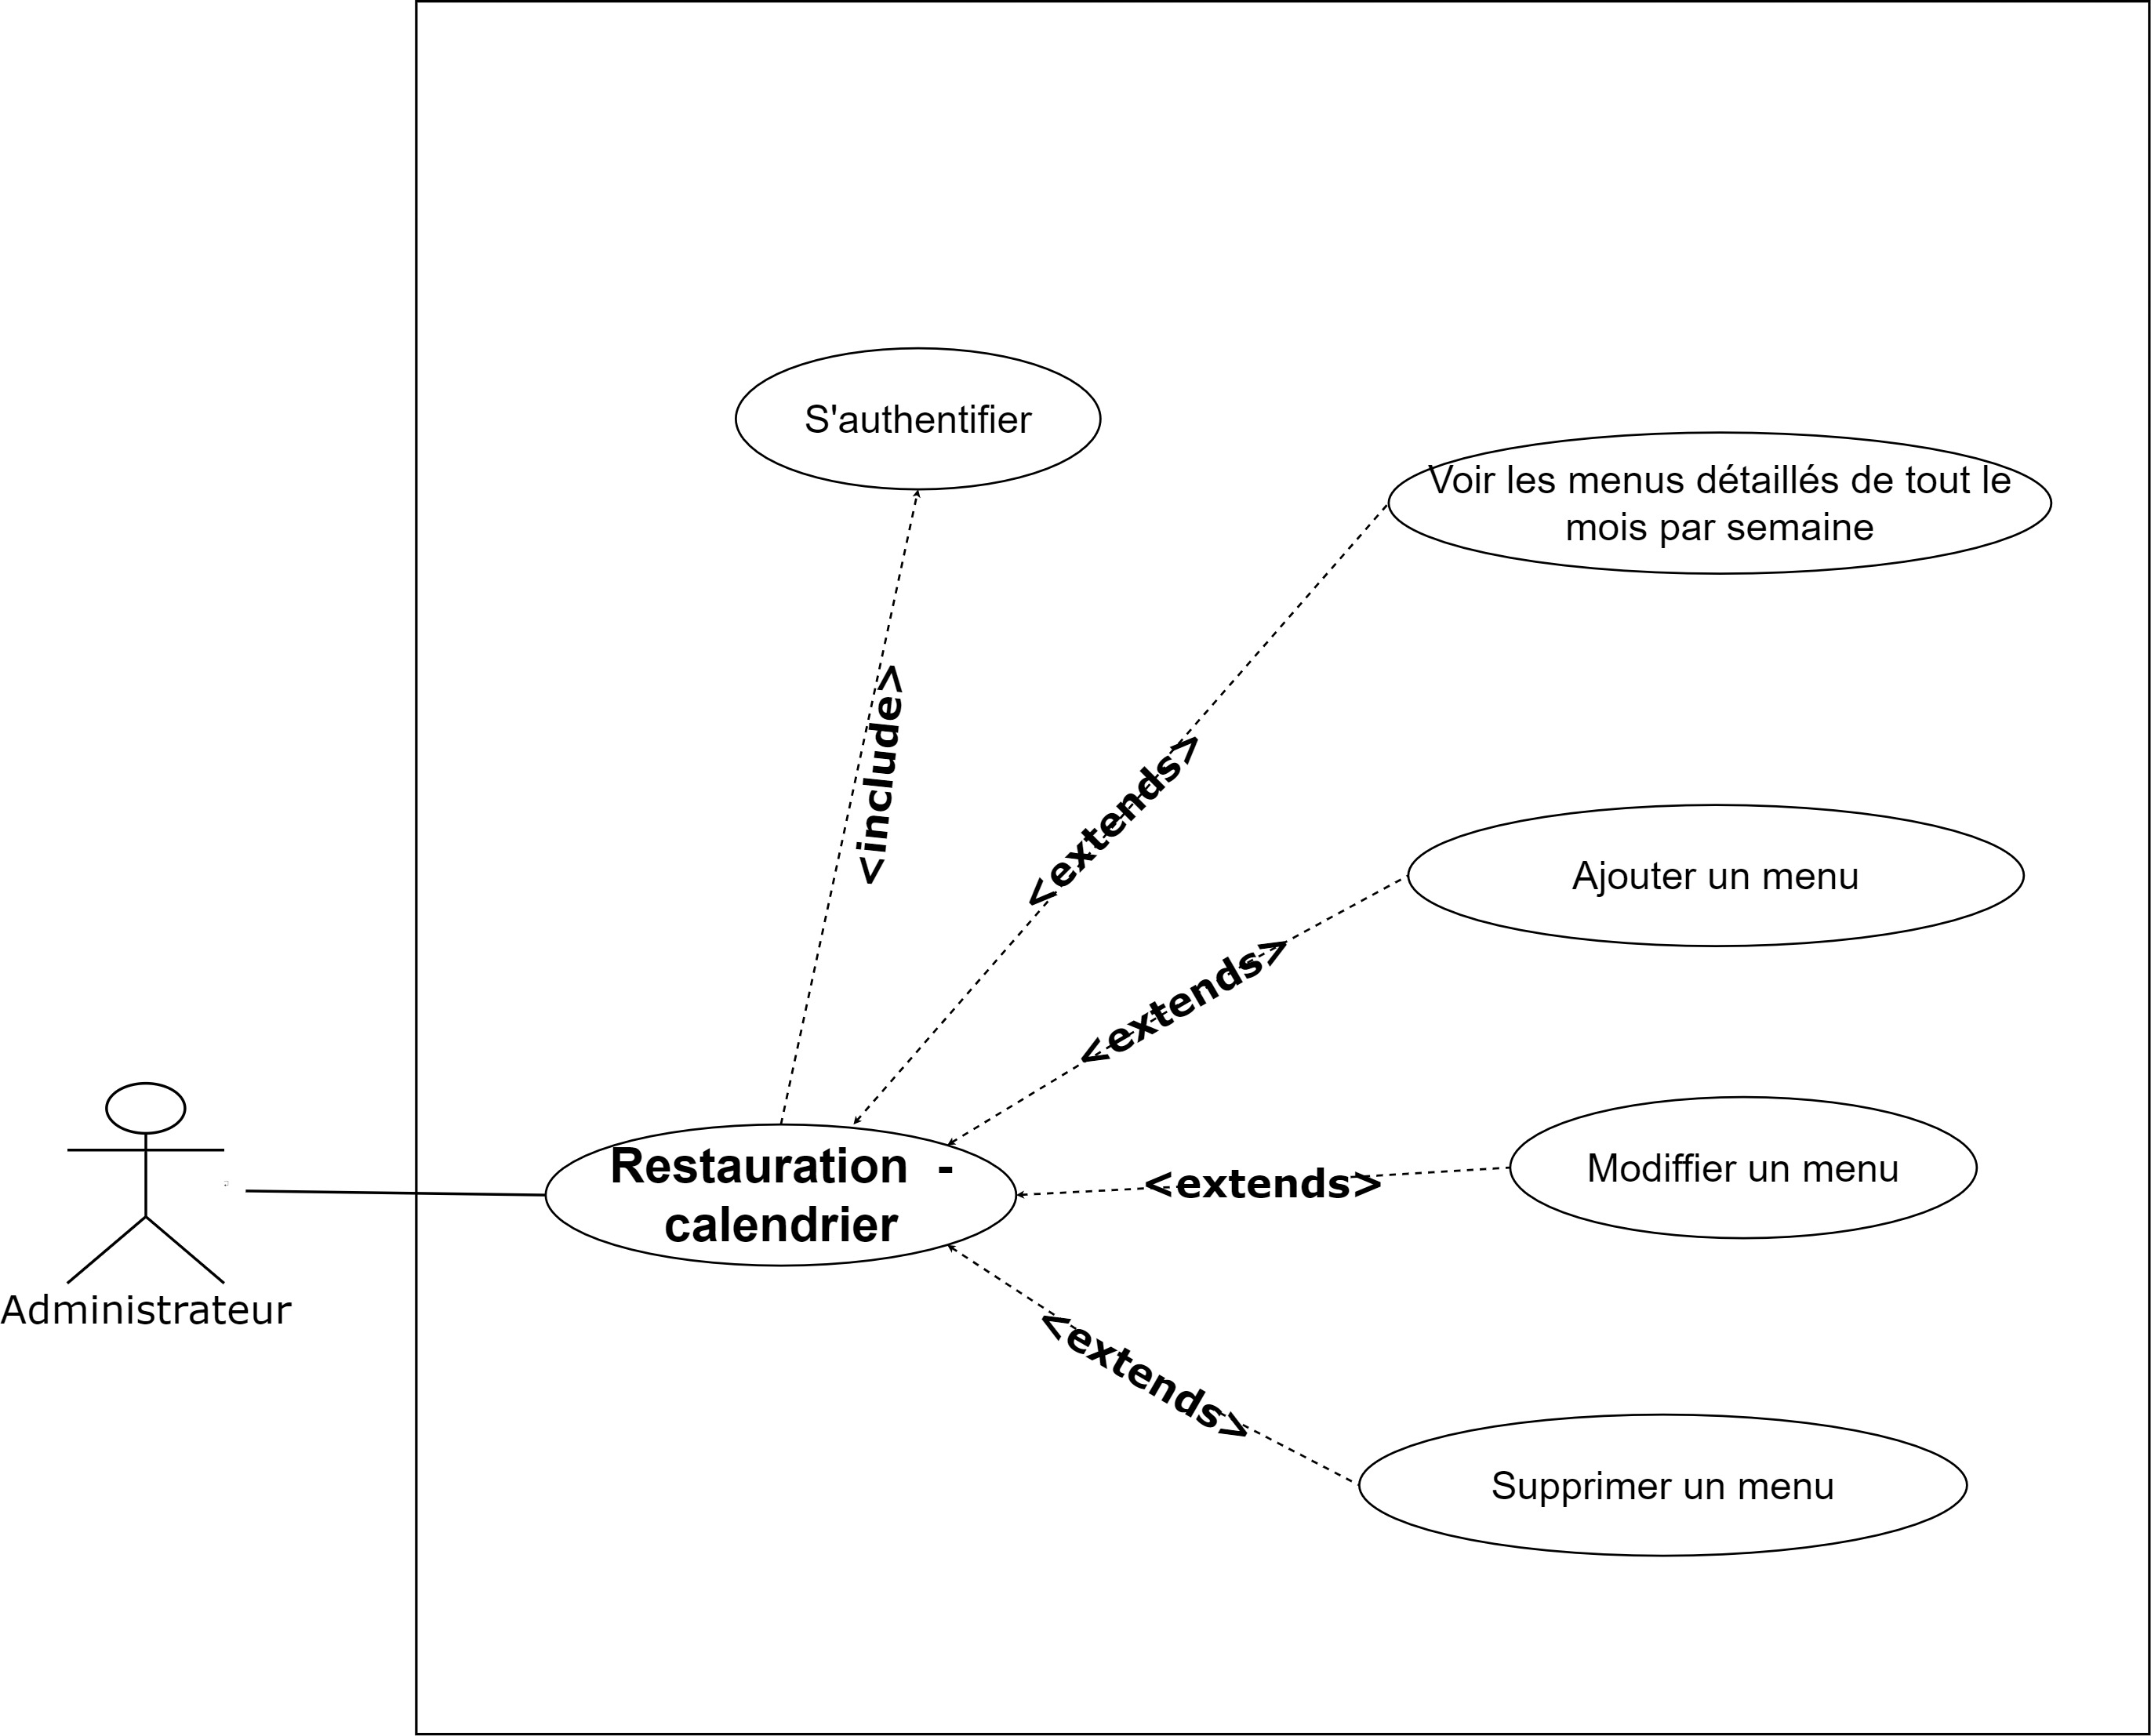
\includegraphics[scale=0.1]{ACR/Diagrammes/Restauration - calendrier.jpg}
    \caption{Cas d'utilisation 'Restauration - Calendrier'}
\end{figure}

\subsubsection*{Cas d'utilisation 'Restauration - Ingrédients'}
\begin{figure}[H]
    \centering
    \includegraphics[scale=0.1]{ACR/Diagrammes/Restauration - ingrédients.jpg}
    \caption{Cas d'utilisation 'Restauration - Ingrédients'}
\end{figure}

\subsubsection*{Cas d'utilisation 'Restauration - Plats \& Desserts'}
\begin{figure}[H]
    \centering
    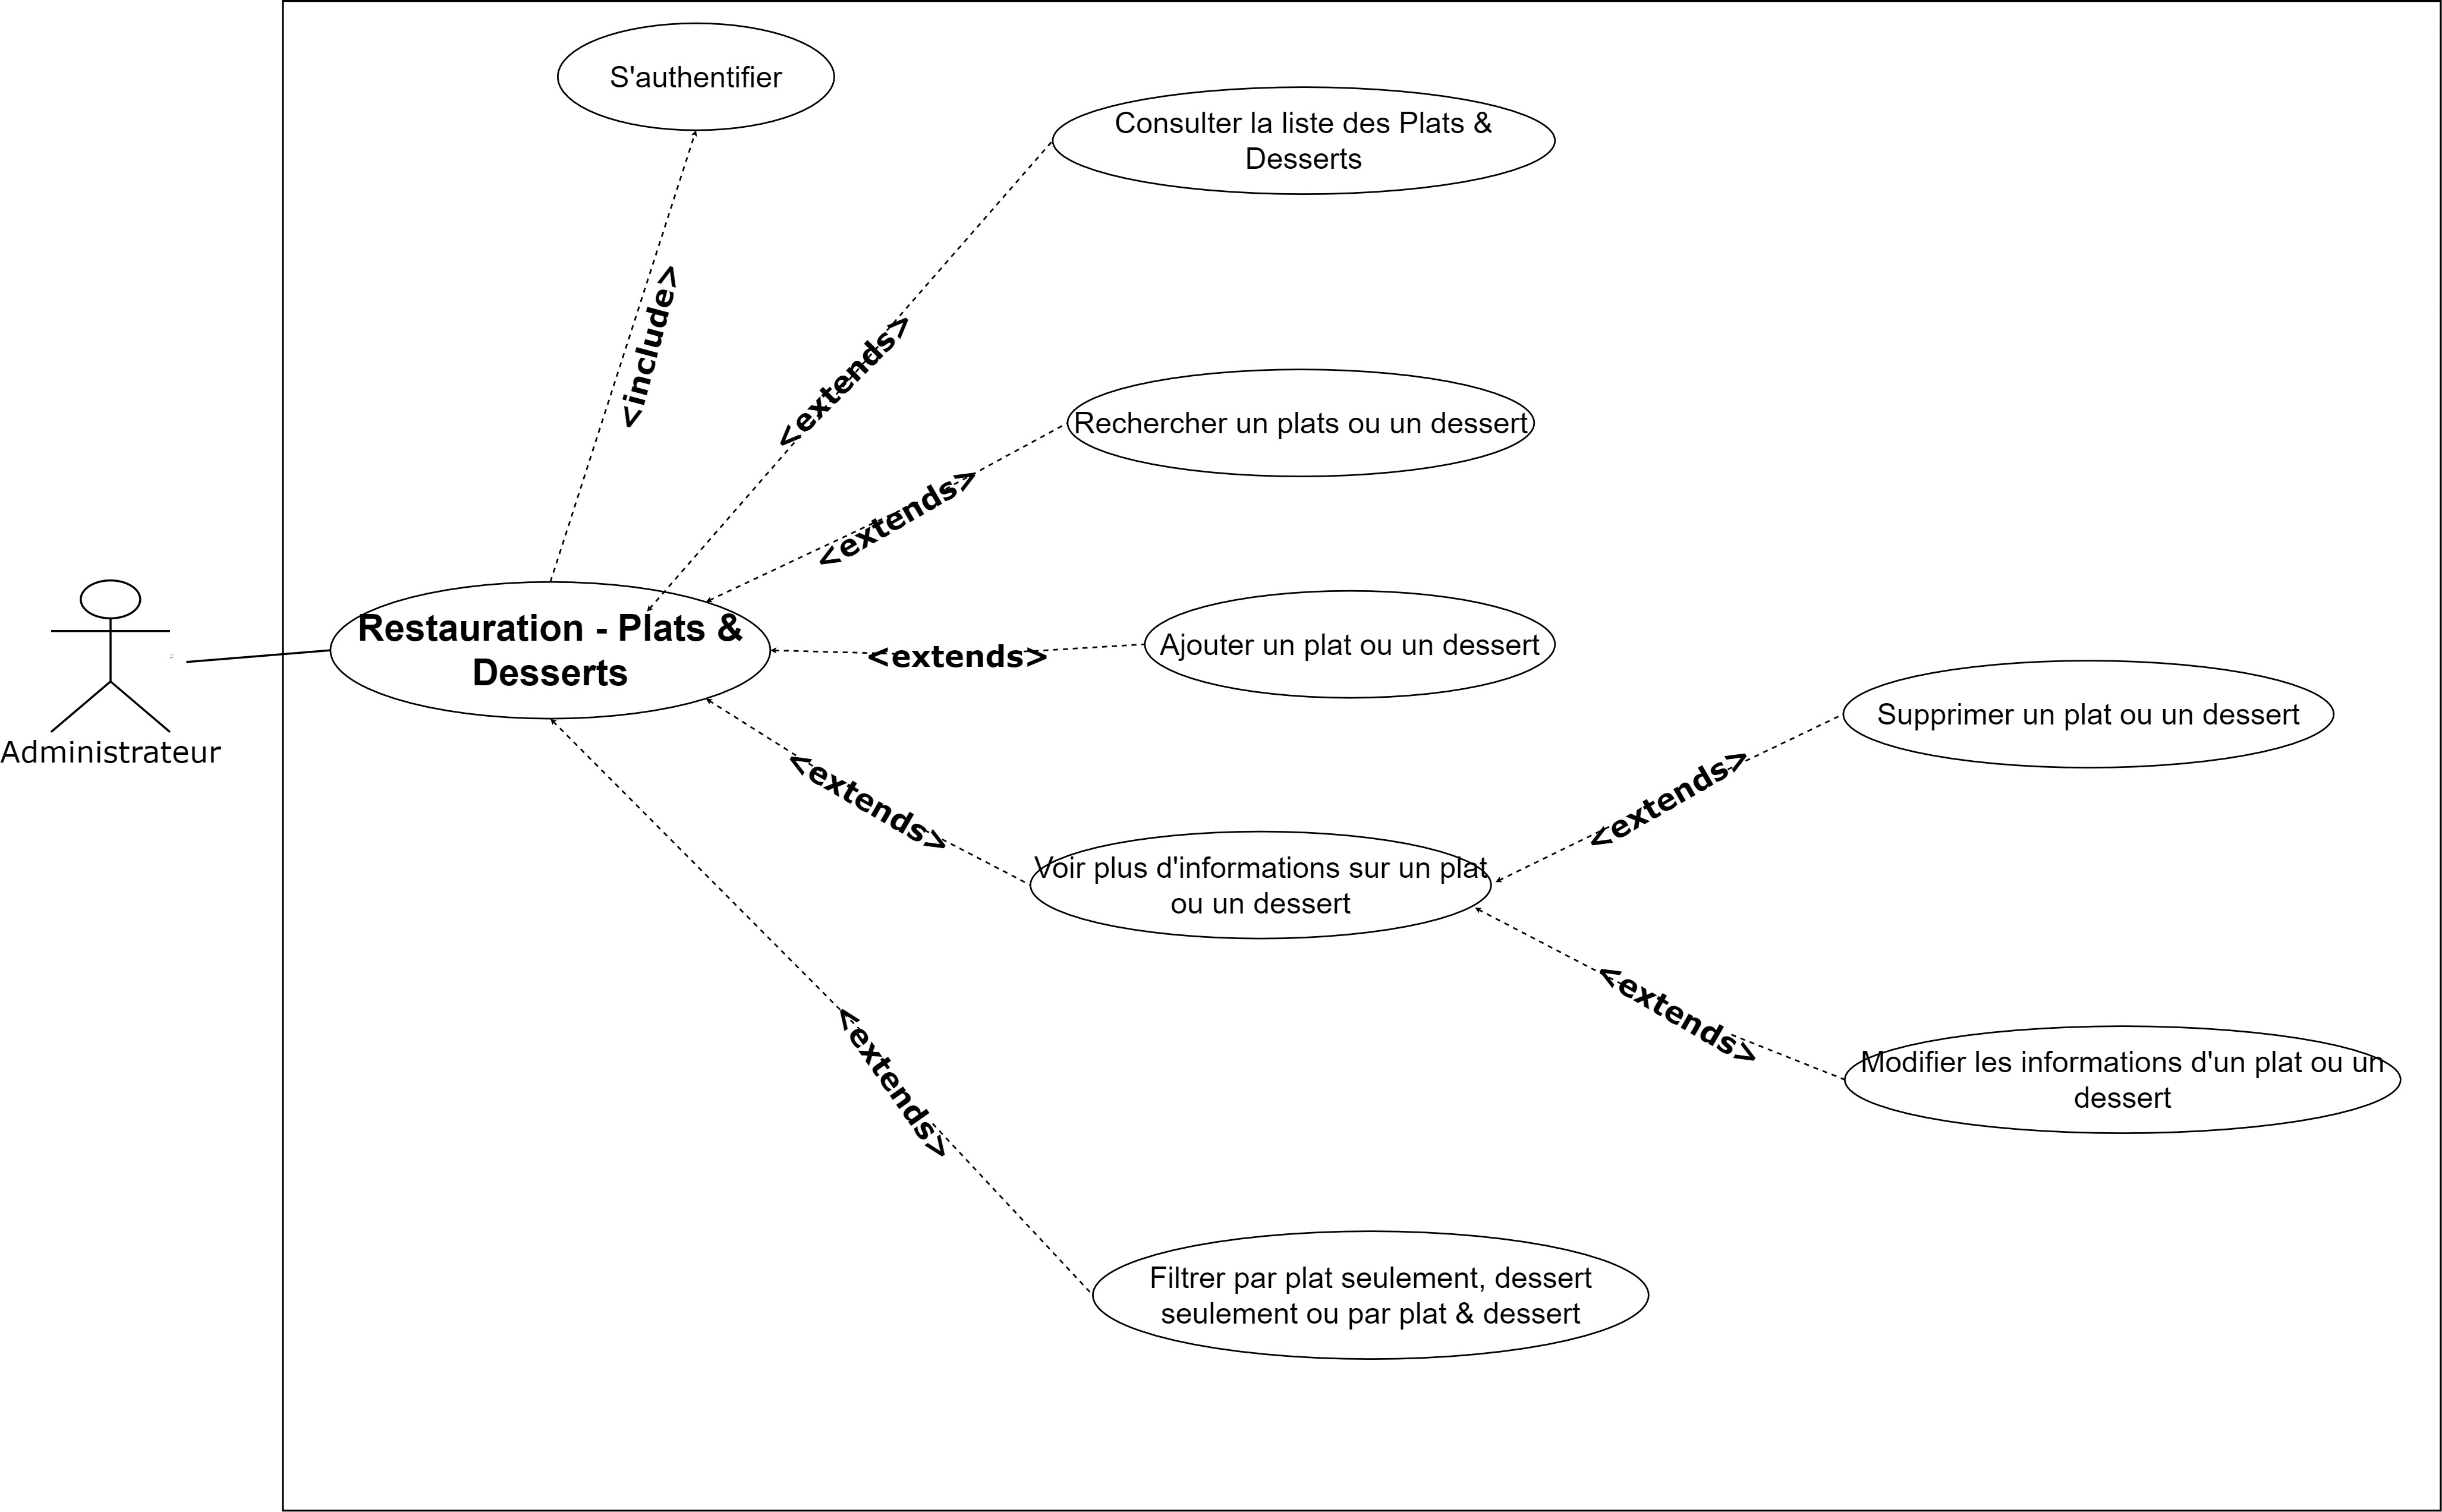
\includegraphics[scale=0.1]{ACR/Diagrammes/Restauration - Plats&Desserts.jpg}
    \caption{Cas d'utilisation 'Restauration - Plats \& Desserts'}
\end{figure}

\subsubsection*{Cas d'utilisation 'Restauration - Restaurants'}
\begin{figure}[H]
    \centering
    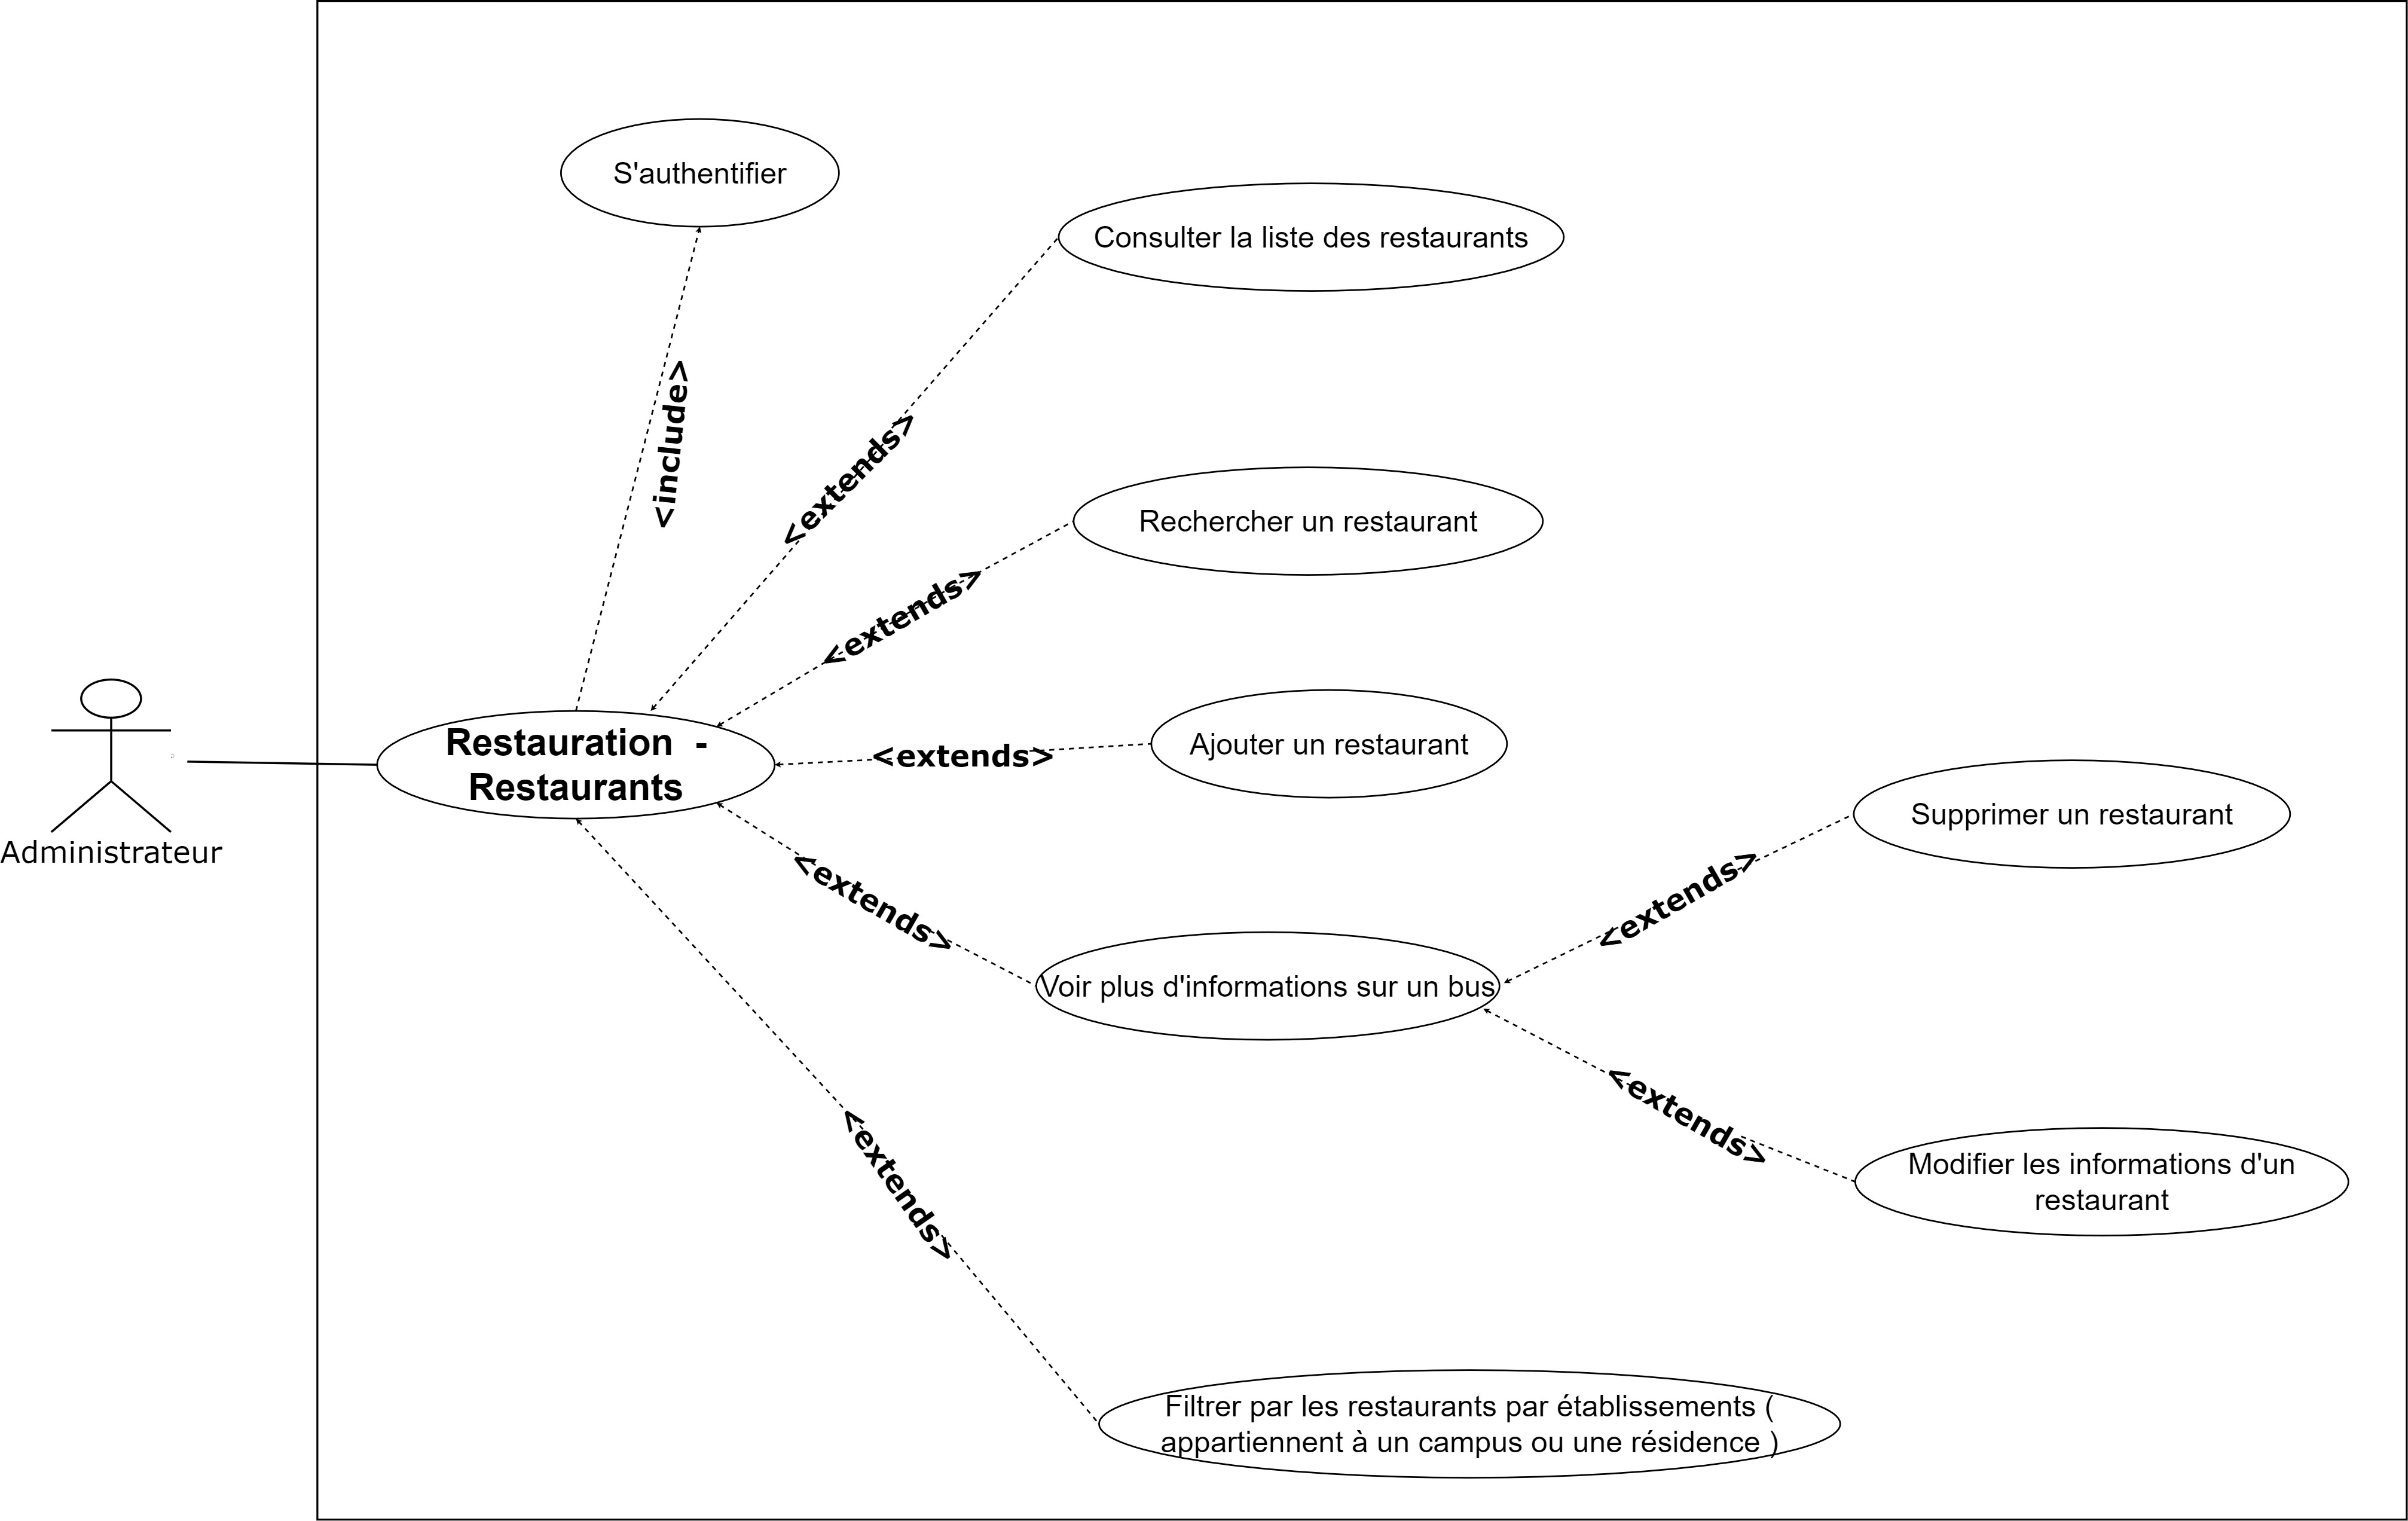
\includegraphics[scale=0.1]{ACR/Diagrammes/Restauration - restaurants.jpg}
    \caption{Cas d'utilisation 'Restauration - Restaurants'}
\end{figure}

\subsubsection*{Cas d'utilisation 'Transports - Bus'}
\begin{figure}[H]
    \centering
    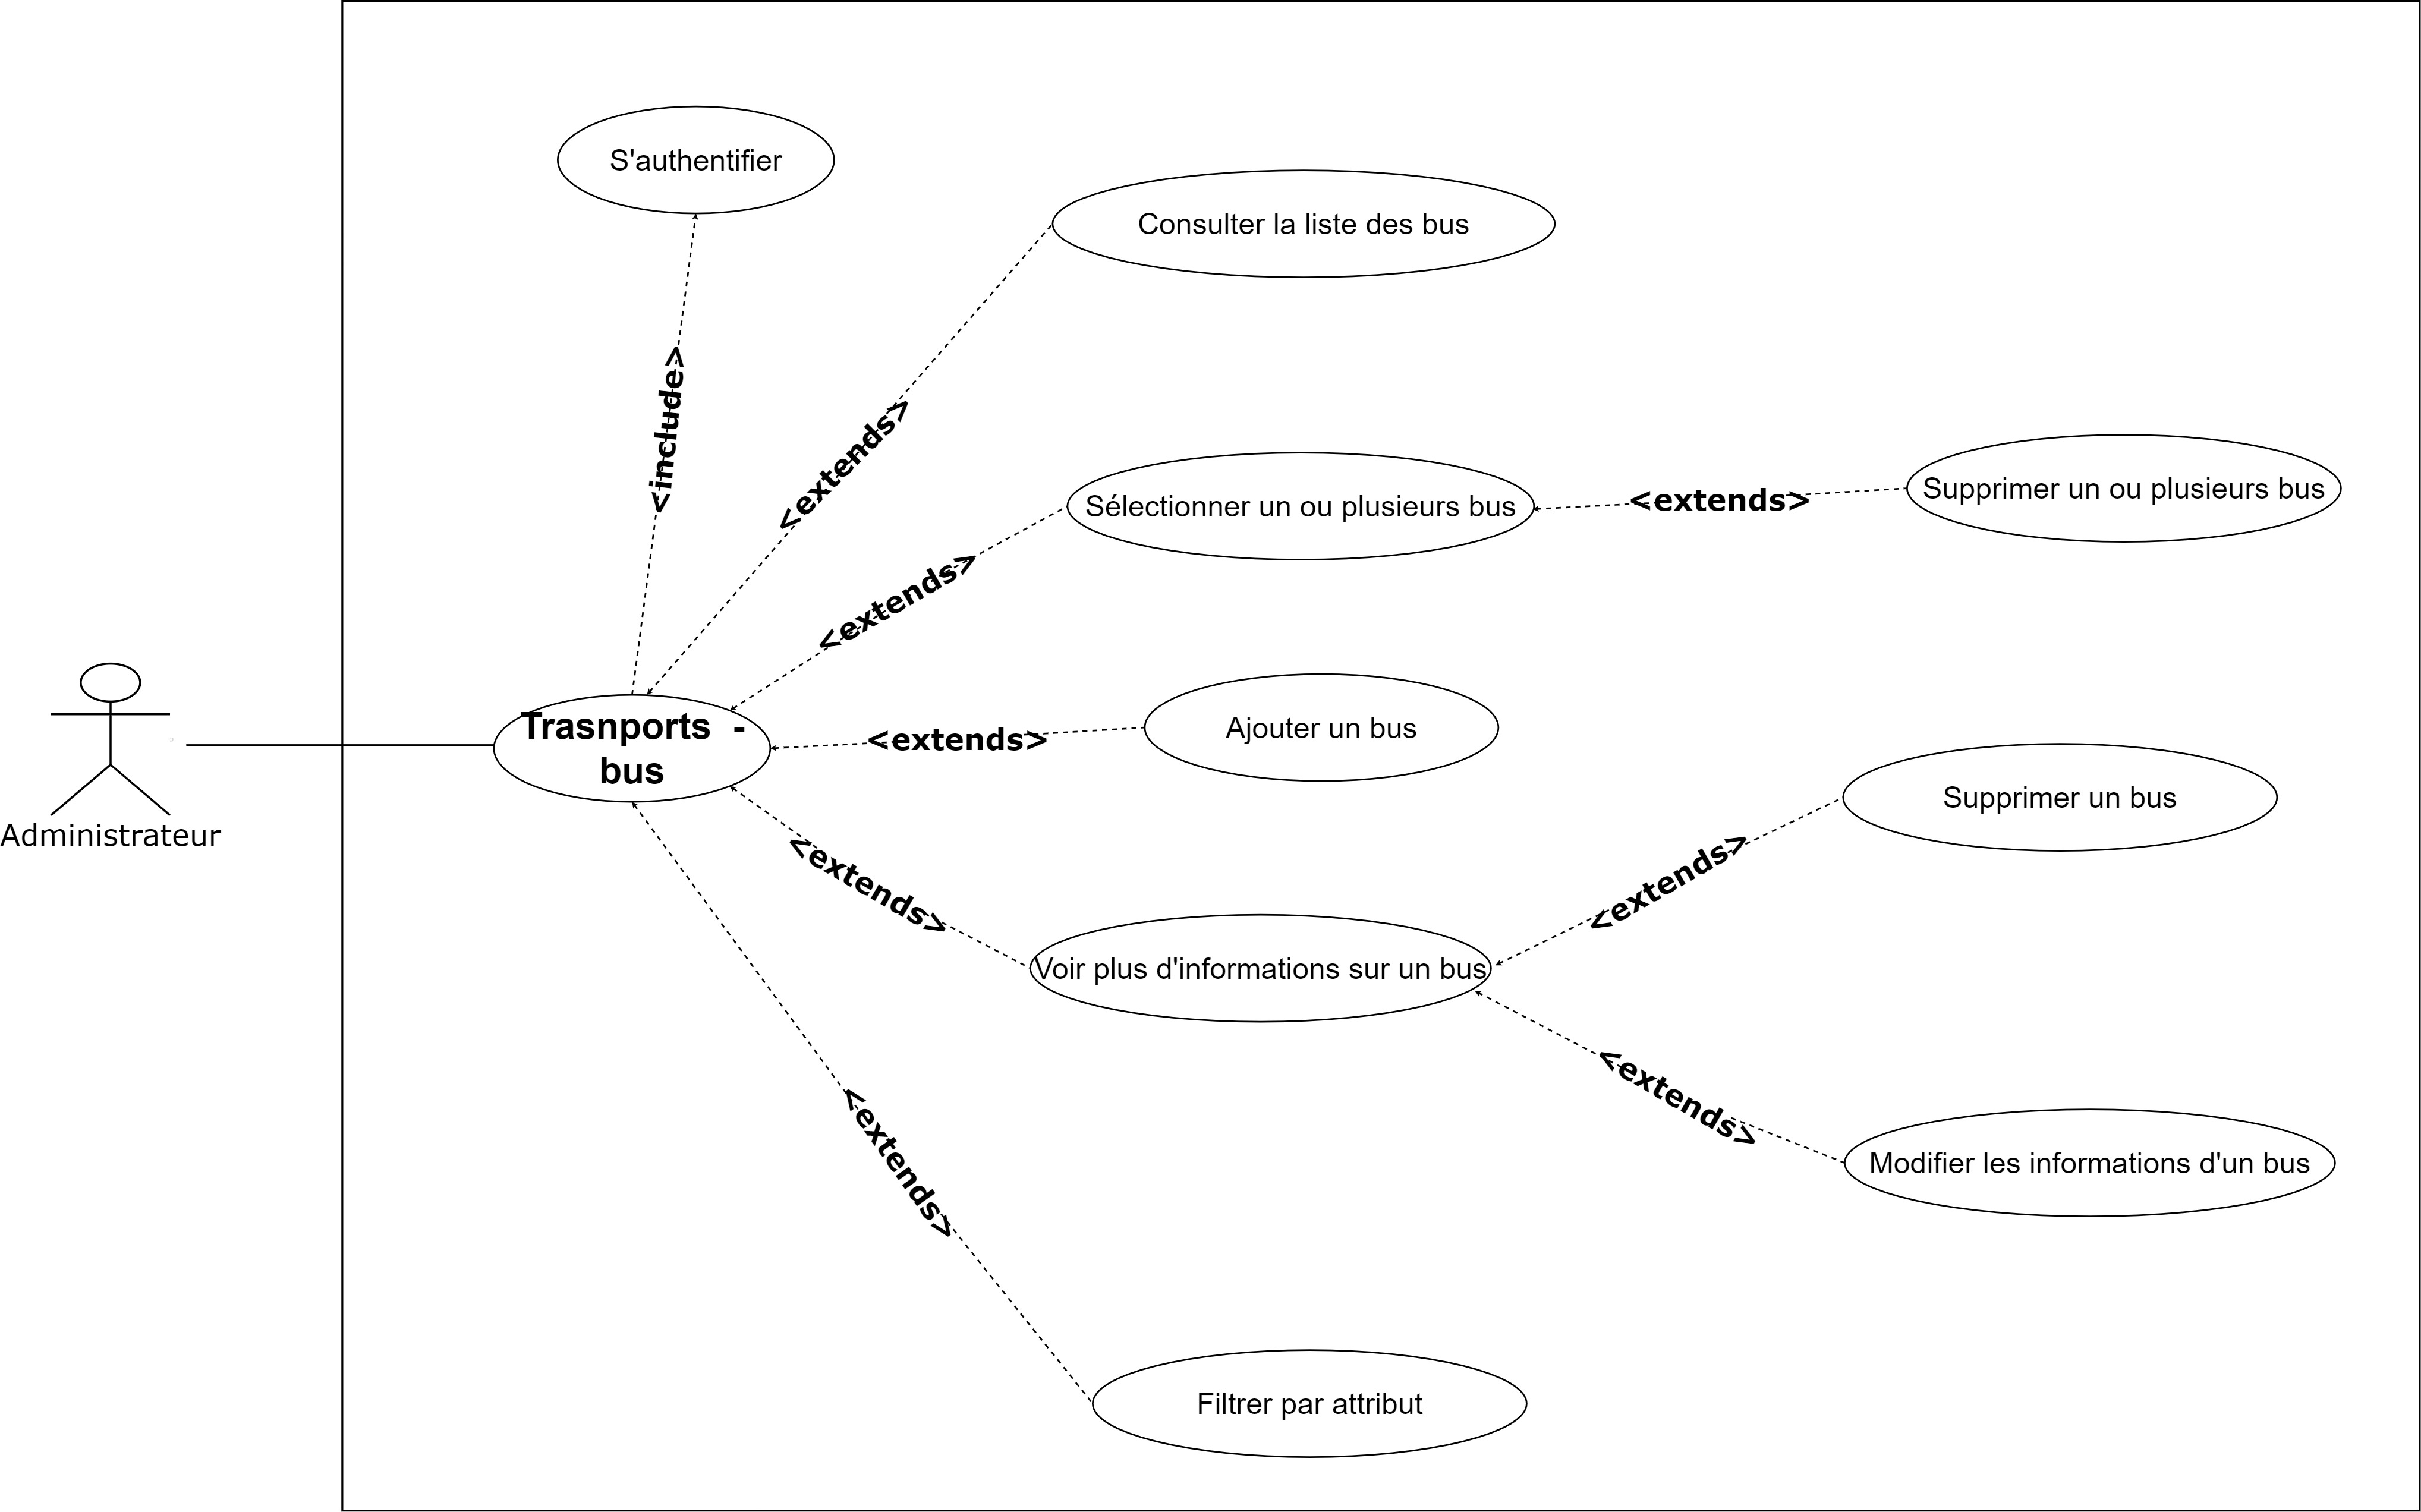
\includegraphics[scale=0.1]{ACR/Diagrammes/Transports - bus.jpg}
    \caption{Cas d'utilisation 'Transports - Bus'}
\end{figure}

\subsubsection*{Cas d'utilisation 'Transports - Calendrier'}
\begin{figure}[H]
    \centering
    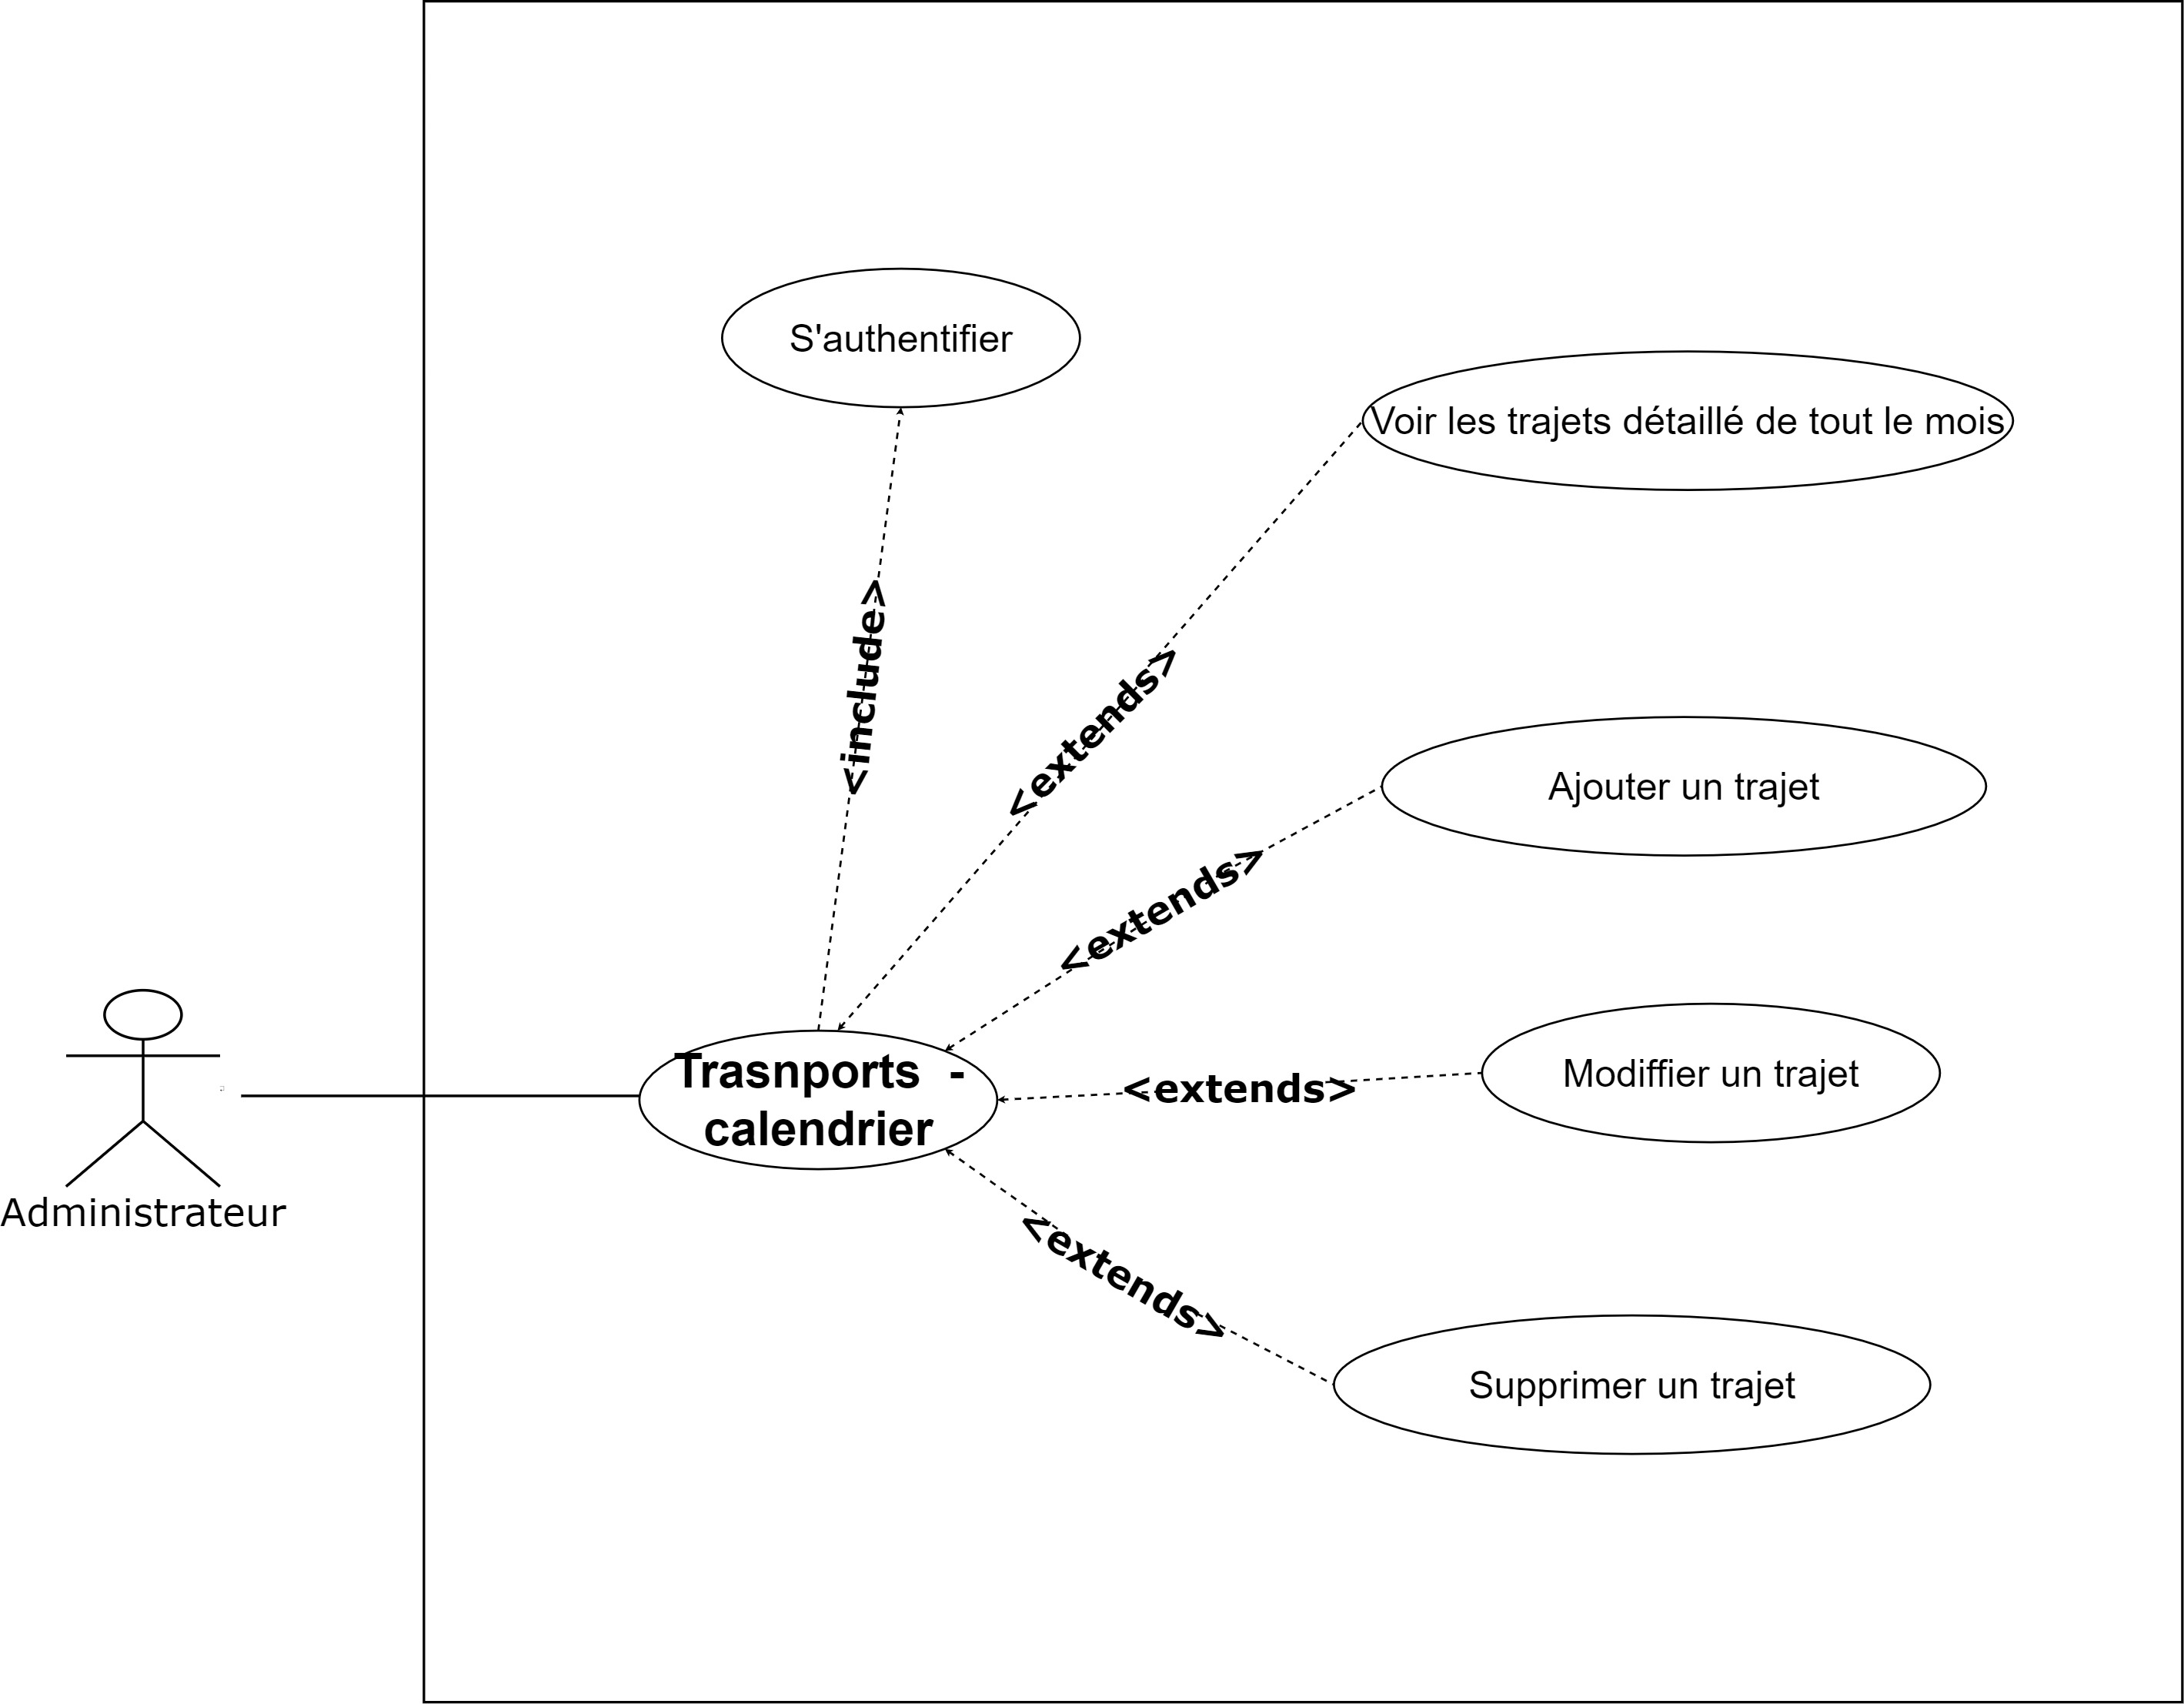
\includegraphics[scale=0.1]{ACR/Diagrammes/Transports - calendrier.jpg}
    \caption{Cas d'utilisation 'Transports - Calendrier'}
\end{figure}

\subsubsection*{Cas d'utilisation 'Utilisateurs'}
\begin{figure}[H]
    \centering
    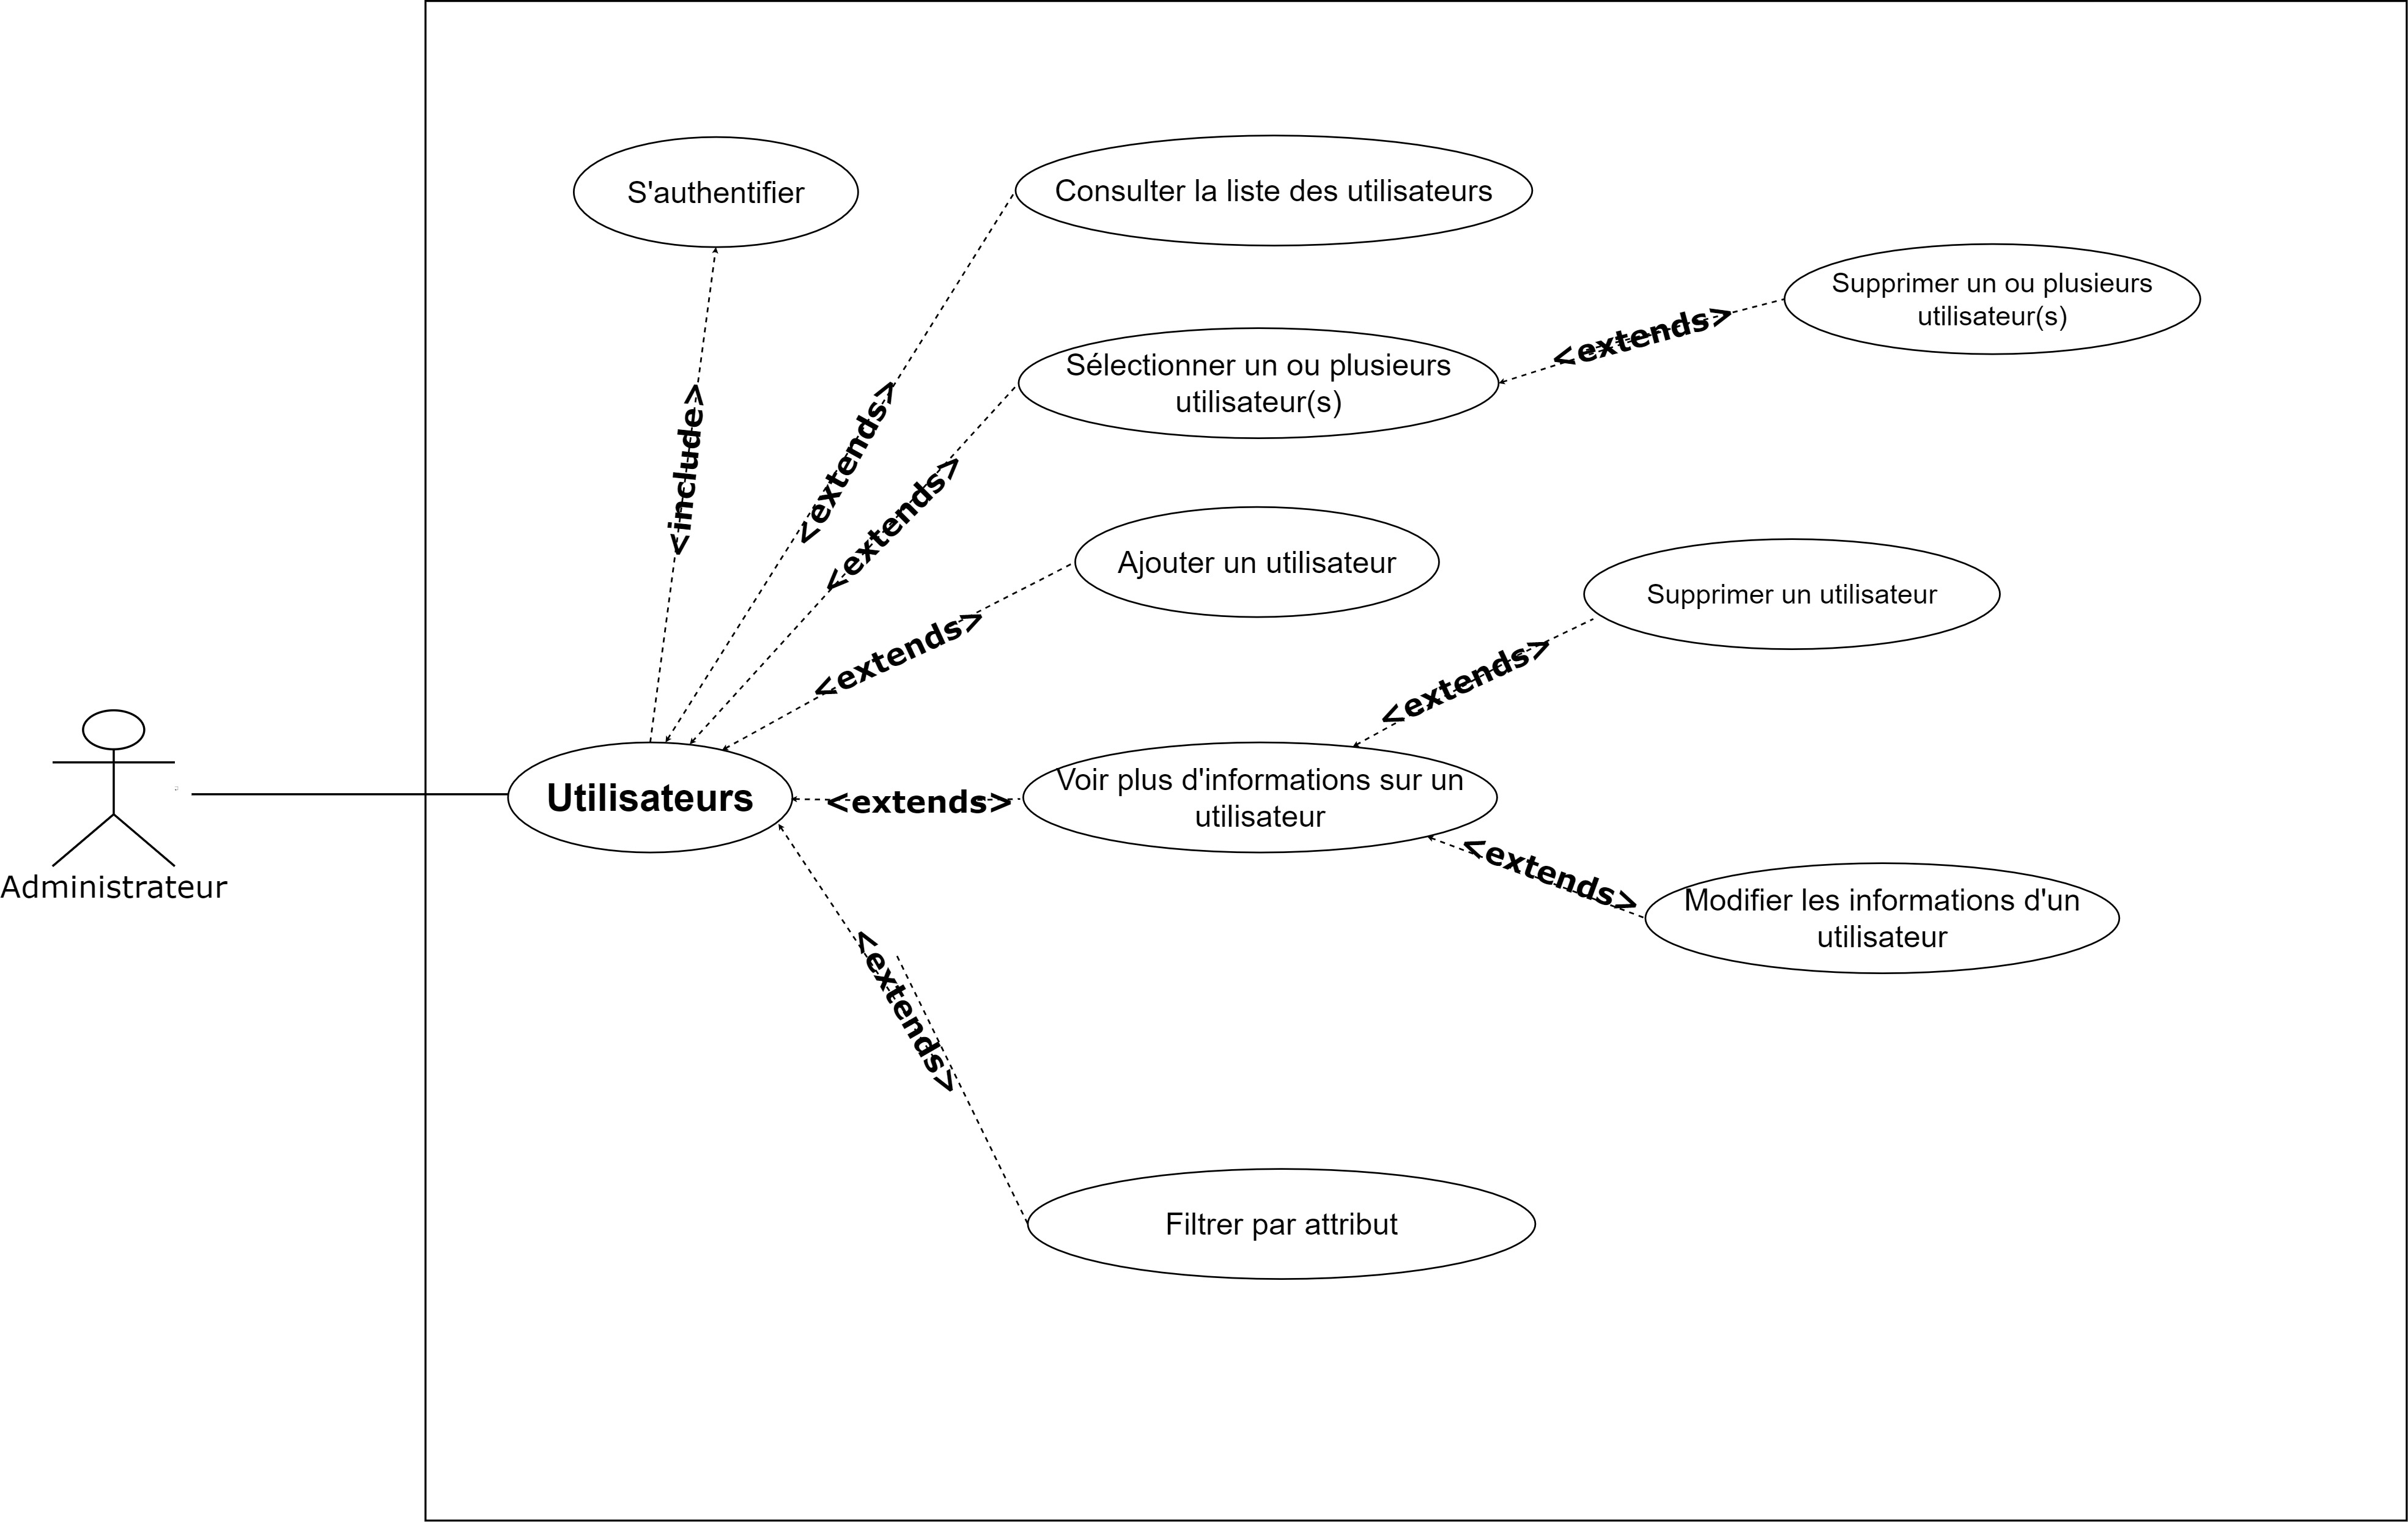
\includegraphics[scale=0.1]{ACR/Diagrammes/Utilisateurs.jpg}
    \caption{Cas d'utilisation 'Utilisateurs'}
\end{figure}


\section{Conception}
Après avoir terminé la modélisation de notre application avec différents diagrammes, nous allons passer à la phase de conception.\\

Nous commencerons par quelles ques diagrammes de séquence, puis passerons aux diagrammes de classes. Nous finirons avec une présentation de la structure globale de la base de données.\\

\subsubsection{Les diagrammes de séquence}
Les diagrammes de séquence permettent de décrire les scénarios de chaque cas d'utilisation avec une chronologie des opérations.

\paragraph*{Remarque} En vue du nombre important des cas d'utilisation de notre application, nous n'allons présenter que quelques diagrammes de séquences.\\

\subsubsection{Le diagramme de classe}
Dans la programmation orientée objet, le diagramme de classes est le plus important. Il est le seul obligatoire dans une telle modélisation\\

Le diagramme de classes a pour but de montrer la structure interne du système. Il nous permet d'avoir une vue statique et abstraite de l'ensemble des interactions des objets du système.\\

\paragraph*{Remarque} Pour le pas encombré notre diagramme de classes nous allons définir nos classes, leurs attributs et leurs méthodes d'abord. Par la suite nous définirons les associations et les relations entre les classes.\\

\begin{table}[H]
    \begin{center}
        \begin{tabular}{|Z{5cm}|}
            \hline
            \textbf{Menus}\\
            \hline
            \begin{itemize}
                \item id\_menu
                \item id\_plat\_un
                \item id\_plat\_deux
                \item id\_dessert\_un
                \item id\_dessert\_deux
                \item start
                \item end
                \item recurring
                \item until
                \item interval
                \item freq
                \item title
                \item id\_restaurant
            \end{itemize}\\
            \hline
            \begin{itemize}
                \item[+] Consulter la liste des menus()
                \item[+] Ajouter un menu()
                \item[+] Modifier un menu()
                \item[+] Supprimer un menu()
            \end{itemize}
            \\
            \hline
        \end{tabular}	
        \caption{Classe Menus}
    \end{center}
\end{table}

\begin{table}[H]
    \begin{center}
        \begin{tabular}{|Z{5cm}|}
            \hline
            \textbf{Dossiers de bourse}\\
            \hline
            \begin{itemize}
                \item id\_dossier\_b
                \item nom
                \item prenom
                \item n\_etudiant
                \item n\_tel
                \item email
                \item photo\_id
                \item demande\_b\_sign
                \item attestation\_bac
                \item cert\_scolarite
                \item ext\_naissance
                \item accepted
                \item date\_depot
                \item ext\_role\_impo\_pere
                \item ext\_role\_impo\_mere
                \item ext\_role\_impo\_etud
                \item just\_rev\_pere
                \item just\_rev\_mere
                \item spec\_cheq
            \end{itemize}\\
            \hline
            \begin{itemize}
                \item[+] Consulter la liste des dossiers de bourse()
                \item[+] Consulter les détails d'un seul dossier de bourse()
                \item[+] Ajouter un dossiers de bourse()
                \item[+] Valider un dossiers de bourse()
                \item[+] Refuser un dossiers de bourse()
            \end{itemize}
            \\
            \hline
        \end{tabular}	
        \caption{Classe Dossiers de bourse}
    \end{center}
\end{table}

\begin{table}[H]
    \begin{center}
        \begin{tabular}{|Z{5cm}|}
            \hline
            \textbf{Utilisateurs}\\
            \hline
            \begin{itemize}
                \item id\_user
                \item email
                \item password
                \item displayName
                \item role
            \end{itemize}\\
            \hline
            \begin{itemize}
                \item[+] Consulter la liste des utilisateurs()
                \item[+] Consulter les détails d'un seul utilisateur() 
                \item[+] Ajouter un utilisateur()
                \item[+] modifier un utilisateur()
                \item[+] supprimer un utilisateur()
            \end{itemize}
            \\
            \hline
        \end{tabular}	
        \caption{Classe Utilisateurs}
    \end{center}
\end{table}

\begin{table}[H]
    \begin{center}
        \begin{tabular}{|Z{5cm}|}
            \hline
            \textbf{Trajets}\\
            \hline
            \begin{itemize}
                \item id\_trajet
                \item id\_bus
                \item start
                \item end
                \item recurring
                \item until
                \item interval
                \item freq
                \item title
            \end{itemize}\\
            \hline
            \begin{itemize}
                \item[+] Consulter la liste des trajets()
                \item[+] Consulter les détails d'un seul trajet() 
                \item[+] Ajouter un trajet()
                \item[+] modifier un trajet()
                \item[+] supprimer un trajet()
            \end{itemize}
            \\
            \hline
        \end{tabular}	
        \caption{Classe Trajets}
    \end{center}
\end{table}

\begin{table}[H]
    \begin{center}
        \begin{tabular}{|Z{5cm}|}
            \hline
            \textbf{Bus}\\
            \hline
            \begin{itemize}
                \item id\_bus
                \item matricule
                \item adr\_depart
                \item adr\_arrivee
                \item actif
            \end{itemize}\\
            \hline
            \begin{itemize}
                \item[+] Consulter la liste des bus()
                \item[+] Ajouter un bus()
                \item[+] modifier un bus()
                \item[+] supprimer un bus()
            \end{itemize}
            \\
            \hline
        \end{tabular}	
        \caption{Classe Bus}
    \end{center}
\end{table}

\begin{table}[H]
    \begin{center}
        \begin{tabular}{|Z{5cm}|}
            \hline
            \textbf{Campus et Résidence}\\
            \hline
            \begin{itemize}
                \item id\_camp\_res
                \item nom
                \item adresse
                \item nbr\_lits
            \end{itemize}\\
            \hline
            \begin{itemize}
                \item[+] Consulter la liste des campus et des résidences()
                \item[+] Ajouter un campus ou une résidence()
                \item[+] modifier un campus ou une résidence()
                \item[+] supprimer un campus ou une résidence()
            \end{itemize}
            \\
            \hline
        \end{tabular}	
        \caption{Classe Campus et Résidence}
    \end{center}
\end{table}

\begin{table}[H]
    \begin{center}
        \begin{tabular}{|Z{5cm}|}
            \hline
            \textbf{Dossiers d'Hébergement}\\
            \hline
            \begin{itemize}
                \item id\_dossier
                \item nom
                \item prenom
                \item n\_etudiant
                \item n\_tel
                \item email
                \item photo\_id
                \item demande\_sign
                \item attestation\_bac
                \item cert\_scolarite
                \item cert\_residence
                \item ext\_naissance
                \item accepted
                \item archived
                \item date\_depot
                \item selected\_res
            \end{itemize}\\
            \hline
            \begin{itemize}
                \item[+] Consulter la liste des dossiers d'hébergement()
                \item[+] Ajouter un dossier d'hébergement()
                \item[+] Valider un dossier d'hébergement()
                \item[+] Refuser un dossier d'hébergement()
            \end{itemize}
            \\
            \hline
        \end{tabular}	
        \caption{Classe Dossiers d'Hébergement}
    \end{center}
\end{table}

\begin{table}[H]
    \begin{center}
        \begin{tabular}{|Z{5cm}|}
            \hline
            \textbf{Réstaurants}\\
            \hline
            \begin{itemize}
                \item id\_restaurant
                \item id\_camp\_res
                \item nom
            \end{itemize}\\
            \hline
            \begin{itemize}
                \item[+] Consulter la liste des réstaurants()
                \item[+] Ajouter un réstaurant()
                \item[+] Modifier un réstaurant()
                \item[+] Supprimer un réstaurant()
            \end{itemize}
            \\
            \hline
        \end{tabular}	
        \caption{Classe Réstaurants}
    \end{center}
\end{table}

\begin{table}[H]
    \begin{center}
        \begin{tabular}{|Z{5cm}|}
            \hline
            \textbf{Desserts}\\
            \hline
            \begin{itemize}
                \item id\_dessert
                \item nom
                \item prix
                \item qte\_stock
                \item description
            \end{itemize}\\
            \hline
            \begin{itemize}
                \item[+] Consulter la liste des desserts()
                \item[+] Ajouter un dessert()
                \item[+] Modifier un dessert()
                \item[+] Supprimer un dessert()
            \end{itemize}
            \\
            \hline
        \end{tabular}	
        \caption{Classe Desserts}
    \end{center}
\end{table}

\begin{table}[H]
    \begin{center}
        \begin{tabular}{|Z{5cm}|}
            \hline
            \textbf{Plats}\\
            \hline
            \begin{itemize}
                \item id\_plat
                \item nom
                \item description
            \end{itemize}\\
            \hline
            \begin{itemize}
                \item[+] Consulter la liste des plats()
                \item[+] Ajouter un plat()
                \item[+] Modifier un plat()
                \item[+] Supprimer un plat()
            \end{itemize}
            \\
            \hline
        \end{tabular}	
        \caption{Classe Plats}
    \end{center}
\end{table}

\begin{table}[H]
    \begin{center}
        \begin{tabular}{|Z{5cm}|}
            \hline
            \textbf{Contient}\\
            \hline
            \begin{itemize}
                \item quantite
            \end{itemize}\\
            \hline
        \end{tabular}	
        \caption{Classe Ingrédients d'un Plat}
    \end{center}
\end{table}

\begin{table}[H]
    \begin{center}
        \begin{tabular}{|Z{5cm}|}
            \hline
            \textbf{Ingrédients}\\
            \hline
            \begin{itemize}
                \item id\_ingredient
                \item nom
                \item prix
                \item qte\_stock
            \end{itemize}\\
            \hline
            \begin{itemize}
                \item[+] Consulter la liste des ingrédients()
                \item[+] Ajouter un ingredient()
                \item[+] Modifier un ingredient()
                \item[+] Supprimer un ingredient()
            \end{itemize}
            \\
            \hline
        \end{tabular}	
        \caption{Classe Ingrédients}
    \end{center}
\end{table}


\begin{figure}[H]
    \centering
    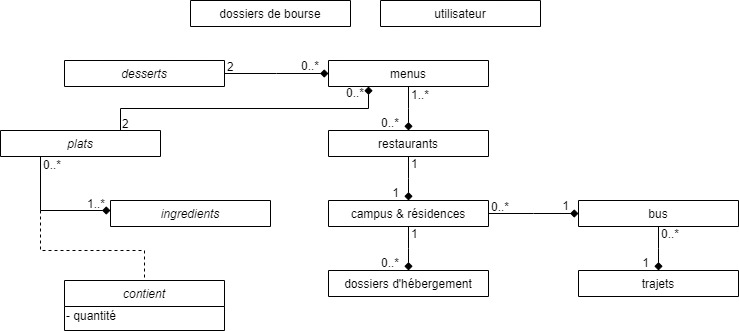
\includegraphics[scale=0.55]{ACR/Diagrammes/class.jpg}
    \caption{Diagramme de classe}
\end{figure}

\subsubsection{Structure de la base de données}
\begin{figure}[H]
    \centering
    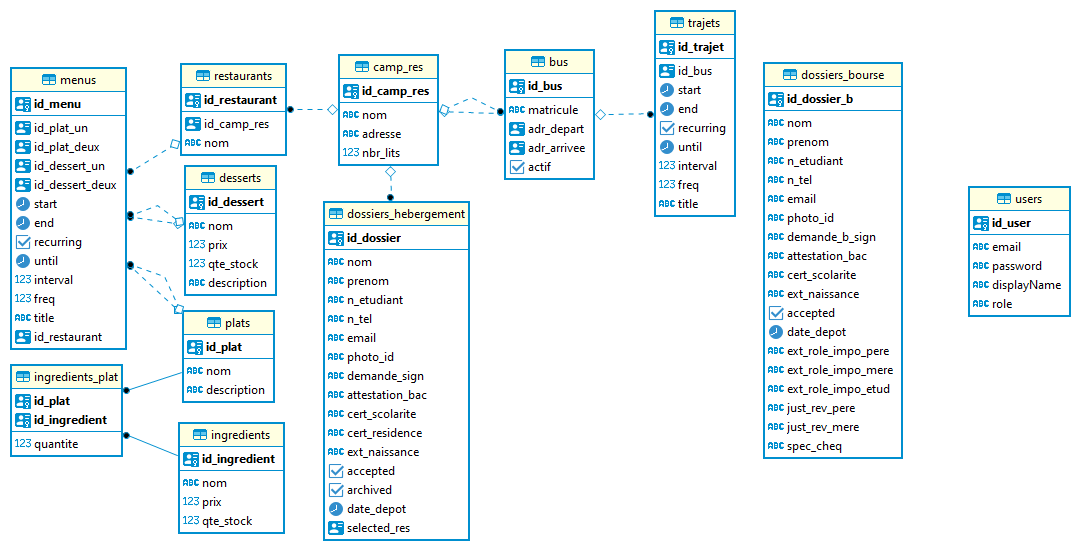
\includegraphics[scale=0.38]{ACR/Diagrammes/diag.png}
    \caption{Structure de la base de données}
\end{figure}

\section{Conclusion}
À l'aide de l'analyse et de la conception, nous avons établi une description graphique de notre projet à travers une utilisation d'\acs{UML} et de ses diagrammes.\\

Nous avons commencé par une présentation et une définition d'\acs{UML} et de ses différents diagrammes.\\

Par la suite, dans la partie analysée, nous avons spécifié les besoins fonctionnels et non fonctionnels de notre application. Ceci nous a mené à l'identification des différents acteurs qui interagissent avec notre système et la spécification des taches de chacun d'eux, ainsi qu'une représentation dès les multiples cas d'utilisation de notre application\\

Finalement, nous sommes passé à la partie conception, où nous avons présenté les différents scénarios du système à l'aide des diagrammes de séquence. Nous avons aussi présenté la structure interne du système à l'aide des diagrammes de classes ainsi qu'une présentation globale de la structure de la base de données.\\

Après avoir analysé et conceptualiser notre système nous allons passer à la partie suite qui est la réalisation de l'application.
		% \chapter{Réalisation}

\section{Introduction}
    Dans ce chapitre nous allons présenter l'environnement de développement de l'application.\\

    Nous commencerons par les techniques utilisés puis passerons vers les bibliothèques et les frameworks qui ont aidé dans cette réalisation. Par la suite, nous présenterons les outils utilisés tout le long du processus de création.\\

    Finalement, nous présenterons quelles ques interfaces de l'application.\\

\section{Présentation des technologies utilisées}
    Le but du projet est la création d'une application full-stack web. pour cela, plusieurs outils peuvent être utilisés, parmi ces outils, nous avons choisi \acs{PERN} qui est une pile de technologies conçues justement pour la création d'un environnement de développement full-stack web. \acs{PERN}, par ses initiales, se compose de PostgreSQL, ExpressJS, React et Node.js.\\

    \acs{PERN} est un substitué de \acs{MERN}, qui est lui-même composer de MongoDB, ExpressJS, React et Node.js. Comme \acs{MERN}, \acs{PERN} donne la possibilité de créer des applications web full-stack avec des opérations \acs{CRUD} (Create, Read, Update, Delete). Mais \acs{PERN} utilise PostgreSQL au lieu de MongoDB est nous offre un grand support pour les fonctionnalités \acs{NoSQL}, avec une forte conformité aux normes et prend en compte les transactions.\\

    \subsection{PostgreSQL}
    \begin{figure}[H]
        \centering
        
\includegraphics[scale=0.2]{ACR/postgresql.png}
        \caption{Logo PostgreSQL}
    \end{figure}
    
    PostgreSQL\cite{postgres} est système de gestion de base de données relationnel orienté objet puissant et open-source, qui utilise \acs{SQL} et prend en charge en toute sécurité les charges de travil complexes en regroupant plusieurs fonctionnalités qui donnent priorité à l'extensibilité et la conformité.\\

    L'origine de PostgreSQL remonte a la base de données Ingres développer à l'université de la Californie de Berkley par Michael Stonebraker. Au années 1986, son créateur a repris le projet de zero est a décidé de le nommée POSTGRES, comme pour dire post-ingres. Ce n'est qu'en 1995 que son créateur à décidé d'ajouter les fonctionnalitées \acs{SQL} est a été renommée Postgre95, et ce fut qu'à la fin des années 1996 qu'il a été renommée en PostgreSQL.\\
    
    Avec plus de 30 années de développement, PostgreSQL a gagné une forte réputation grace a son architecture, sa robustesse, son extensibilité et le dévouement des contributeurs de la communauté open-source.\\

    \subsection{ExpressJS}
    \begin{figure}[H]
        \centering
        
\includegraphics[scale=0.16]{ACR/ExpressJS-logo.png}
        \caption{Logo ExpressJS}
    \end{figure}
    
    ExpressJS\cite{expressjs} est un framework Node.js qui fournit des fonctions puissantes pour les applications web et mobiles. Il est très simple, très léger et très flexible. Il apporte très peu de couverture et maintient le meilleur côté et une exécution rapide.\\

    En vue de son côté open source et facile d'utilisation, ExpressJS connaît une grande notoriété et possède grace aux contributeurs une grande bibliothèque de modules prêt à l'employer. ExpressJS améliore Node.js, de façons à construire rapidement, facilement et efficacement les APIs les plus complexes.\\ 

    \subsection{React}
    \begin{figure}[H]
        \centering
        
\includegraphics[scale=0.16]{ACR/react.png}
        \caption{Logo REACT}
    \end{figure}

    React\cite{react} est une bibliothèque JavaScript conçue pour créer des interfaces utilisateur interactives et rapides pour les applications Web et mobiles. React a été créé par Jordan Walke, ingénieur logiciel chez Facebook.\\
    
    React s'agit d'une bibliothèque frontend open source, basée sur des composants réutilisables, qui n'est responsable que de la couche de vue (View) des application basé sur l'architecture Model View Controller (\acs{MVC}). L'une des forces de React est la modification de données sans rechargement de page. Cette spécialisation permet à React d'être combiné avec plusieurs bibliothèques ou frameworks pour former une application fullstack.\\

    \subsection{Node.js}
    \begin{figure}[H]
        \centering
        
\includegraphics[scale=0.1]{ACR/nodejs-logo.png}
        \caption{Logo Node.js}
    \end{figure}

    Node.js\cite{nodejs} est un environnement d'exécution JavaScript open source et multiplateforme qui peut exécuter du code JavaScript en dehors du navigateur Web. Node.js est un framework Web léger et populaire, adapté aux débutants, mais aussi utilisé dans de nombreuses grandes entreprises telles que Netflix et Uber l'utilisent.\\
    
    Node.js est un framework Web très approprié pour les débutants, il permet de pouvoir facilement démarrer la construction back-end. Il nous permet d'utiliser JavaScript n'importe où et sur n'importe quel navigateur, y compris MacOS, Linux et Windows. Quand nous disons omniprésent, nous faisons référence au front-end, au middleware et au back-end. Par conséquent, Node.js fait partie de certaines piles de développement Web très populaires, telles que la pile \acs{MERN}, la pile \acs{MEVN} et la pile \acs{MEAN}.\\

\section{Bibliothèques et Framework utilisés}
    Le but des bibliothèques et des frameworks est de nous faciliter et d'acculer le processus de développement. Celle-ci nous apportent des fonctions déjà créées et ne nous restent plus qu'a les utilisé.\\

    Voici donc qu'elles unes de ces bibliothèques et frameworks:\\

    \subsection{Axios}
    \begin{figure}[H]
        \centering
        
\includegraphics[scale=1]{ACR/axios-logo.png}
        \caption{Logo Axios}
    \end{figure}

    Axios\cite{axios} est un client HTTP basé sur des promesses qui peut s'exécuter dans un navigateur et un environnement Node.js. Il fournit une API pour traiter les requêtes XMLHttpRequests et l'interface http du nœud. De plus, il utilise également la requête d'emballage polyfill de la nouvelle syntaxe de promesse d'ES6.\\
    
    Presque tous les projets dynamiques que vous créez doivent interagir avec l'API RESTFUL à un moment donné, et l'utilisation d'Axios est un moyen simple de le faire. La première version d'Axios est sortie il y a environ 4 ans, et son code open source est disponible sur GitHub. Axios compte plusieurs contributeurs qui ont contribué à chaque version d'Axios.\\

    \subsection{Redux}
    \begin{figure}[H]
        \centering
        
\includegraphics[scale=0.2]{ACR/redux-logo.png}
        \caption{Logo Redux}
    \end{figure}

    Redux\cite{redux} est une bibliothèque JavaScript open source pour la gestion des "state" de l'application. Redux est généralement utilisé avec des bibliothèques telles que Angular ou React pour créer des interfaces utilisateur. Il a été créé par Andrew Clark et Dan Abramov.\\
    
    Lorsque la taille de l'application devient très importante, il devient difficile de gérer le state de chaque composant de l'application. Il permet de mettre à jour et de maintenir le state de chaque composant de l'application.\\

    React ne traite pas la gestion des objets du state, garantissant que l'un des moyens pour résoudre ce problème est via Redux. Les données d'application de React circulent du composant parent vers le composant enfant. Les données du composant parent peuvent être envoyées au composant enfant sous la forme d'accessoires. Il y a trop de composants dans React et il est difficile de suivre le flux de données du composant parent au composant enfant. Par conséquent, nous utilisons Redux en raison de sa capacité à gérer tout le state du composant.\\

    \subsection{JWT}
    \begin{figure}[H]
        \centering
        
\includegraphics[scale=0.4]{ACR/jwt-logo.png}
        \caption{Logo JWT}
    \end{figure}

    JSON Web Token\cite{jwt} (\acs{JWT}) est une norme ouverte (RFC 7519) qui définit une méthode compacte et autonome pour la transmission sécurisée d'informations entre les parties (telles qu'un client et un serveur) en tant qu'objets JSON. Étant donné que ces informations sont signées numériquement, elles peuvent être vérifiées et fiables. \acs{JWT} peut être signé à l'aide d'un secret (à l'aide de l'algorithme HMAC) ou à l'aide d'une paire de clés publique/privée RSA ou ECDSA.\\
    
    \acs{JWT} est particulièrement populaire dans le processus d'authentification. Leurs messages courts peuvent être cryptés et peuvent indiquer en toute sécurité qui est l'expéditeur et s'il dispose des droits d'accès nécessaires. L'utilisateur lui-même n'a pas de contact indirect avec le token, par exemple lorsqu'il saisit le nom d'utilisateur et le mot de passe dans le masque. La vraie communication a lieu entre le client et le serveur.\\

    \subsection{Material UI}
    \begin{figure}[H]
        \centering
        
\includegraphics[scale=0.4]{ACR/materialui-logo.png}
        \caption{Logo Material UI}
    \end{figure}

    Material UI\cite{mui} est l'un des frameworks d'interface utilisateur React des plus reconnu. Il nous fournit des composants React qui implémentent Google Material Design. Material-UI a commencé avec l'implémentation React de la spécification Google Material Design en 2014.\\

    Material UI contiens plusieurs composants prêt a l'emploi et donne, donc, aux développeurs une très grande rapidité lors de la création des interfaces. Il est aussi très facile à personnaliser ce qui fait de lui l'un des frameworks les plus utilisés quand il s de création d'interfaces utiliser.\\

\section{Présentation des outils utilisés}
    \subsection{Visual Studio Code}
    \begin{figure}[H]
        \centering
        
\includegraphics[scale=0.1]{ACR/vscode-logo.png}
        \caption{Logo Visual Studio Code}
    \end{figure}

    Visual Studio Code\cite{vscode} est un éditeur de code source qui peut être utilisé dans plusieurs langages de programmation. Il est basé sur le framework Electron et est utilisé pour développer des applications Web Node.js s'exécutant sur le moteur de mise en page Blink.\\
    
    Visual Studio Code peut être étendu via des extensions, ce qui le rend très versatile, qui sont disponibles via un dépôt central. Cela inclut l'ajout d'un éditeur et la prise en charge des langues. Une caractéristique notable est la possibilité de créer des extensions pour ajouter la prise en charge de nouveaux langages, thèmes et débogueurs, d'effectuer une analyse de code statique.\\
    
    Dans l'enquête auprès des développeurs Stack Overflow de 2021, Visual Studio Code a été classé comme l'outil d'environnement de développement le plus populaire.

    \subsection{Dbeaver}
    \begin{figure}[H]
        \centering
        
\includegraphics[scale=0.1]{ACR/DBeaver-Logo.png}
        \caption{Logo DBeaver}
    \end{figure}
    
    DBeaver\cite{dbeaver} est un outil de gestion de base de données graphique gratuit et open source pour les développeurs et les administrateurs de base de données. Prêt à l'emploi, DBeaver prend en charge plus de 80 bases de données.\\
    
    À l'aide de DBeaver, on a la possibilité de manipuler les données comme dans des feuilles de calcul ordinaires, créer des rapports d'analyse basés sur les enregistrements de différents magasins de données et exporter des informations dans un format approprié. Pour les utilisateurs avancés de bases de données, DBeaver recommande l'utilisation d'un éditeur SQL puissant, de fonctions de gestion étendues, de fonctions de migration de données et de schémas, de surveillance des sessions de connexion à la base de données, etc.\\
    
    DBeaver est un outil multiplateforme disponible pour Windows, Linux, Mac et Solaris.\\

    \subsection{Github}
    \begin{figure}[H]
        \centering
        \includegraphics[scale=0.4]{ACR/Github-Logo.png}
        \caption{Logo Github}
    \end{figure}

    GitHub\cite{github} est une plate-forme de gestion de versions et de collaboration open source pour les développeurs de logiciels. La solution GitHub livrée sous forme de logiciel à la demande (SaaS, Software as a Service) a été lancée en 2008.\\
    
    Il est basé sur Git, un système de gestion de code open source créé par Linus Torvalds pour accélérer le développement de logiciels. L'interface de GitHub est très conviviale, même les codeurs novices peuvent profiter de Git. Si vous n'avez pas GitHub, l'utilisation de Git nécessite généralement plus de connaissances techniques et d'utilisation de la ligne de commande.\\

    \subsection{Discord}
    \begin{figure}[H]
        \centering
        
\includegraphics[scale=0.09]{ACR/Discord-Logo.png}
        \caption{Logo Discord}
    \end{figure}
    
    Discord\cite{discord} est une plate-forme de chat et de messagerie en ligne conçue pour une utilisation en groupe. Comme il est réservé aux invités, il s'agit d'un espace sûr où les étudiants peuvent interagir sans avoir à rester ensemble dans la pièce. L'application de messagerie d'équipe se concentre principalement sur le chat vocal. L'option de chat textuel n'est pas aussi étendue que le canal vocal dans ses produits.\\

    Il s'agit d'un système très facile à utiliser et qui peut également être mis en place rapidement. Par conséquent, cela peut faciliter la transition vers l'enseignement à distance ou les classes hybrides, tout en créant l'impression que tout le monde est dans la même pièce. La vidéo et l'audio à faible latence permettent d'obtenir une réponse quasi instantanée, tout comme le chat dans le monde réel.\\

    \subsection{Draw.io}
    \begin{figure}[H]
        \centering
        
\includegraphics[scale=0.4]{ACR/Drawio-Logo.png}
        \caption{Logo Draw.io}
    \end{figure}

    Draw.io\cite{drawio} est conçu par Seibert Media et est un logiciel propriétaire permettant de créer des tableaux et des graphiques. Le logiciel vous permet de sélectionner des fonctions de mise en page automatiques ou de créer des mises en page personnalisées. Ils ont une variété de formes et des centaines d'éléments visuels parmi lesquels choisir, ce qui rend votre tableau ou graphique unique. La fonction glisser-déposer peut facilement créer des tableaux ou des graphiques attrayants.\\

    Par rapport à l'utilisation d'un logiciel vectoriel, cet outil peut vous aider à créer plus facilement des diagrammes et d'autres effets visuels. Lorsqu'il est utilisé avec Google Drive, Draw.io prend en charge la collaboration en temps réel afin que plusieurs personnes puissent travailler sur le graphique en même temps.\\

\section{Présentation des interfaces}
    Dans le contenu suivant, nous montrerons un aperçu du rendu final de notre application et quelle ques interfaces qui la composent.

    \subsection{Interface d'accueil}
    \begin{figure}[H]
        \centering
        
\includegraphics[scale=0.21]{PFE Screens/Invité/accueil.jpg}
        \caption{Interface d'accueil}
    \end{figure}

    \subsection{Interface d'authentification}
    \begin{figure}[H]
        \centering
        
\includegraphics[scale=0.21]{PFE Screens/Connection.jpg}
        \caption{Interface d'authentification}
    \end{figure}

    \subsection{Interface invité 'Services'}
    \begin{figure}[H]
        \centering
        \includegraphics[scale=0.21]{PFE Screens/Invité/Services.jpg}
        \caption{Interface invité 'Services'}
    \end{figure}

    \subsection{Interface invité 'Calendrier des menus'}
    \begin{figure}[H]
        \centering
        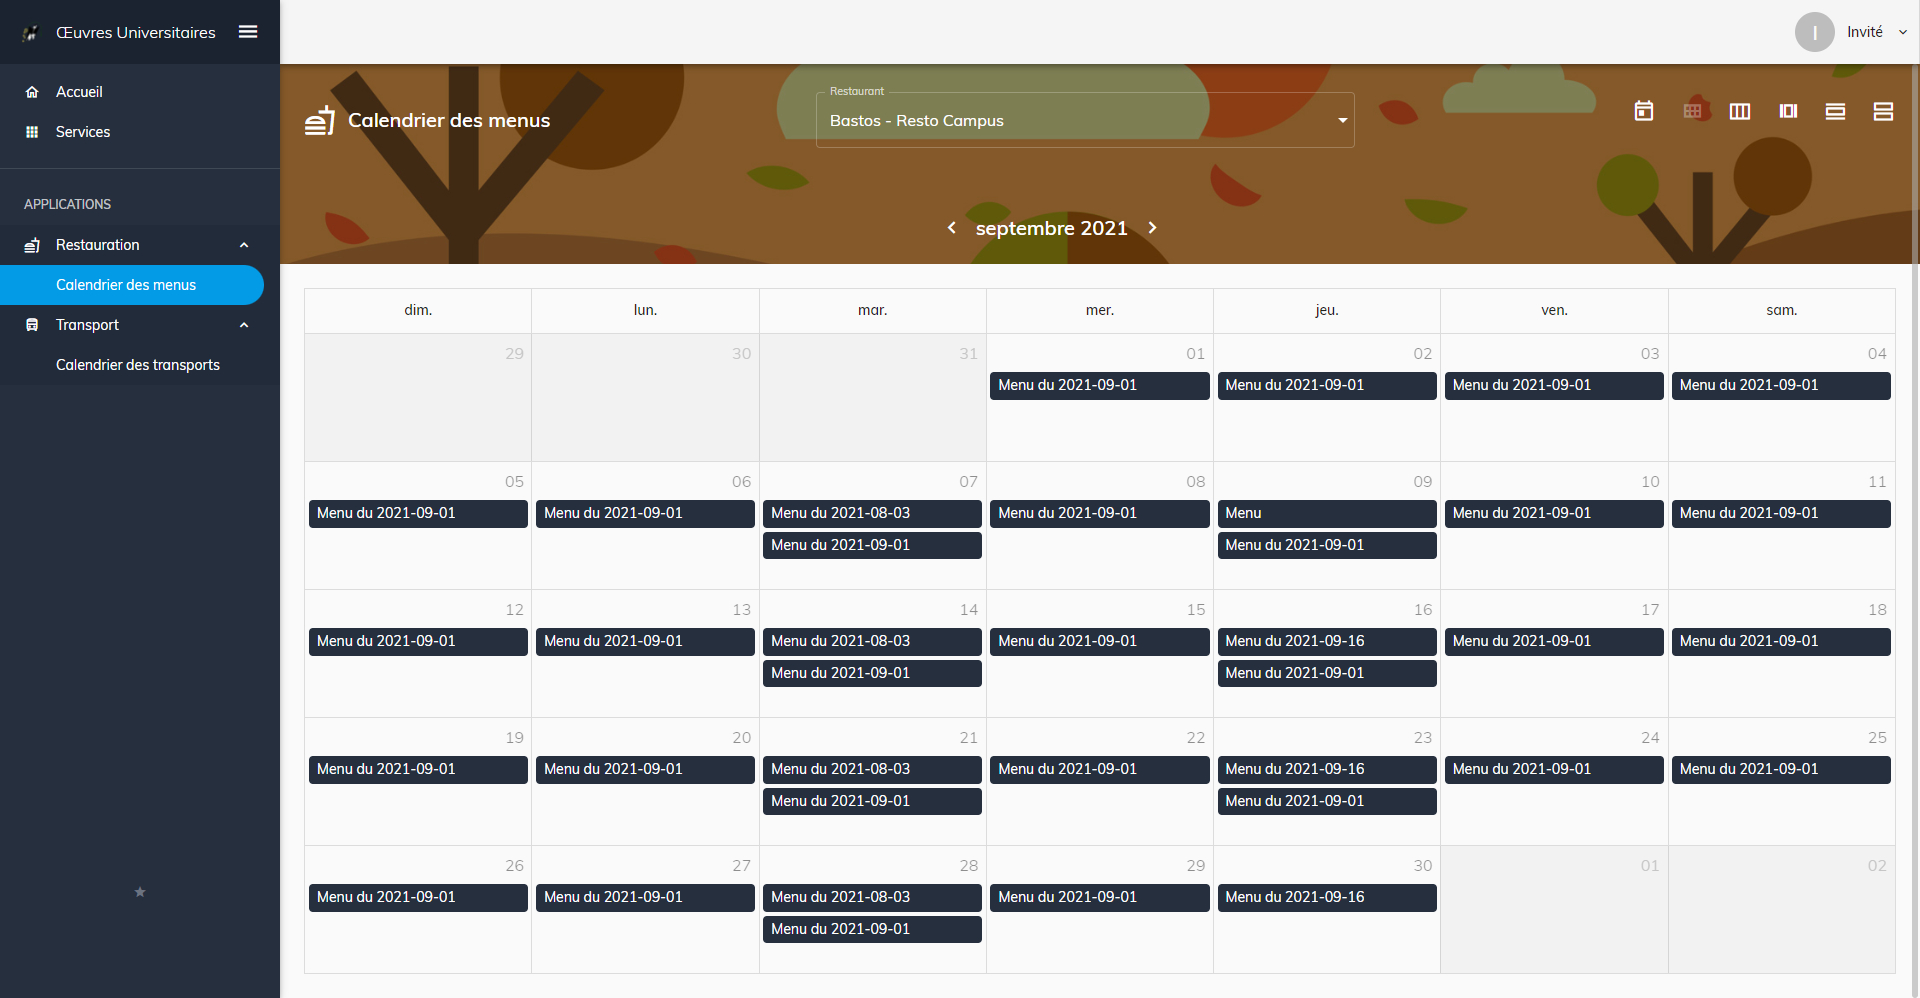
\includegraphics[scale=0.21]{PFE Screens/Invité/Restauration/Calendrier des menus.jpg}
        \caption{Interface invité 'Calendrier des menus'}
    \end{figure}

    \subsection{Interface invité 'Détail d'un menus'}
    \begin{figure}[H]
        \centering
        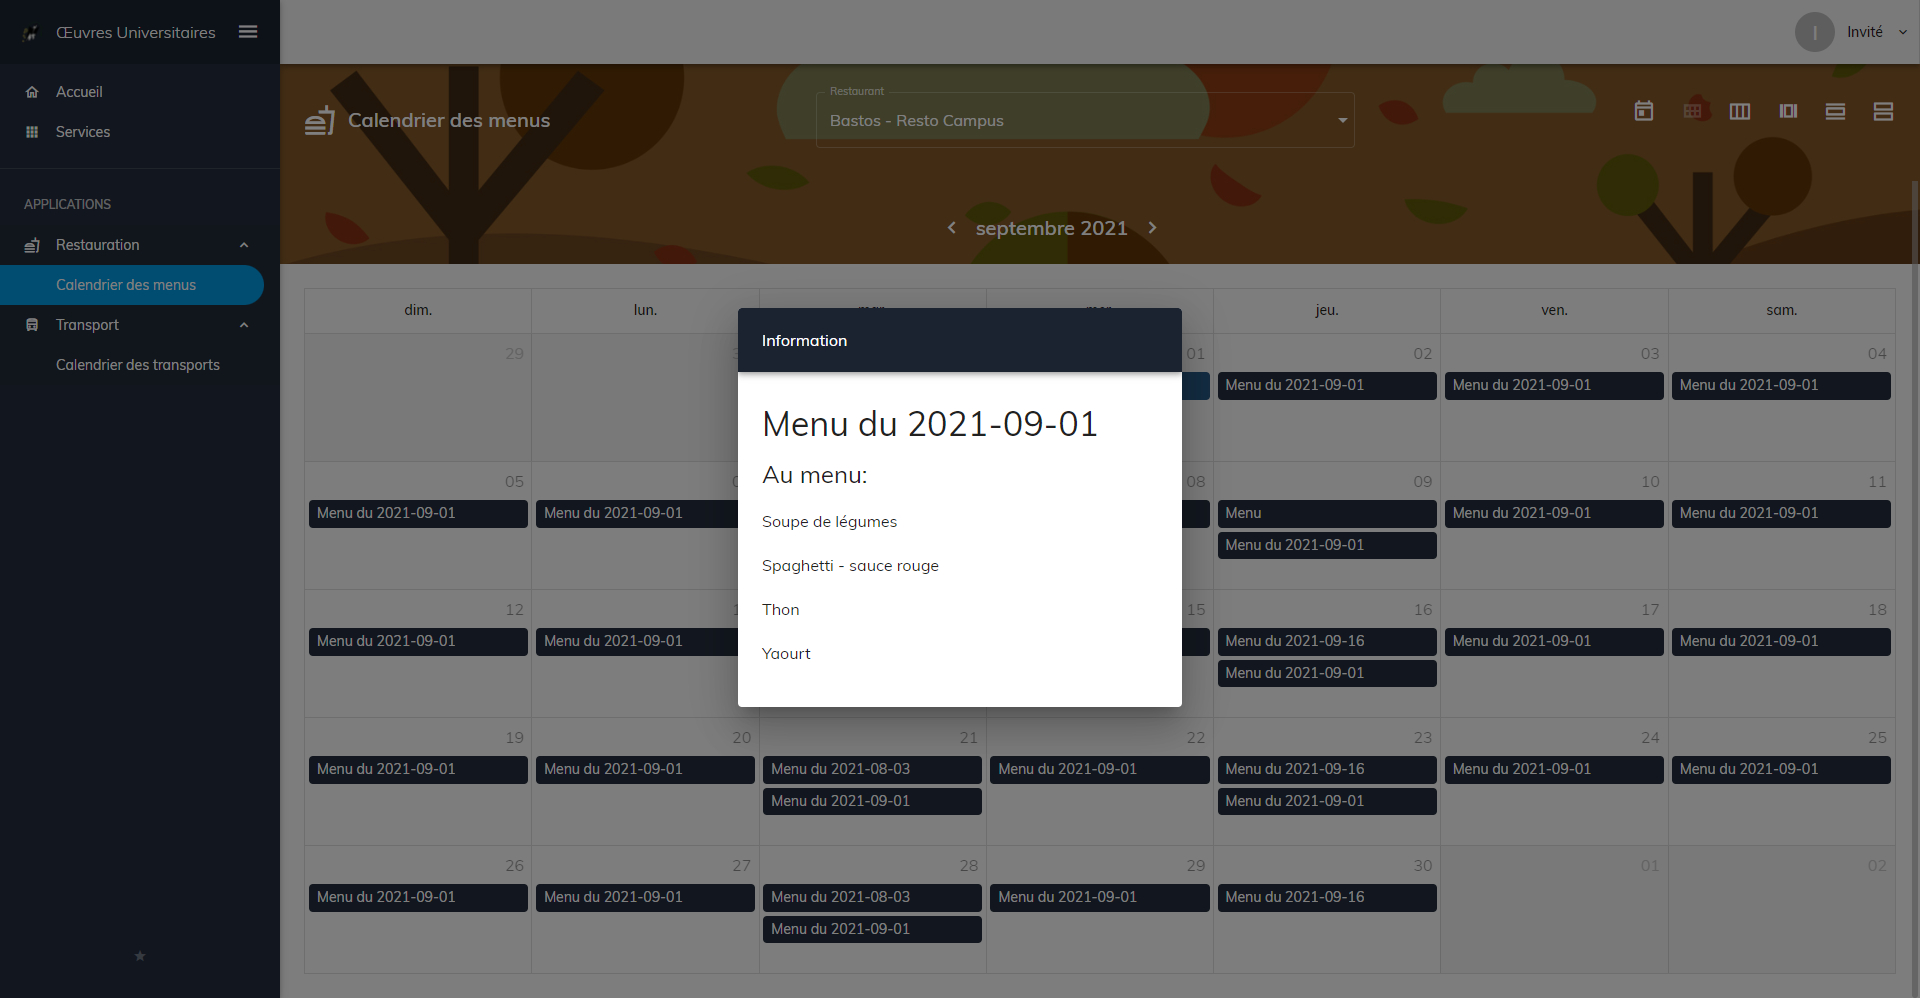
\includegraphics[scale=0.21]{PFE Screens/Invité/Restauration/Calendrier des menus - Détail.jpg}
        \caption{Interface invité 'Détail d'un menus'}
    \end{figure}
    
    \subsection{Interface d'accueil utilisateur}
    \begin{figure}[H]
        \centering
        
\includegraphics[scale=0.21]{PFE Screens/Admin/Accueil.jpg}
        \caption{Interface d'accueil utilisateur}
    \end{figure}

    \subsection{Interface utilisateur utilisateur 'Dossiers d'hebergements'}
    \begin{figure}[H]
        \centering
        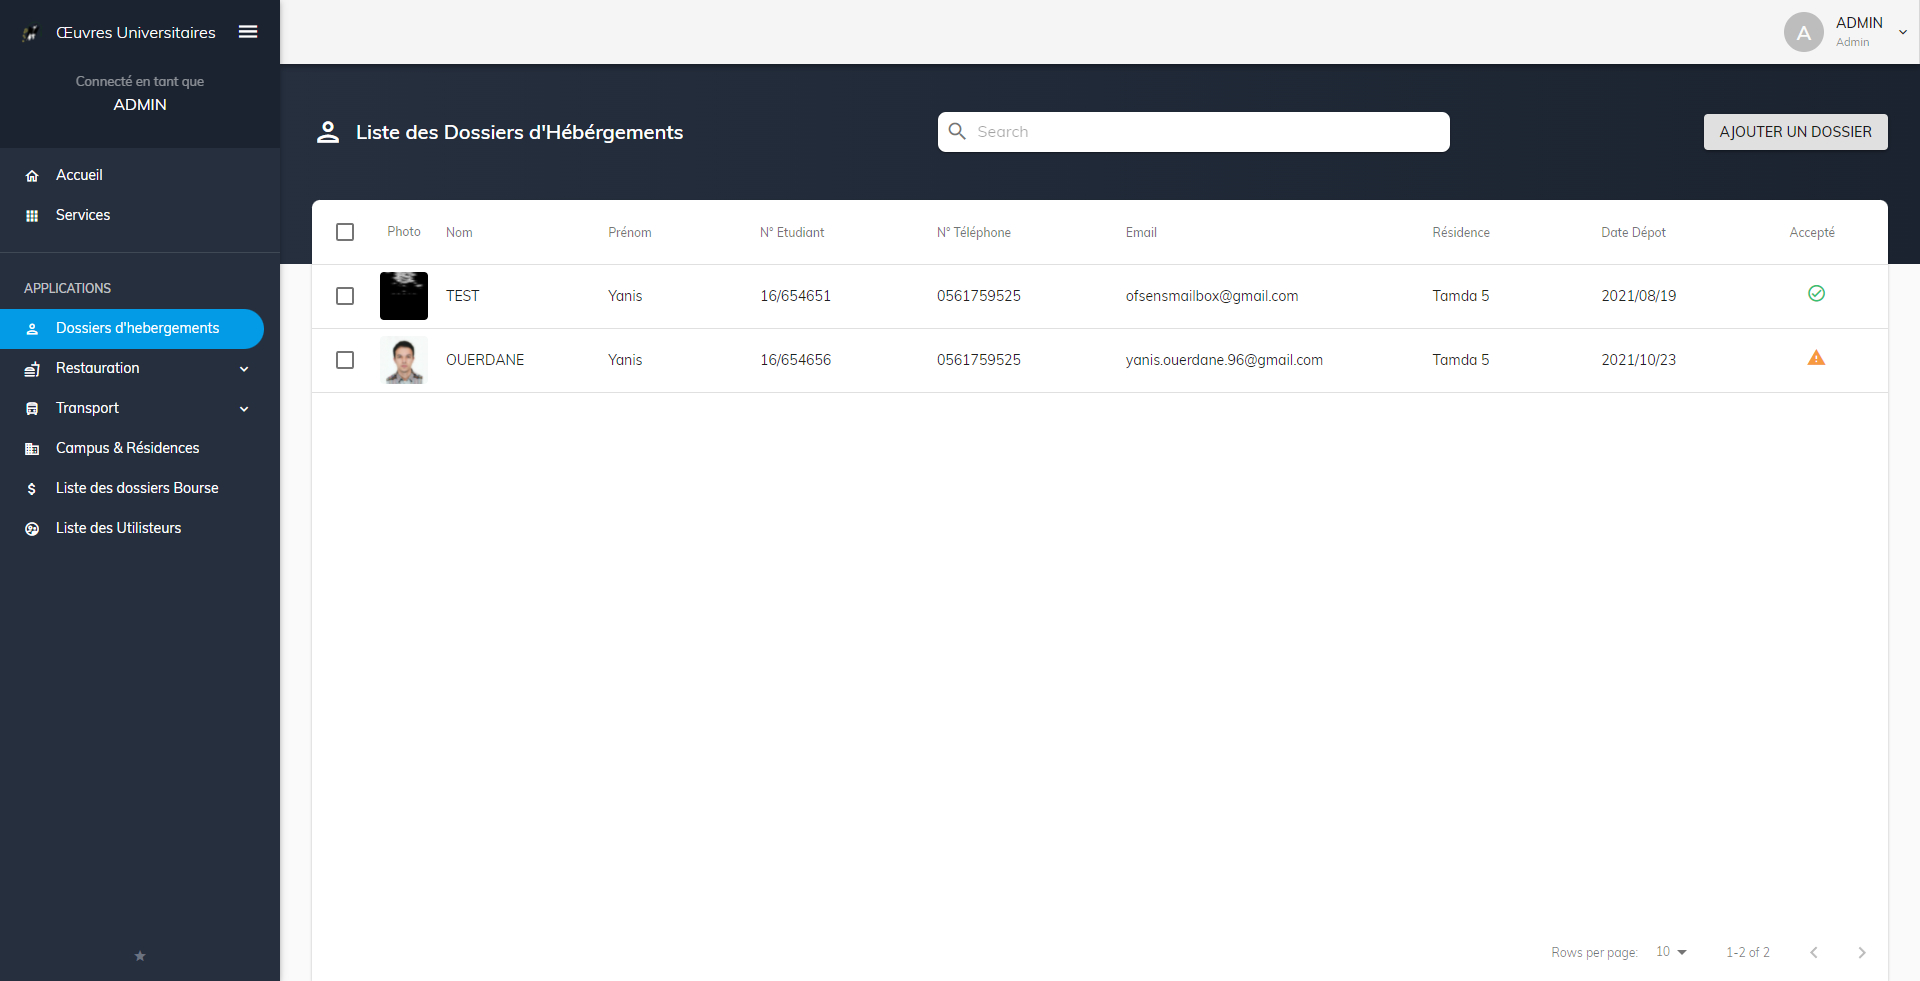
\includegraphics[scale=0.21]{PFE Screens/Admin/Hebergement/Liste des Dossiers d'Hébérgements.jpg}
        \caption{Interface utilisateur 'Dossiers d'hebergements'}
    \end{figure}

    \subsection{Interface utilisateur détail d'un dossier d'hebergements}
    \begin{figure}[H]
        \centering
        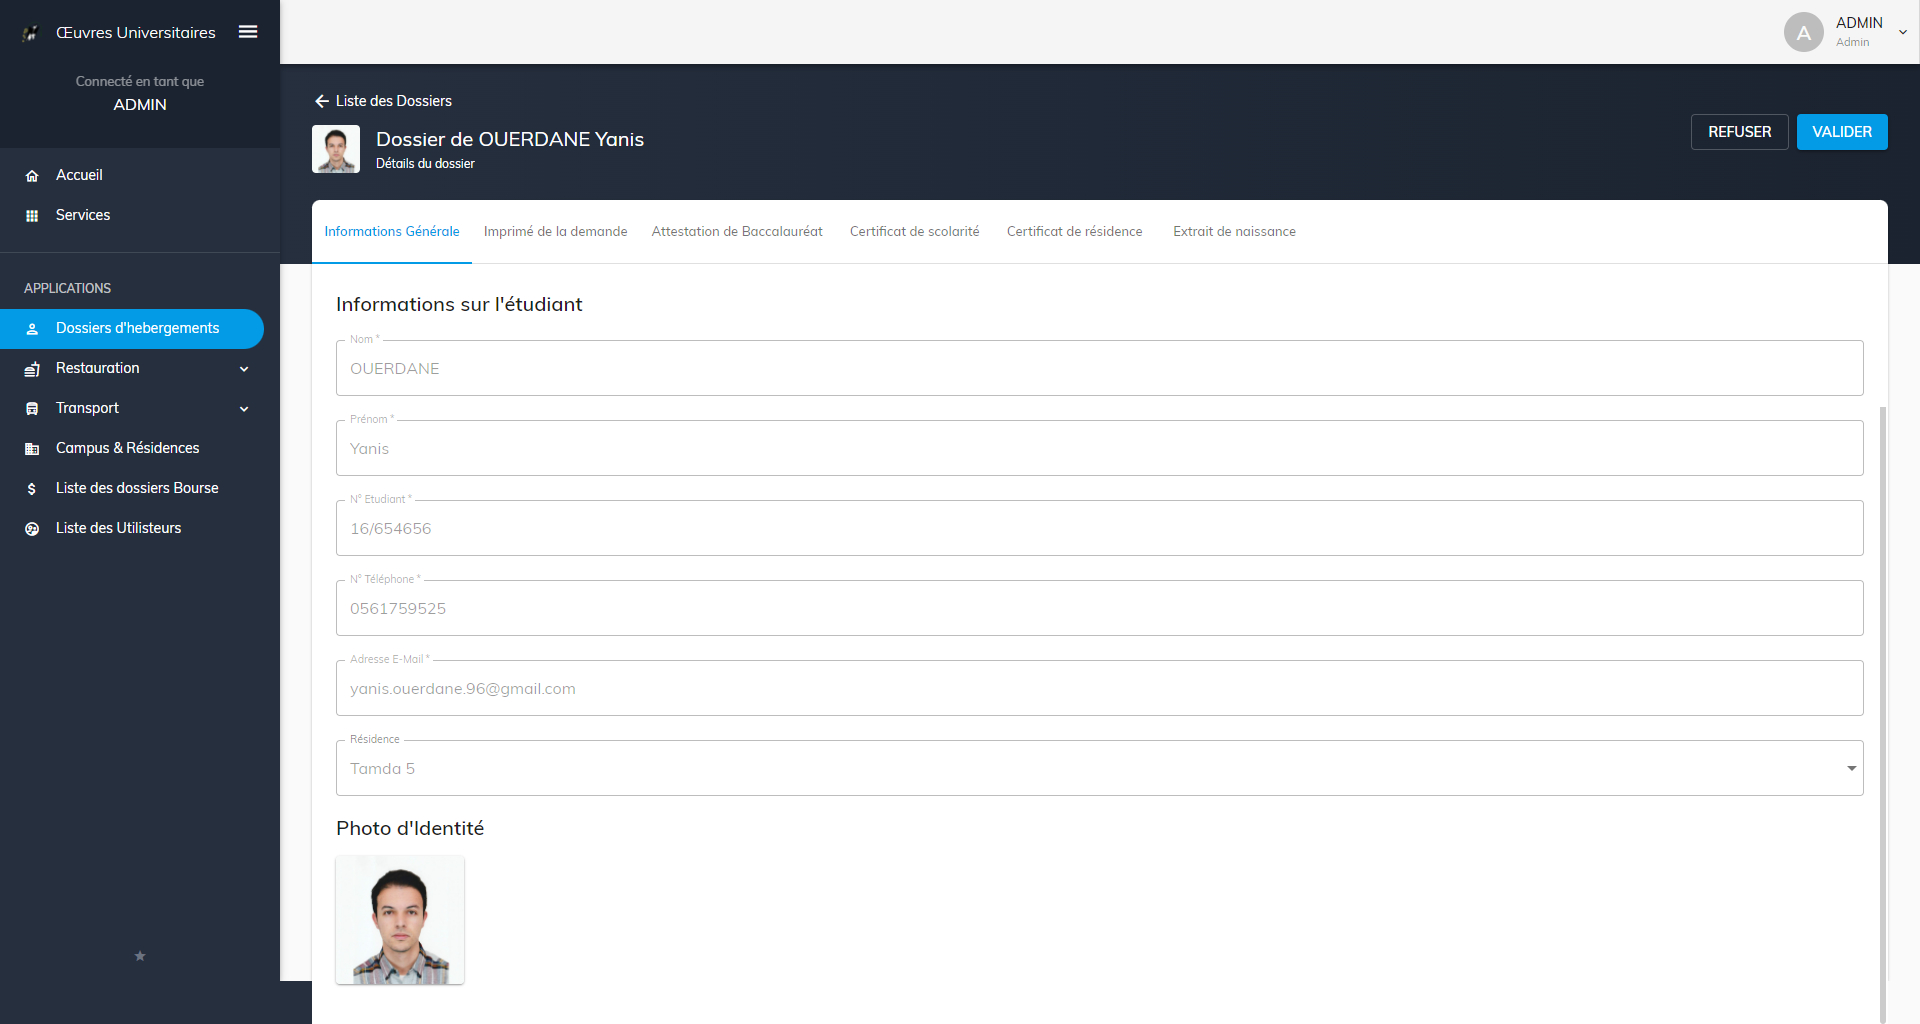
\includegraphics[scale=0.21]{PFE Screens/Admin/Hebergement/Detail.jpg}
        \caption{Interface utilisateur détail d'un dossier d'hebergements}
    \end{figure}

    \subsection{Interface utilisateur 'Liste des Réstaurants'}
    \begin{figure}[H]
        \centering
        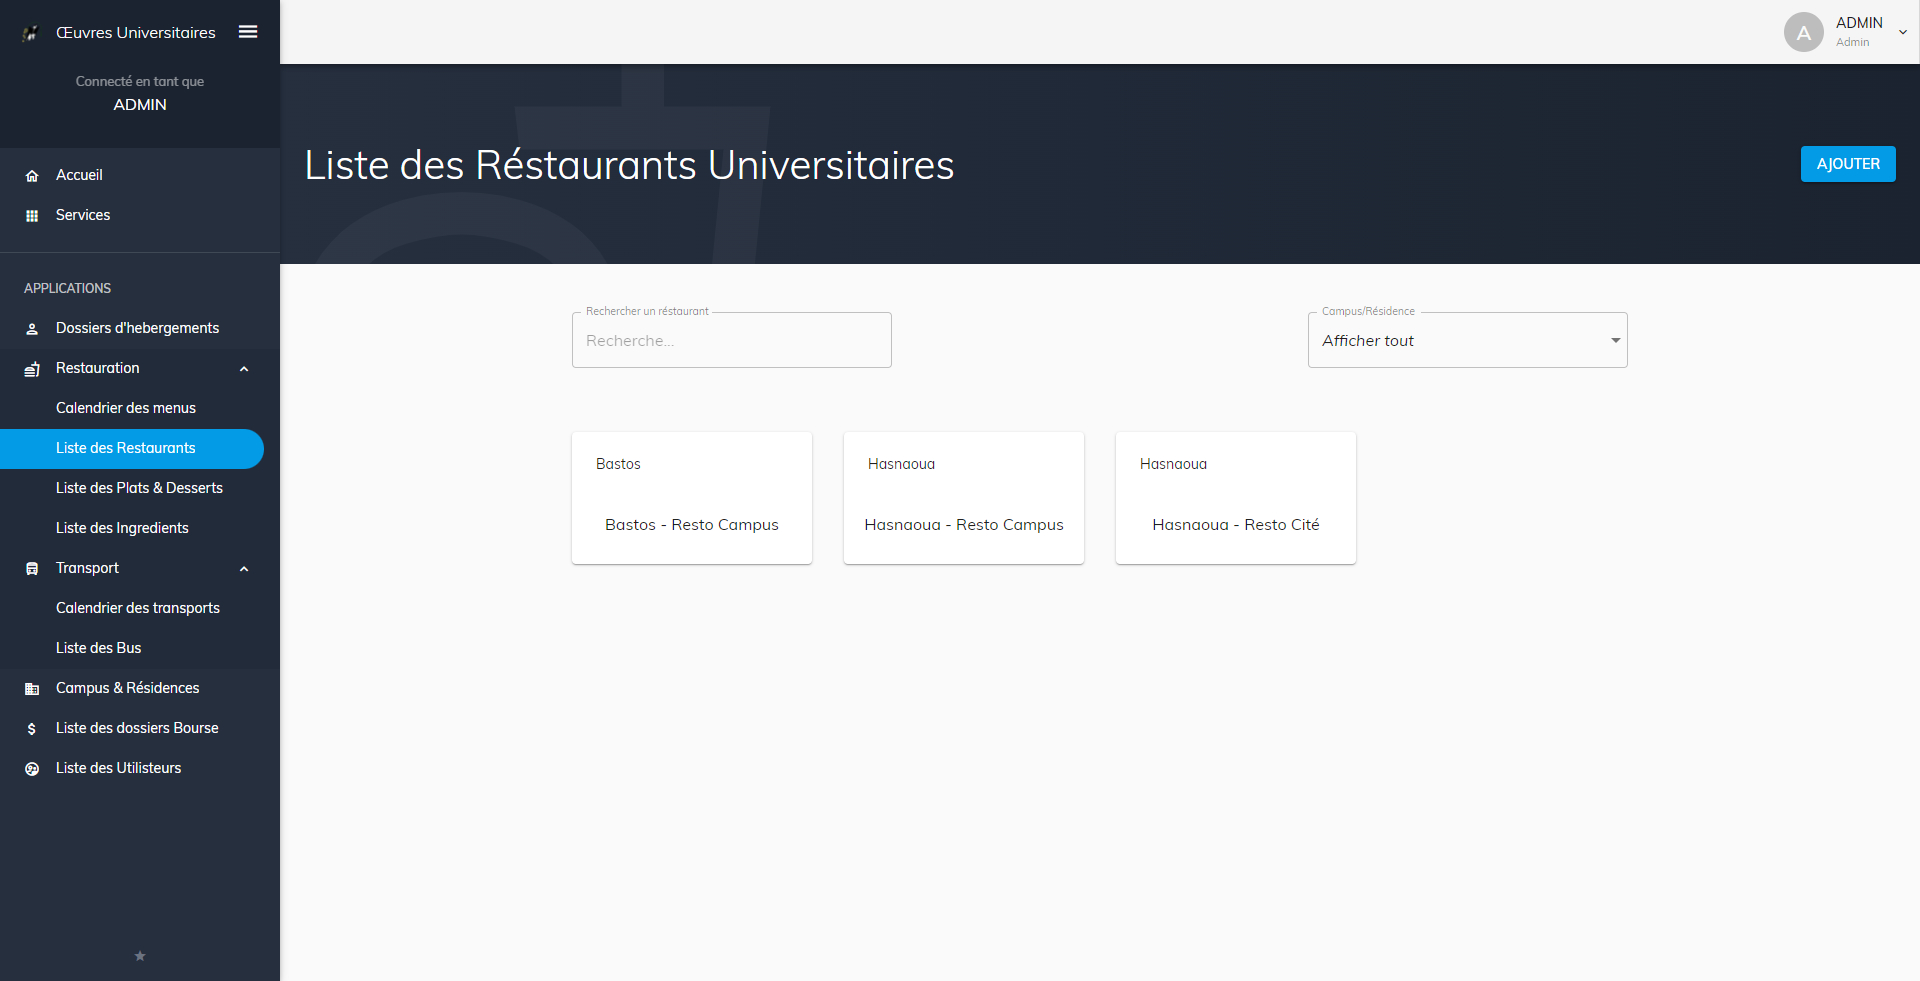
\includegraphics[scale=0.21]{PFE Screens/Admin/Restauration/Restos/Restos.jpg}
        \caption{Interface utilisateur 'Liste des Réstaurants'}
    \end{figure}

    \subsection{Interface utilisateur 'Modifier un réstaurant'}
    \begin{figure}[H]
        \centering
        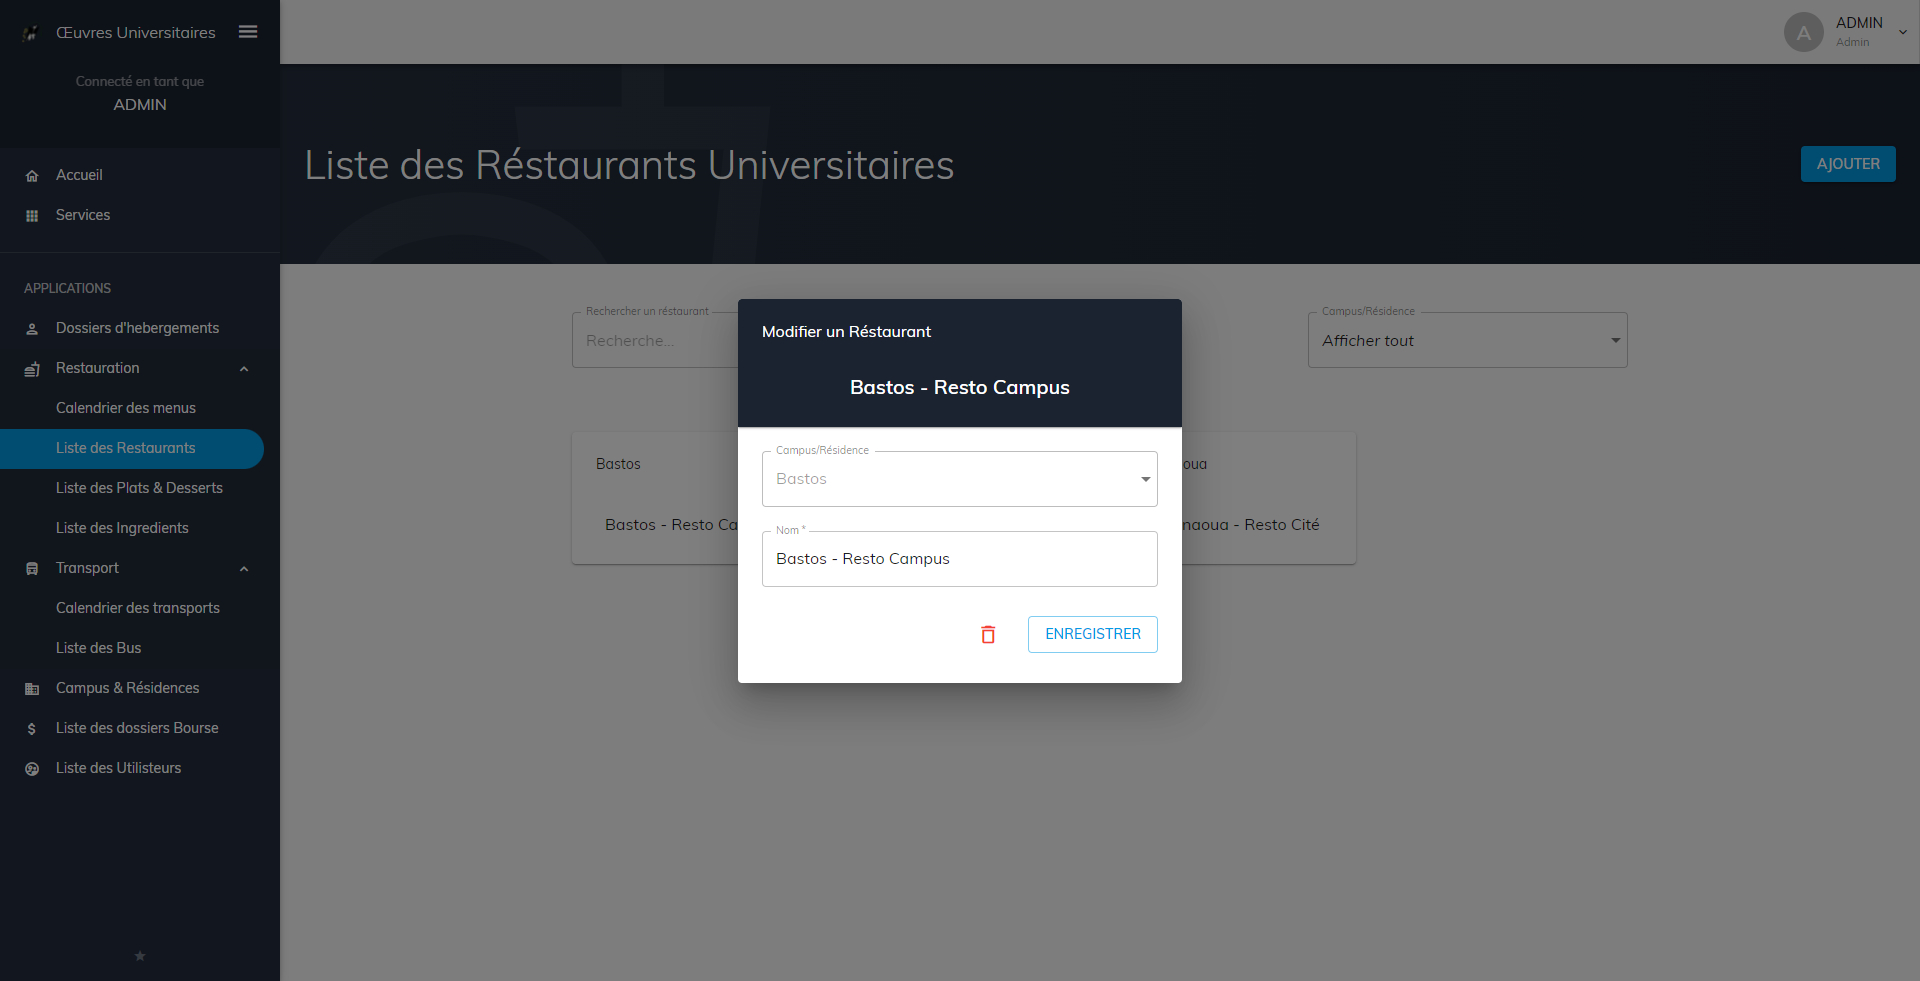
\includegraphics[scale=0.21]{PFE Screens/Admin/Restauration/Restos/Modif - Resto.jpg}
        \caption{Interface utilisateur 'Modifier un réstaurant'}
    \end{figure}

    \subsection{Interface utilisateur 'Liste des Ingredients'}
    \begin{figure}[H]
        \centering
        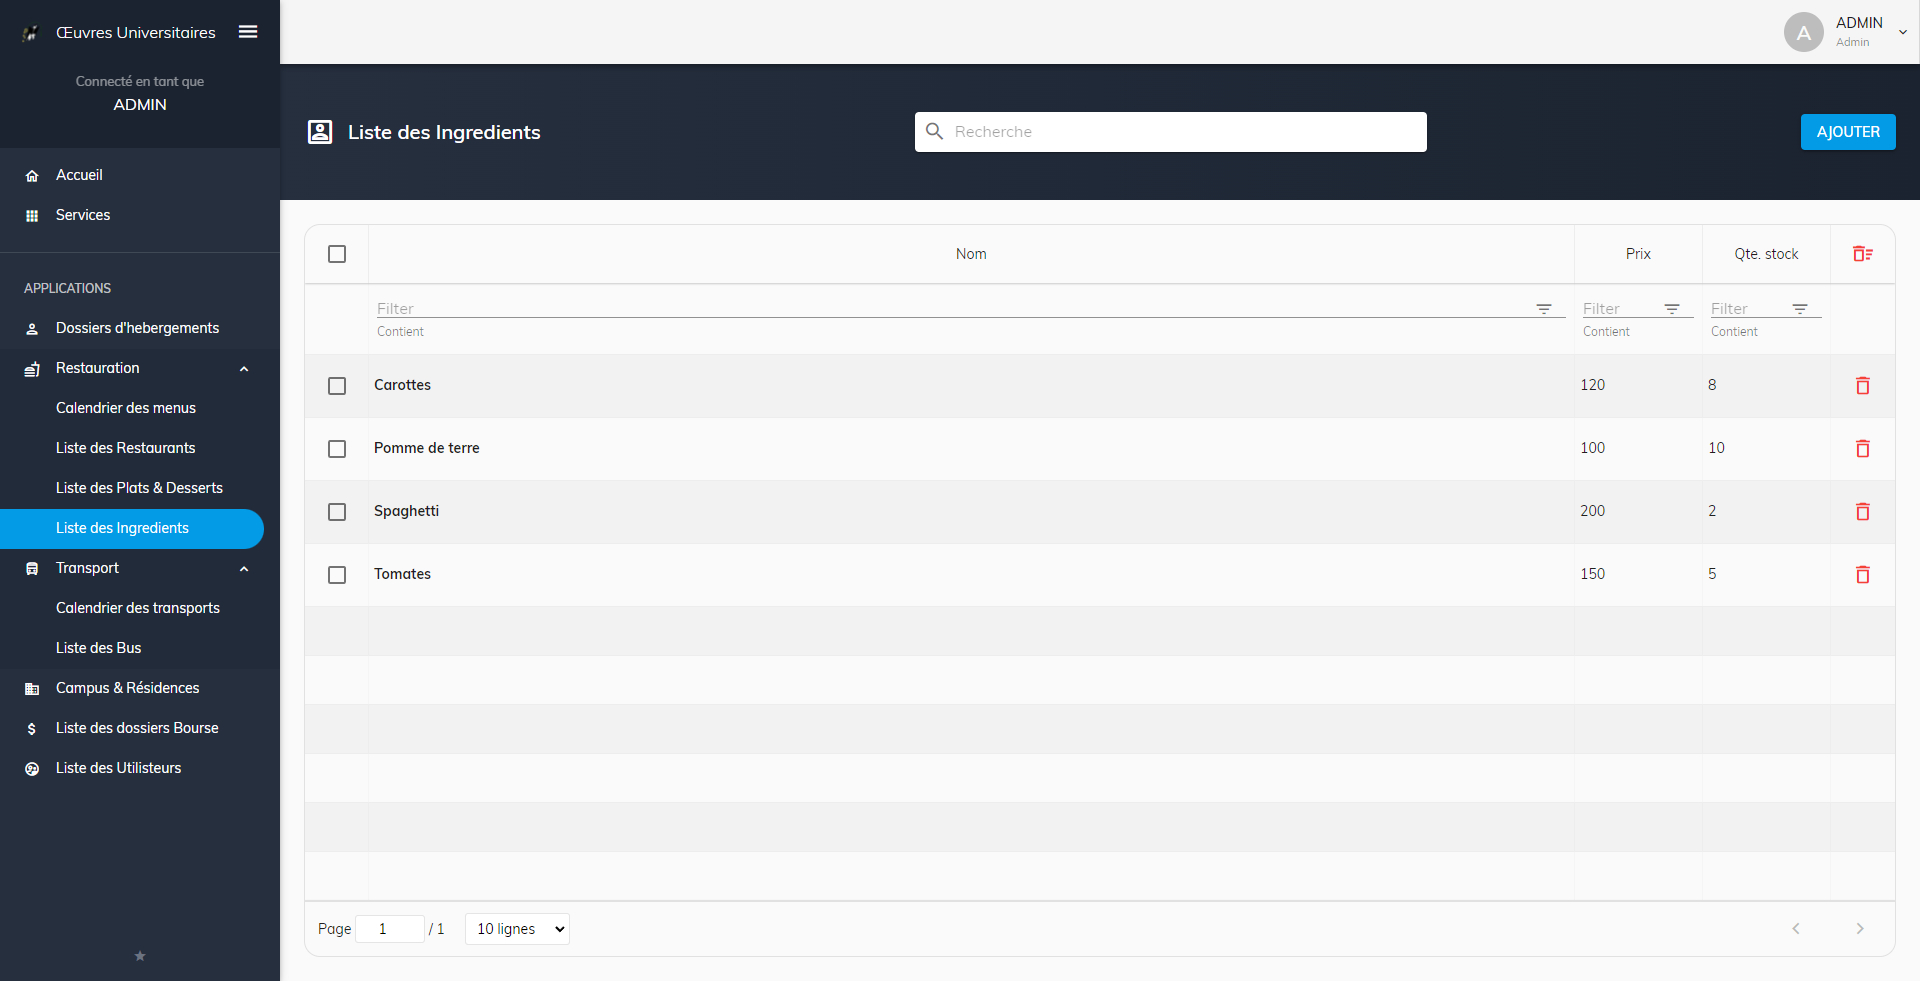
\includegraphics[scale=0.21]{PFE Screens/Admin/Restauration/Ingredients/liste.jpg}
        \caption{Interface utilisateur 'Liste des Ingredients'}
    \end{figure}
    
    \subsection{Interface utilisateur - Détails des menus du mois}
    \begin{figure}[H]
        \centering
        \includegraphics[scale=0.21]{PFE Screens/Admin/Restauration/Calendrier/Détails du moi.jpg}
        \caption{Interface utilisateur - Détails des menus du mois}
    \end{figure}

\section{Conclusion}
Dans ce chapitre nous avons montré l'environnement de travail, les outils utiliser pour créer notre application ainsi que les techniques et les bibliothèques qui nous ont aider dans ce processus.\\

Par la suite, nous avons présenté quelles ques interfaces du rendu final de notre application.\\

Tout en respectant le concept développé lors de l'analyse, nous avons pu réaliser les objectifs fixés.\\

	\part*{Conclusion Générale}
	\addcontentsline{toc}{part}{Conclusion Générale}
		% \renewcommand{\thechapter}{}
\renewcommand{\chaptername}{}
\chaptermark{Conclusion}

L'objectif de notre projet etait de concevoir une plateforme uniforme pour les directions des œuvres universitaires qui permettrait d'un coté a cette diréction un suivi en temps réel des ressources a leurs dispositions et une performance et des économies accrus grâce a un meilleur vue d'ensembles des mouvement de ces ressources, d'un autre coté aux étudiants de pouvoir accéder a plusieurs bout d'informations pertinante toujours au même et unique endroit.\\

Tout au long de ce mémoire nous avons présenté les différentes phases de réalisation de notre projet. Nous avons commencer par définir le progiciel de gestion interne aussi connu en tant que \acs{ERP}, nous avons parcouru son historique, et vue les avantages et les inconvenients de ce derniers. Ensuite, nous avons décrit les besoins des futurs utilisateurs en utilisant UML. Ceci a conduit à une analyse plus approfondie puis à la conception des fonctions applicatives que nous avons mises en œuvre dans le processus de production.\\

Cette dernière est basée sur des techniques fiables, puissantes et évolutives.Le front-end est géré par React qui est une bibliothèque Javascript très puissante. le back-end est construit a l'aide d'ExpressJS qui est une bibliothèque Javascript lui aussi qui est très versatile et très robuste. La base de données a été créée avec PostgreSQL qui est un gestionnaire de base de données qui utilise \acs{SQL} mais qui le complémente de manière a favorisé l'extensibilité et la conformité. Tout ceci viens s'emboiter de façons à ce que les éventuelles fonctionnalités qui viendront s'ajouter à celles déjà implémenté, tel que la gestion des ingrédients, la gestion des restaurants, la gestion des calen\acs{DRI} ers des menus et des transports, la gestion des dossiers d'hébergements et des dossiers bourse et bien d'autres, peuvent être ajoutées avec une grande simplicité.\\

Malgré les inconvénients et les limites imposées par certaines contraintes, qui ont créé plusieurs obstacles a l'amélioration de l'application. Réaliser une interface simple, intuitive et ergonomique et des fonctionnalités pratiques reste complexes en vue du besoin nécessaire d'un feedback régulier et directe de la part des futurs utilisateurs de cette application.\\

Cependant ce projet n'est qu'à son début et à beaucoup de potentiel d'amélioration avec l'intégration d'autres modules pour couvrir l'ensemble des besoins de la direction des œuvres universitaires. Ainsi que l'ajout et la modification de quelles ques fonctionnalités telles qu'un tableau de bord pour voir toutes les données pertinente dans une seule interface et la possibilité de changer de langues.\\

Commencer un projet à partir de zéro était une opportunité que vous devaient saisir. Ce projet nous a permis d'évoluer, d'approfondir et d'acquérir de nouvelles connaissances. Nous avons découvert et maitriser plusieurs outils, technologies et framework. Nous sommes donc fières de notre travail et nous sommes sur de pouvoir relever notre prochain défi.\\


	\leftskip=0cm
	\renewcommand{\bibname}{Référence bibliographique et webographique}
	\bibliographystyle{ieeetr}
	\bibliography{ERP/erp,DOU/dou,ACR/acr}
	
\end{document}
